\documentclass[11pt]{article}
\usepackage[T1]{fontenc}
\usepackage{lmodern}
\usepackage[margin=1in]{geometry}
\usepackage{amsmath,amssymb,amsthm,mathtools,mathrsfs}
\usepackage{microtype}
\usepackage{enumitem}
\usepackage{booktabs}
\usepackage{tikz}
\usetikzlibrary{arrows.meta,positioning}
\usepackage{xurl}
\usepackage[colorlinks=true,linkcolor=blue!45!black,citecolor=blue!45!black,urlcolor=blue!45!black]{hyperref}
\newtheorem{theorem}{Theorem}[section]
\newtheorem{proposition}[theorem]{Proposition}
\newtheorem{lemma}[theorem]{Lemma}
\newtheorem{corollary}[theorem]{Corollary}
\theoremstyle{definition}
\newtheorem{definition}[theorem]{Definition}
\theoremstyle{remark}
\newtheorem{remark}[theorem]{Remark}
\newtheorem{example}[theorem]{Example}
\newcommand{\OO}{\mathcal O}
\newcommand{\EE}{E}
\newcommand{\QQ}{\mathbb Q}
\newcommand{\ZZ}{\mathbb Z}
\newcommand{\FF}{\mathbb F}
\newcommand{\kk}{k}
\newcommand{\eps}{\varepsilon}
\newcommand{\Qbar}{\overline{\mathbb Q}}
\newcommand{\Fbar}{\overline{\mathbb F}}
\newcommand{\GQ}{G_{\mathbb Q}}
\newcommand{\GQtwo}{G_{\mathbb Q_2}}
\DeclareMathOperator{\GL}{GL}
\DeclareMathOperator{\SL}{SL}
\DeclareMathOperator{\PGL}{PGL}
\DeclareMathOperator{\Gal}{Gal}
\DeclareMathOperator{\Spec}{Spec}
\DeclareMathOperator{\Supp}{Supp}
\DeclareMathOperator{\Frac}{Frac}
\DeclareMathOperator{\tr}{tr}
\DeclareMathOperator{\ad}{ad}
\DeclareMathOperator{\Hom}{Hom}
\DeclareMathOperator{\End}{End}
\DeclareMathOperator{\Ind}{Ind}
\DeclareMathOperator{\cInd}{c-Ind}
\DeclareMathOperator{\WD}{WD}
\DeclareMathOperator{\HT}{HT}
\DeclareMathOperator{\Fil}{Fil}
\DeclareMathOperator{\Ann}{Ann}
\DeclareMathOperator{\rank}{rank}
\DeclareMathOperator{\im}{im}
\DeclareMathOperator{\coker}{coker}
\DeclareMathOperator{\codim}{codim}
\setlist[enumerate]{itemsep=3pt,topsep=5pt}
\setlist[itemize]{itemsep=3pt,topsep=5pt}
\setcounter{tocdepth}{2}
\title{Fontaine--Mazur modularity at the prime 2}
\author{OpenAI}
\date{October 6, 2026}

\hypersetup{pdftitle={Fontaine--Mazur modularity at the prime 2},pdfauthor={OpenAI},pdfsubject={Odd regular two-dimensional Fontaine--Mazur modularity at 2}}

\begin{document}
\maketitle
\begin{abstract}
We prove that every continuous, irreducible, odd two-dimensional
\(2\)-adic representation of \(G_{\mathbb Q}\), unramified outside
finitely many primes and de Rham at \(2\) with distinct Hodge--Tate
weights, is modular up to Tate twist. This resolves the odd, regular
two-dimensional Fontaine--Mazur conjecture over \(\mathbb Q\) at \(2\),
including all residual representations.
\end{abstract}

\section{Introduction}\label{sec:introduction}

The Fontaine--Mazur conjecture predicts that irreducible \(p\)-adic
Galois representations satisfying suitable finiteness and local
conditions arise from algebraic geometry \cite{FM1995}. Modular forms supply
a central class of examples through Deligne's cohomological construction
\cite[Sections~3.9--3.12 and~5.2--5.5]{Deligne1971}. Over
\(\mathbb Q\), its odd two-dimensional form has a more precise
modularity formulation. A continuous representation
\[
 r:G_{\mathbb Q}\longrightarrow\GL_2(\overline{\mathbb Q}_p)
\]
is \emph{odd} if \(\det r(c)=-1\) for a complex conjugation \(c\).
It is \emph{regular de Rham} at \(p\) if its restriction to
\(G_{\mathbb Q_p}\) is de Rham and has two distinct Hodge--Tate
weights. The conjecture asserts that an irreducible such
representation, unramified outside finitely many primes, comes
from a classical cuspidal eigenform, allowing a Tate twist.

\begin{theorem}\label{thm:main}
Let
\[
 r:G_{\mathbb Q}\longrightarrow\GL_2(\overline{\mathbb Q}_2)
\]
be continuous and irreducible. Suppose that \(r\) is odd, is
unramified outside finitely many primes, and is de Rham at \(2\)
with distinct Hodge--Tate weights. Then \(r\) is isomorphic to
a Tate twist of the \(2\)-adic Galois representation associated
with a classical cuspidal eigenform.
\end{theorem}

Thus Theorem~\ref{thm:main} resolves the odd, regular two-dimensional
Fontaine--Mazur conjecture over \(\mathbb Q\) at \(2\). Its scope includes
every semisimple residual representation, including scalar and reducible
ones. Together with the odd-prime results discussed below, it gives the
stated modularity conclusion at every prime. The geometric realization
of modular representations also gives the geometric-origin conclusion
in this odd, regular setting.

Theorem~\ref{thm:main}, in particular its absence of a residual-image
hypothesis, supplies the weight-two modularity input in the height argument
of \emph{Hilbert's tenth problem over the rational numbers}
\cite[Section~4]{OpenAIH10Q2026}, whose undecidability proof also uses
substantial additional arithmetic and logical constructions.

\subsection{Background and the dyadic problem}

The deformation-theoretic approach to modularity lifting developed
by Wiles and Taylor--Wiles compares Galois deformation rings with
Hecke algebras \cite{Wiles1995,TaylorWiles1995}. Serre's conjecture
concerns the residual starting point \cite{Serre1987}; its proof by
Khare--Wintenberger and Kisin supplies modularity for odd absolutely
irreducible residual representations, including characteristic two
\cite{KhareWintenberger2009,KhareWintenberger2009II,Kisin2009}.
The existence of a residual modular form still leaves the problem
of proving modularity for a specified characteristic-zero lift.
For a reducible residual representation, even the modular seed
must be obtained by a different construction.

Skinner and Wiles developed ordinary families and pro-modularity
arguments for residually reducible representations and then for
nearly ordinary deformations of irreducible residual representations
\cite{SkinnerWiles1999,SkinnerWiles2001}. Allen adapted this family
method to nearly ordinary dyadic representations with solvable
absolutely irreducible residual image \cite{Allen2014}.
Kisin brought local deformation geometry and the $p$-adic
Langlands correspondence into the regular Fontaine--Mazur problem
\cite{Kisin2009FM}. Emerton's local--global compatibility work
separated occurrence in completed cohomology from the production
of classical vectors \cite{Emerton2011}. These developments
explain why both stages of the proof below are needed, and why
ordinary auxiliary families can be useful without ordinarity
being imposed on the final target.

At odd primes, Pan's work treats the residually reducible case and,
together with preceding modularity lifting theorems, establishes the
regular conjecture apart from one local residual configuration at~$3$
\cite[Theorems~1.0.2 and~1.0.4]{Pan2022}. Zhang removes that
configuration, obtaining the stated odd, regular theorem for every
odd prime \cite[Theorem~1.0.2]{Zhang2025}. At~$2$, Tung removes
the remaining local restriction in a modularity lifting theorem whose
global residual image is nonsolvable
\cite[Theorem~A]{Tung2021Dyadic}. Thus local scalar residual
behavior and a globally scalar residual representation must be
distinguished: a local theorem covering the former does not by
itself settle the latter.

The proof has a useful precedent in the passage from unrestricted
pro-modularity to classicality developed by Pan, and in Zhang's
potential pro-modularity argument \cite{Pan2022,Zhang2025}.
The present dyadic problem requires integral control of the local
actions and of deformation families even when their residual
representation is scalar. We first construct potential occurrence
in completed definite forms, then extract classical vectors, and
finally descend. The distinction between occurrence and classicality
also appears in Pan's theorem for representations in the completed
cohomology of modular curves: that theorem assumes occurrence as
a hypothesis \cite[Theorem~7.1.2]{Pan2026Classicality}.

Thorne's theorem supplies an essential set of classical points:
ordinary, potentially crystalline representations of weights
$\{0,1\}$ are modular at every prime, without a residual
irreducibility hypothesis \cite[Theorem~D]{Thorne2026}.
After a global normalization and passage to the dual, our family
construction makes this theorem applicable at a dense
set of points, and the subsequent specialization argument recovers
the original target's arbitrary weight gap. Prescribing global
lifts with chosen local components, as in Emerton--Gee--Pan--Zhu
\cite[Theorem~1.1.1]{EGPZ2026}, is a different conclusion;
their dyadic theorem also retains a nonsolvable residual-image
hypothesis.

The local input is the \(p\)-adic Langlands correspondence of
Colmez~\cite{Colmez2010}, in the all-prime form of Colmez, Dospinescu
and Pa\v{s}k\=unas~\cite{CDP2014}. Pa\v{s}k\=unas and Tung's block
finiteness theorem~\cite{PaskunasTung2021} supplies an integral local
pseudodeformation action even in scalar residual blocks. This resolves
a local representation-theoretic obstacle, but leaves a global one:
a trace does not record a residual extension class, and globally
reducible families can be too large for a direct connectedness argument.
We work with actual representations and temporarily record local
invariant lines to obtain the necessary dimension loss. These auxiliary
marks are used in connectedness; the propagation theorem imposes no
ordinary condition at the dyadic places.

\subsection{From occurrence to classicality and descent}

A \emph{pro-modular locus} is a closed trace locus in a Galois
pseudodeformation spectrum defined by a completed Hecke algebra of
definite quaternionic forms. No local condition is imposed at~\(2\).
Its characteristic-zero points give Hecke eigensystems in completed
forms. The central problem is to pass from this occurrence statement
to a classical cuspidal form with the prescribed Galois representation.
We do so in three stages, summarized in Figure~\ref{fig:proof-route}.

\paragraph{Potential occurrence for a whole family.}
The first stage places the target and the deformation families needed
later in one pro-modular trace locus over a common solvable totally
real extension \(F\), completely split at~\(2\). Two constructions
work together. Localized propagation starts at a characteristic-two
curve whose generic representation remains absolutely irreducible
under finite restriction. If the curve is pro-modular and has finite
local images at the allowed non-dyadic primes, patching gives
potential pro-modularity of every irreducible deformation locus
containing it (Theorem~\ref{thm:localized-propagation}). The local
deformation problem at~\(2\) is unrestricted.

To produce the curves to which this result applies, we construct
abelian \(2\)-extensions \(\mathbb Q\subset A\subset F\), keeping the
number of allowed ramified primes under control while their degrees
grow. In the scalar and reducible cases we mark a small proportion of
the dyadic places. Recording an invariant line at those places retains
information that traces alone would lose. We select the open part of
the residual fiber on which the marked lines are transverse to every
globally invariant line. A Selmer calculation makes the globally
reducible locus too small to disconnect these charts. A modular seed
and a curve cut from a component containing the target enter the same
connected residual fiber. Applying propagation along it yields
Theorem~\ref{thm:potential-promodularity}. The conclusion concerns the
whole closed trace image of the prescribed family at one common tame
level; it does not require that this family itself have the dimension
of the larger component used to find the curve.

\paragraph{Classical vectors at the target.}
When the local representation at~\(2\) is irreducible, the local
Langlands correspondence supplies locally algebraic vectors. For a
reducible local target, we choose an invariant line with the larger
cyclotomic exponent and retain its character as a parameter. The
resulting family records trace and character jointly and is finite
over a one-dimensional weight space. Its continuous members are not
all de Rham; the useful points are a dense set of specially chosen
weights. After a global twist the corresponding representations have
cyclotomic exponents \(\{1,0\}\), or Hodge--Tate weights
\(\{-1,0\}\). Their \emph{duals} have Hodge--Tate weights
\(\{0,1\}\) and satisfy the ordinary potentially crystalline
hypotheses of Thorne's theorem.

Those classical points determine the order of the two characters in
the ordinary induction. A finite closed joint support transports this
order to the target. A quotient, lattice and Tate-module construction
then supplies a genuine eigenvector in the target eigenspace. Finally,
a direct polynomial-orbit argument turns its character and exponent
inequality into a nonzero locally algebraic vector. This last step
avoids assuming that algebraic vectors commute with specialization.

\paragraph{Descent of a classical packet.}
The vector gives a regular cuspidal automorphic representation over
\(F\). We descend along prime-degree cyclic steps in a solvable tower.
At each step, a finite-character discrepancy between the descended
Galois representation and the target is removed by a Hecke-character
twist. Descent is applied only after classicality has been established;
no descent statement for pro-modular loci is needed.

\begin{figure}[tp]
\centering
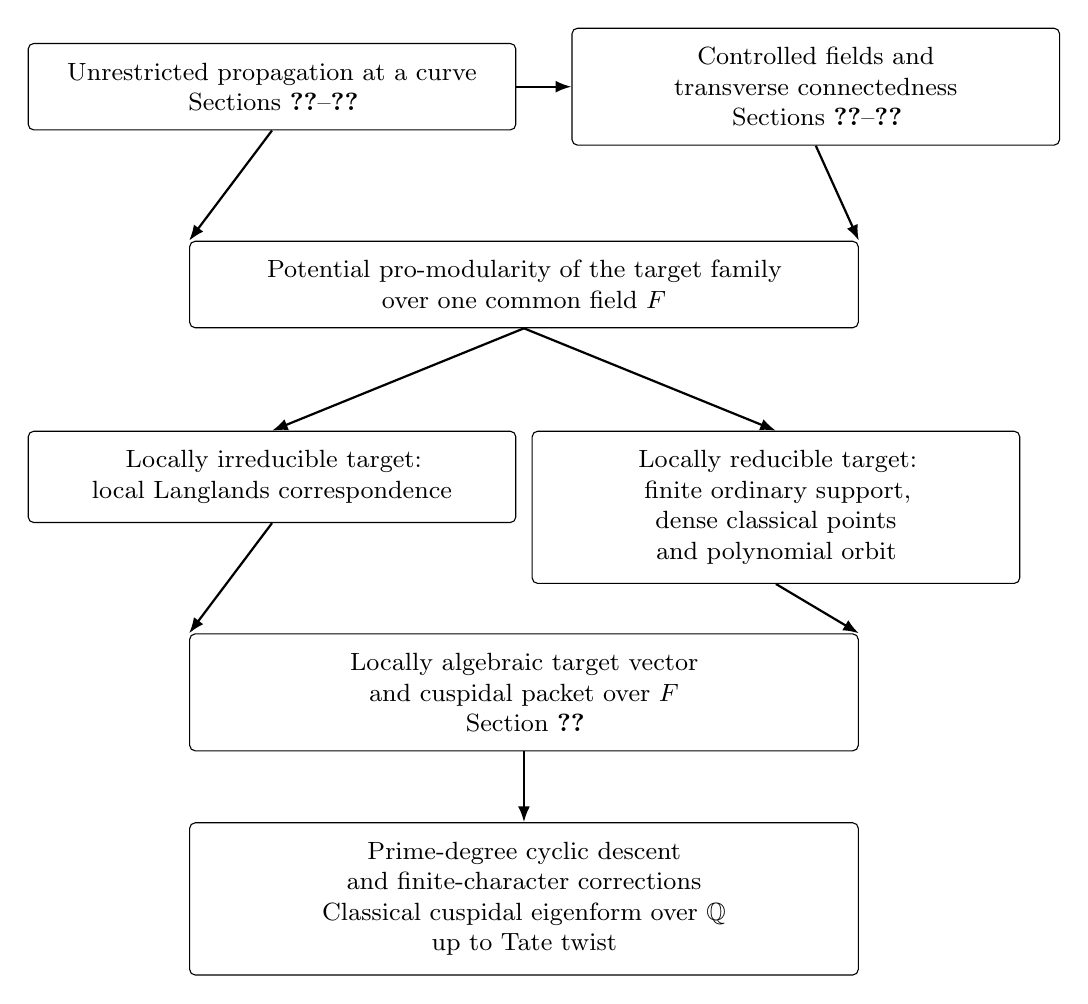
\begin{tikzpicture}[
 box/.style={draw,rounded corners=2pt,align=center,font=\small,
 text width=5.7cm,inner sep=7pt},
 arr/.style={-{Latex[length=2mm]},thick},node distance=9mm]
\node[box] (prop) {Unrestricted propagation at a curve\\
Sections~\ref{sec:deformation}--\ref{sec:propagation}};
\node[box,right=7mm of prop] (conn) {Controlled fields and transverse connectedness\\
Sections~\ref{sec:fields}--\ref{sec:connectedness}};
\draw[arr] (prop.east) -- (conn.west);
\node[box,below=14mm of prop,xshift=3.2cm,text width=8cm] (occ)
{Potential pro-modularity of the target family\\over one common field \(F\)};
\draw[arr] (prop.south) -- (occ.north west);
\draw[arr] (conn.south) -- (occ.north east);
\node[box,below=13mm of occ,xshift=-3.2cm] (irr)
{Locally irreducible target:\\local Langlands correspondence};
\node[box,below=13mm of occ,xshift=3.2cm] (red)
{Locally reducible target:\\finite ordinary support,\\dense classical points\\and polynomial orbit};
\draw[arr] (occ.south) -- (irr.north);
\draw[arr] (occ.south) -- (red.north);
\node[box,below=14mm of irr,xshift=3.2cm,text width=8cm] (vec)
{Locally algebraic target vector\\and cuspidal packet over \(F\)\\
Section~\ref{sec:classicality}};
\draw[arr] (irr.south) -- (vec.north west);
\draw[arr] (red.south) -- (vec.north east);
\node[box,below=of vec,text width=8cm] (end)
{Prime-degree cyclic descent and finite-character corrections\\
Classical cuspidal eigenform over \(\mathbb Q\)\\up to Tate twist};
\draw[arr] (vec) -- (end);
\end{tikzpicture}
\caption{The proof route. The connectedness construction uses the
propagation theorem; the two upper boxes are cooperating inputs to
occurrence. The target enters through that construction. The common
field \(F\) is solvable, totally real, of even degree and completely
split at~\(2\). The ordinary family is used in the reducible local
branch. Both branches produce a classical packet before descent.}
\label{fig:proof-route}
\end{figure}

\subsection{The constructions used in the proof}

Several established methods must be kept compatible at the
characteristic-two curve. B\"ockle--Iyengar--Pa\v{s}k\=unas develop
local deformation theory with Laurent-series residue fields and
coefficient orders, including the auxiliary-variable comparison of
completions \cite[Section~3.5]{BIP}. We use this framework
with an extra coefficient variable and global representation and
incidence spaces. Lemma~\ref{lem:curve-completion} proves the resulting
identification of continuous deformation and obstruction problems,
including the topology on the residue field and the dimension change.

The propagation construction follows the auxiliary-level method of
Taylor--Wiles, Kisin's formulation relative to local deformation rings,
and the characteristic-two determinant-twist argument of
Khare--Wintenberger
\cite{TaylorWiles1995,Kisin2009FiniteFlat,KhareWintenberger2009II}.
Pan's localization at one-dimensional primes is the direct global
precedent \cite{Pan2022}; Zhang's potential formulation is used in
the same overall progression \cite{Zhang2025}. At the Laurent-series
residue field we patch finite jets, meaning quotients by fixed powers
of the local maximal ideal. The exactness argument works with
filtrations whose successive quotients are fixed old-level modules.
A uniform Artin--Rees bound preserves their actual old deformation
actions. Determinant twists and explicit quadratic sign intertwiners
then give support on every local component. All of these action
comparisons are retained integrally.

The marked-line construction serves a different purpose. Its local
factors are integral even over the characteristic-two real-place
base, and transversality gives a strict Selmer loss at every mark.
The number of marks grows more slowly than the total degree, so this
loss is compatible with the global dimension estimates. The argument
uses the unrestricted propagation theorem after entering a transverse
chart; it does not replace that theorem by ordinary patching.

\paragraph{Organization.}
Section~\ref{sec:preliminaries} fixes conventions and removes the
virtually solvable case. Section~\ref{sec:deformation} constructs the
representation spaces, their curve completions and the local models.
Section~\ref{sec:completed} compares the actual Galois and local
block actions on completed forms and proves the Hecke-dimension bound.
Section~\ref{sec:propagation} proves localized propagation.
Section~\ref{sec:fields} supplies the field and Selmer estimates, and
Section~\ref{sec:connectedness} combines them with a modular seed to
obtain potential pro-modularity. Section~\ref{sec:classicality}
constructs classical vectors and carries out solvable descent.

\clearpage
\begingroup
\small
\tableofcontents
\endgroup
\clearpage
\section{Conventions and initial reductions}\label{sec:preliminaries}

We fix the coefficient and automorphic conventions before
introducing deformation spaces. We then remove the virtually
solvable case and specify the trace loci used throughout the
proof. Table~\ref{tab:conventions} collects the normalizations that
link deformation theory, completed forms and classicality.

\begin{table}[htbp]
\centering\small
\renewcommand{\arraystretch}{1.2}
\begin{tabular}{@{}p{0.23\textwidth}p{0.70\textwidth}@{}}
\toprule
Object & Convention \\
\midrule
Frobenius & Geometric by default; local reciprocity sends a uniformizer
to geometric Frobenius. The tame relation with exponent \(q_v\)
uses arithmetic Frobenius explicitly. \\
Weights & \(\eps=x|x|\), cyclotomic exponent \(1\),
\(\HT(\eps)=\{-1\}\), and \(|2|=2^{-1}\). \\
Determinants and blocks & \(\chi=\det r\), completed-form central
character \(\psi=\chi\eps\), local block parameter \(r\otimes\eps\)
with determinant \(\chi\eps^2\). \\
Ordinary target & At a locally reducible de Rham target choose the line character
\(\eta_1\) with exponent \(a>b\), where
\(\eta_2=\chi/\eta_1\) has exponent \(b\). The favorable upper-Borel,
unnormalized inducing pair is \((\eta_2\eps,\eta_1)\). \\
Algebraic factor & \(\operatorname{Sym}^{a-b-1}\det^{b+1}\).
The continuous family retaining \(\eta_1\) need not be de Rham. \\
Curve coefficients & \(K=k((t))\) has its Laurent topology;
\(\mathcal L=\widehat{\OO[[z]]_{(\varpi)}}\), with \(z\mapsto t\).
The auxiliary ultrapower in Section~\ref{sec:propagation} is specified
separately. \\
Dual actions & Group duals use the indicated contragredient action.
On scalar eigenspaces the commuting Hecke, torus and \(U\) operators
are transposed without inversion, as in Section~\ref{sec:classicality}. \\
Support & Images in pseudodeformation spectra are closed images;
pro-modular support containments are set-theoretic. \\
\bottomrule
\end{tabular}
\caption{Conventions used at the interfaces of the proof. The
character orientation in the table concerns the chosen target and
the normalized dense points, not every member of the family.}
\label{tab:conventions}
\end{table}

\subsection{Coefficients and cyclotomic exponents}

Write \(\OO\) for the ring of integers in a sufficiently large
finite extension \(E/\mathbb Q_2\), \(\varpi\) for a uniformizer,
and \(k\) for its residue field. Finite coefficient extensions
are allowed. A lattice means a finite free \(\OO\)-module of
full rank. The cyclotomic character is denoted by \(\eps\).
We count weights as \emph{cyclotomic exponents}, so that
\(\eps\) has exponent \(1\). In the Hodge--Tate convention
\(\HT(\eps)=\{-1\}\), exponents are the negatives of
Hodge--Tate weights.

We use geometric Frobenius and local reciprocity sending a
uniformizer to geometric Frobenius. Thus, as a character of
\(\mathbb Q_2^\times\),
\[
 \eps=x|x|,\qquad x(a)=a.
\]
The determinant of a Galois representation is denoted by
\(\chi\). For a representation in Theorem~\ref{thm:main},
de Rham class field theory gives
\[
 \chi=\chi_{\mathrm{fin}}\eps^w
\]
for a finite-order character \(\chi_{\mathrm{fin}}\) and an
integer \(w\). Indeed, Tate's local algebraicity theorem
\cite[Chapter~III, Section~1.2]{Serre1989Abelian} gives the integral
cyclotomic exponent at~\(2\). Removing this power leaves a character
locally constant at every finite place. Finite ramification and global
reciprocity make it a character of a finite ray class group, hence of
finite order.
In the convention for quaternionic forms
used below, the central character is
\[
 \psi=\chi\eps.
\]
The normalized local block parameter attached to a Galois
representation \(\rho\) is that of \(\rho\otimes\eps\).
These conventions agree with \cite[Sections~3.1--3.5]{Pan2022}.

For the statement of Theorem~\ref{thm:main}, one may use the arithmetic
normalization \(V_f\) of the representation of a primitive eigenform
of weight \(k\) and nebentype \(\psi_f\): at a good prime \(q\),
\[
 \tr V_f(\operatorname{Frob}^{\mathrm{ar}}_q)=a_q(f),\qquad
 \det V_f=\psi_f\eps^{k-1}.
\]
These trace and determinant formulas use the normalization of
\cite[Theorem~6.1]{DeligneSerre1974}; arithmetic Frobenius is fixed
there in Section~3.1. The cyclotomic exponents of \(V_f\) are
\(\{0,k-1\}\). Evaluating the same
representation at geometric Frobenius inverts its eigenvalues; it
does not change the representation into its dual. If a construction
instead produces \(V_f^\vee\), the wedge pairing gives
\[
 V_f^\vee\simeq V_f\otimes\psi_f^{-1}\eps^{1-k}
       \simeq V_g\otimes\eps^{1-k},
\]
where \(g\) is the primitive form associated with the finite-character
twist \(f\otimes\psi_f^{-1}\). Thus an expression
\(r\simeq V_f^\vee\eps^n\) becomes
\(r\simeq V_g\eps^{n+1-k}\). The up-to-Tate-twist conclusion of the
main theorem is unchanged by this conversion.

\begin{lemma}\label{lem:finite-coefficients}
A continuous finite-dimensional representation of a profinite
group on \(\overline{\mathbb Q}_2^n\) is defined over a finite
extension of \(\mathbb Q_2\) and admits a stable lattice there.
\end{lemma}
\begin{proof}
There are countably many finite subextensions of
\(\overline{\mathbb Q}_2/\mathbb Q_2\). For each one \(E\),
the set of group elements whose representation matrices
lie in \(\GL_n(E)\) is a closed subgroup. These subgroups
cover the profinite group. By Baire's theorem, one has
nonempty interior, hence is open. Enlarge \(E\) to contain
the finitely many matrix entries of coset representatives.
Then every matrix lies in that finite extension.

The image is compact. Its entries, and the entries of its
inverses, have bounded valuations. The \(\OO\)-submodule
generated by the orbit of \(\OO^n\) therefore lies between
two scalar multiples of \(\OO^n\). It is a stable lattice.
\end{proof}

We apply Lemma~\ref{lem:finite-coefficients} whenever a
characteristic-zero representation is first introduced.
Over a curve field, the analogous compact-image lattice
argument gives an integral realization over \(k'[[t]]\).

\subsection{The virtually solvable case}

For a representation over any field, after extending scalars
to an algebraic closure, call it \emph{virtually solvable}
if the identity component of the reduced Zariski closure of its image
is solvable. The closure here is taken over the algebraic closure,
so that the resulting algebraic group is smooth. This property is unchanged by restriction to
a finite-index subgroup.

\begin{lemma}\label{lem:solvable-reduction}
Theorem~\ref{thm:main} holds for virtually solvable
representations. A representation satisfying its hypotheses
and not virtually solvable remains absolutely irreducible
and not virtually solvable over every finite extension of
\(\mathbb Q\).
\end{lemma}
\begin{proof}
Let \(H\) be the algebraic monodromy group of an irreducible
two-dimensional representation over an algebraic closure.
Lie--Kolchin and the structure of connected solvable groups
\cite[Theorems~17.4 and~16.33]{MilneAlgebraicGroups} give the following
alternatives. If \(H^\circ\) is solvable and has a nontrivial unipotent
radical, the latter has a unique fixed line; normality
makes that line \(H\)-stable, contradicting irreducibility.
The remaining possibilities are that \(H^\circ\) is scalar,
or that its two distinct character lines are permuted by
\(H\).

In the scalar case the projective image is finite. After a
finite extension of the base field, the representation is
a scalar character on a two-dimensional space. Its two
Hodge--Tate weights are equal, which is excluded. In the
second case the action on the two lines gives a quadratic
extension \(L/\mathbb Q\) and
\[
 r\simeq\Ind_{G_L}^{G_{\mathbb Q}}\theta
\]
for a continuous character \(\theta\).
The character is de Rham and finitely ramified, hence is the
\(2\)-adic avatar of an algebraic Hecke character, by the
following rank-one consequence of Tate's theorem and the construction
in \cite[Chapter~III, Sections~1.2 and~2.3]{Serre1989Abelian}.
The integral algebraic exponents on open local units obey the global
unit relation. Principal ideals in a suitable ray subgroup therefore
receive the prescribed algebraic monomials. A positive power of each
of finitely many ray-class representatives is principal in that
subgroup, so its character value is algebraic. Adjoining these values
places all ideal-character values in one number field and constructs
the algebraic Hecke character. This argument does not assume that the
given character was initially rational over a number field.
If \(L\)
is real quadratic, its algebraic exponents at the two real
embeddings are equal by the unit theorem: a unit of infinite
order forces their difference to vanish in the algebraic
character relation. This again contradicts regularity.
For imaginary quadratic \(L\), the theta-series construction
gives the required cuspidal eigenform, with its algebraic
Tate normalization; equivalently, use quadratic automorphic
induction \cite[Proposition~12.1]{JacquetLanglands1970}.

Finally, restriction to finite index preserves \(H^\circ\).
If a restriction of a non-virtually-solvable representation
were reducible, its identity component would lie in a
Borel subgroup and be solvable. This is impossible.
\end{proof}

Henceforth the target \(r\) is not virtually solvable.
In particular, its restriction to every field used below
is absolutely irreducible.

\subsection{Fields, deformation spaces, and trace loci}

All auxiliary base fields \(F\) are totally real, solvable
over \(\mathbb Q\), of even degree, and split completely at
\(2\). We may replace them by Galois closures. Let
\(S\) contain the real places, all places above \(2\), and
a finite set of other places. Set
\[
 d=[F:\mathbb Q],\qquad
 u=\#\{v\in S:v\nmid 2,\ v\text{ finite}\},\qquad
 s=2d+u.
\]
The group \(G_{F,S}\) is the Galois group of the maximal
extension of \(F\) unramified outside \(S\).

A two-dimensional pseudorepresentation means a determinant
in the sense of Chenevier, with its determinant character
retained. In particular, no division by \(2\) is used to
recover a determinant from traces. Fixing \(\chi\) and a
semisimple residual representation gives a complete local
pseudodeformation ring, denoted by \(R_F^{\mathrm{ps},\chi}\).
Framed representation rings and schemes, including those
with specified local invariant lines, will be constructed
in Section~\ref{sec:deformation}. Whenever a component is
mapped to a pseudodeformation spectrum, its \emph{image}
means the closure of its image unless stated otherwise.

There is a unique quaternion algebra \(D_F/F\), up to
isomorphism, ramified at all real places and at no finite
place. The evenness of \(d\) makes this possible, by the classification by
ramification sets \cite[Main Theorem~14.6.1]{Voight2021}.
A completed Hecke algebra of definite \(D_F^\times\)-forms,
with central character \(\psi=\chi\eps\), defines a closed
trace locus in \(\Spec R_F^{\mathrm{ps},\chi}\).
We call such a locus \emph{pro-modular}. The tame level is
open, is hyperspecial away from \(S\), and is unrestricted
at the places above \(2\). A closed trace locus is
\emph{potentially pro-modular} if its restriction becomes
pro-modular after a further solvable totally real extension
split completely at \(2\). All support containments in this
terminology are set-theoretic.

A \emph{characteristic-two curve} is a one-dimensional
domain quotient of a complete local \(k\)-algebra. After
finite extension, its normalization has the form
\(k'[[t]]\); its generic point has residue field
\(k'((t))\). We also use the word curve for this generic
point and its associated representation when there is
no ambiguity. Whenever such a representation is used,
we choose a compact-image lattice. Agreement of traces
and determinants modulo the maximal ideal determines
the semisimple residual representation, but need not
determine a residual extension class. The latter
distinction will be important in the marked-line
connectedness argument.

The reductions now leave a fixed determinant and a target that remains
absolutely irreducible after every finite restriction. We next construct
the spaces in which its trace, and when needed its local line character,
can vary. The distinction between these data is essential: a trace
space is sufficient for completed-form occurrence, whereas the final
reducible classicality argument also needs the chosen character.

\section{Deformations and local geometry}\label{sec:deformation}

We establish the deformation-theoretic tools used in both propagation and
connectedness.  The two points requiring particular care are deformation
theory at a characteristic-two curve and the geometry of several local
conditions imposed simultaneously.  We retain determinant characters
throughout.  In particular, in characteristic two a pseudorepresentation
means a two-dimensional determinant, not merely its trace.

There are three outputs. First, finite trace-and-character spaces
let us compare dimensions before and after forgetting frames and
lines. Second, curve completion gives legitimate continuous local
and global deformation problems with a common coefficient field.
Third, two distinct local geometries serve different later uses:
unrestricted dyadic factors enter propagation, whereas marked scalar
factors enter connectedness.

\subsection{Representation spaces and formal dimensions}

The groups occurring below, namely local Galois groups and the groups
$G_{F,S}$ with $S$ finite and containing the dyadic and infinite places,
satisfy Mazur's finiteness condition $\Phi_2$: for every open
subgroup $H$, the set $\Hom_{\mathrm{cts}}(H,\ZZ/2\ZZ)$ is finite.
We use continuous
deformation functors.  A frame is a specified basis; a local line, when
recorded, is part of the deformation data. This is the framed form
of the deformation framework of \cite{Mazur1989}.

\begin{proposition}[Representation spaces]\label{prop:rep-space}
Let $G$ satisfy $\Phi_2$, let $\overline D$ be a continuous
two-dimensional determinant over the finite field $\kk$, and fix a
continuous lift $\chi$ of its determinant character.  The following
statements hold.
\begin{enumerate}
\item The determinant deformation functor is represented by a complete
Noetherian local $\OO$-algebra $R^{\mathrm{ps}}$.  There is a finite
$R^{\mathrm{ps}}$-algebra $\mathscr E$ carrying its universal Cayley--Hamilton
representation.  Matrix representations of $\mathscr E$ compatible with the
universal determinant form an affine scheme of finite type over
$R^{\mathrm{ps}}$.  Its completion at a closed residual matrix
representation is that representation's framed deformation space.
\item Invariant lines at finitely many closed subgroups can be imposed
by closed incidence conditions in products of projective lines.  On the
absolutely irreducible global locus, existence of such a line with a
specified character is closed in the trace and character parameters.
\item Suppose the subgroups' abelianizations have finitely generated
maximal pro-$2$ quotients.  Adjoining the characters on the specified
lines gives a finite extension of the completed trace-and-determinant
image.
\item At an absolutely irreducible representation over a coefficient
field, determinants classify unframed deformations.  After a splitting
extension, the framed fiber is a conjugacy orbit of dimension three.
\end{enumerate}
These assertions do not require the residual determinant to be
multiplicity-free.
\end{proposition}

\begin{proof}
For representability under $\Phi_2$, we use
\cite[Propositions~3.3 and~3.7, Remark~3.5]{Chenevier2014}, with the
numbering of the cited arXiv version.  Finiteness of the universal
Cayley--Hamilton algebra and the algebraization of its compatible
matrix representations are
\cite[Propositions~3.2 and~3.6, Theorems~3.7 and~3.8]{WangErickson2018}.
Compatibility here includes the characteristic-polynomial equations;
no generalized matrix algebra at a scalar residual point is being
assumed.  Fixing $\chi$ is a base change of these statements.

For clarity, finite type has a direct algebraic explanation.  Choose
finitely many algebra generators for the finite algebra $\mathscr E$, assign a
$2\times2$ matrix to each, and impose the multiplication and
characteristic-polynomial identities.  These are polynomial equations
over the Noetherian base.  Completing at a residual matrix point
recovers continuity and the chosen residual representation, including
its extension class.

Line invariance and the prescribed action on a line are closed
equations in the relative projective line.  Over the absolutely
irreducible locus the Cayley--Hamilton algebra is an Azumaya algebra of
rank four; one may split it faithfully flat locally and then descend
the proper incidence image.  This proves the closedness assertion.

If $g_1,\ldots,g_a$ topologically generate the relevant abelian
character quotient, every recorded character value $\lambda(g_j)$
satisfies
\[
 X^2-T(g_j)X+\chi(g_j)=0.
\]
Modulo the maximal ideal of the trace image, the corresponding
parameters are nilpotent after the chosen residual roots have been
fixed.  The closed fiber of the completed character algebra is
therefore finite.  Complete Nakayama proves finiteness of that algebra
over the trace image.  Finite torsion generators cause no change.

Finally, the absolutely irreducible determinant theorem identifies the
Cayley--Hamilton algebra with a matrix algebra after a splitting
extension \cite[Theorem~2.22 and Corollary~2.23]{Chenevier2014}.  Two compatible representations are conjugate and their
stabilizer consists of scalars.  This gives the final assertion.
\end{proof}

In dimension two the fixed-determinant ring is topologically generated
by traces.  There is no division by two in this statement: for group
elements $g_j$ the determinant of a formal sum is
\[
D\Bigl(\sum_j t_jg_j\Bigr)
=\sum_jt_j^2\chi(g_j)
 +\sum_{j<l}t_jt_l\bigl(T(g_j)T(g_l)-T(g_jg_l)\bigr).
\]
This identity also explains why the determinant character must remain
part of the data in characteristic two.

For a representation chart with recorded local lines, its completed
trace-and-character image is the closed algebra generated by the global
traces and the character values on those lines. Passing to this image
forgets the frame and the positions of the lines, but retains their
characters. Under the abelianization hypothesis of
Proposition~\ref{prop:rep-space}(3), forgetting the characters is then
a finite map and does not change the dimension of the image. The next
lemma bounds the dimension lost in the first passage.

\begin{lemma}[Formal dimension comparison]\label{lem:dimension-comparison}
Let $X$ be one of the finite-type representation spaces of
Proposition~\ref{prop:rep-space}, including any recorded local lines,
over an excellent complete local trace-and-character base $R$.  Let
$x$ be a closed point above the closed point of $R$, and let $P$ be a
prime of $\widehat{\mathcal O}_{X,x}$.  Suppose its generic global
representation is absolutely irreducible.  If $p=P\cap R$, then
\[
\dim\bigl(\widehat{\mathcal O}_{X,x}/P\bigr)
 \leq \dim(R/p)+3+\ell,
\]
where $\ell$ is the number of recorded lines not known to have
distinct characters generically.  A line with distinct characters
contributes zero to this bound.  The analogous statement holds with
any established bound for the relevant generic representation fiber.
\end{lemma}

\begin{proof}
Contract $P$ to a prime $q$ of $\mathcal O_{X,x}$.  There is a
surjection from the completion of $\mathcal O_{X,x}/q$ to
$\widehat{\mathcal O}_{X,x}/P$, and completion preserves dimension
\cite[Tags~02IJ and~07NV]{StacksProject}.
The finite-type dimension formula over the excellent local base
therefore bounds the latter dimension by $\dim(R/p)$ plus the
generic-fiber dimension of the contraction.  Over an algebraic closure
of $\Frac(R/p)$ the representation is unique up to a three-dimensional
conjugacy orbit.  Each unspecified invariant line has dimension at most
one in $\mathbf P^1$; with distinct characters its choices are finite.
This gives the inequality.  Notice that the proof contracts the formal
prime before applying the finite-type formula.  It does not assert
that an arbitrary formal prime itself algebraizes.
\end{proof}

Thus passing from a representation chart to its trace-and-character
image loses at most the three frame dimensions and the dimensions
of the lines whose character has not separated. The next lemma
supplies curves and coefficient points on which these comparisons
can be tested.

\begin{lemma}[Curves and coefficient points]\label{lem:formal-point-density}
Let $A$ be a complete Noetherian local domain with finite residue field.
\begin{enumerate}
\item If $A$ has characteristic two and positive dimension, then its
dimension-one domain quotients have generic points dense in $\Spec A$.
Their normalizations are $\kk'[[t]]$ for finite extensions $\kk'/\kk$.
\item If $A$ is a flat $\OO$-algebra, continuous maps from $A$ to rings
of integers in finite extensions of $\EE$ are dense on $\Spec A$.
\end{enumerate}
In either assertion the points can be chosen outside any prescribed
proper closed subset.
\end{lemma}

\begin{proof}
Use formal Noether normalization, over $\kk$ in the first case and
over $\OO$ in the second; the coefficient and finite normalization
facts used here are \cite[Tags~032A, 032D, 07QW and~07QV]{StacksProject}.  Thus $A$ is finite over a power-series
subring $S$.  Given $0\ne f\in A$, integrality supplies a nonzero
element of $fA\cap S$: use an integral equation for $f$ with nonzero
constant term in the fraction field extension, and clear denominators.

In the first case choose a one-parameter specialization of $S$ on which
that element is nonzero.  Such a specialization exists by choosing
positive weights for the variables and, if necessary, coefficients in
a finite residue extension so that the lowest weighted part does not
vanish.  Its image is finite over $\kk[[t^a]]$ for some $a>0$.
Lying-over gives a one-dimensional prime of $A$ avoiding $f$.
Excellence makes its normalization finite; a complete
equicharacteristic discrete valuation ring with finite residue field
has the asserted form.

In the second case choose sufficiently small integral values for the
variables on which the selected nonzero series does not vanish.
Existence follows successively from the one-variable preparation
theorem.  A prime above this specialization has a finite extension of
$\EE$ as fraction field.  Integrality puts the image of $A$ in its
ring of integers; locality and finiteness make the map continuous.
Again $f$ does not vanish.  Applying this to an element of the ideal of
the excluded closed subset proves density.
\end{proof}

\subsection{Continuous deformations at a curve}

Deformation theory over Laurent-series residue fields, with integral
residual bases and finite coefficient orders, is developed in
\cite[Section~3.5, Proposition~3.34 and Lemmas~3.35--3.37]{BIP}.
We give the completion argument needed here with its global frames
and incidence data. Keeping the Laurent topology makes continuous
cocycles and obstructions the correct ones.

Let $\rho_*:G\to\GL_2(K)$ be a continuous curve representation, where
$K=\kk((t))$.  After a finite extension of constants and of the curve,
choose a stable lattice and write its matrices in $\GL_2(\kk[[t]])$.
Let $\overline\rho$ be their reduction at $t=0$.  A restriction of the
curve to a local group need not generate all of $K$ from its matrix
entries. Introduce a new variable $z$, send it to $t$, and carry this
same variable through every local and global deformation ring. Their
enhanced curve maps then have the common residue field $K$.
The enhanced coefficient ring is
\[
\mathcal L=\widehat{\OO[[z]]_{(\varpi)}}.
\]
It is a complete discrete valuation ring with residue field $K$, and
\[
\mathcal L/\varpi^a=(\OO/\varpi^a)((z)).
\]
Finite-length $\mathcal L$-modules carry their Laurent-series topology.
In particular $K$ is not given the discrete topology.

\begin{lemma}[The curve completion]\label{lem:curve-completion}
Let $R$ be the framed deformation ring of $\overline\rho$, with the
specified determinant and any of the incidence data above.  Let
$\mathfrak p$ be the kernel of the enhanced curve map
$R[[z]]\to\kk[[t]]$.  Then
\[
R_*:=\widehat{(R[[z]])_{\mathfrak p}}
\]
classifies continuous deformations of $\rho_*$ to finite-length local
Artinian $\mathcal L$-algebras with residue $K$.  This identification
commutes with restriction to local groups, with frames and invariant
lines, and with fixing the determinant.  The analogous assertion holds
for determinants; on the absolutely irreducible locus it agrees with
unframed matrix deformation theory.

If a component of the original complete local ring has dimension $e$
and contains the curve, its enhanced completed localization has
dimension $e$.  At a characteristic-zero coefficient point the
corresponding assertion uses the usual completion over its finite
$2$-adic coefficient field, without adjoining $z$; a horizontal
integral component of dimension $e$ then gives a completed local
component of dimension $e-1$.
\end{lemma}

\begin{proof}
We first prove the integral-order assertion underlying the functorial
claim.  Let $C$ be one of the Artinian algebras, with maximal ideal
$\mathfrak n$, $\mathfrak n^N=0$, and $\varpi^a C=0$.  Write
\[
A_0=\im\bigl((\OO/\varpi^a)[[z]]\longrightarrow C\bigr).
\]
The inverse image of $\kk[[t]]$ under $C\to K$ is
$A_0+\mathfrak n$.  A bounded subset of this inverse image lies in a
finite $A_0$-order: subtract coefficientwise lifts of its residual
entries, choose a finite $A_0$-lattice $U\subset\mathfrak n$ containing
the resulting bounded differences, and put
\begin{equation}\label{eq:curve-order}
B=A_0+U+U^2+\cdots+U^{N-1}.
\end{equation}
Powers here mean finite module spans of products.  Nilpotence makes
$B$ an algebra finite over $A_0$.  Its quotient by
$B\cap\mathfrak n$ is $\kk[[t]]$, with nilpotent kernel.  Hence $B$
is local with residue field $\kk$.  The finite local ring $B/zB$ is
Artinian, so a power of $\mathfrak m_B$ is contained in $zB$.
Its maximal-ideal topology is therefore its finite-module topology;
$B$ is complete and compact.

Apply this to the compact set of matrix entries of a continuous lift
of $\rho_*$.  These entries have integral residues because the
residual basis was chosen above.  Their determinants have residual
values in $\kk[[t]]^\times$, and so are units of $B$.  We obtain a
continuous representation in $\GL_2(B)$ reducing to precisely
$\overline\rho$.  Negative powers of $z$ in nilpotent entries belong
to $B\cap\mathfrak n$ and disappear at that closed residual point.
There is no uniform lower valuation bound as $C$ varies, nor is one
needed.  The same construction simultaneously contains any finite
collection of local data, and two such orders admit a common
enlargement.

Universality gives a map $R\to B$.  Adjoin $z$ using its coefficient
value.  Elements outside $\mathfrak p$ have nonzero residue in $K$,
so are units in $C$, while $\mathfrak p^N$ maps to zero after
increasing $N$.  The map factors uniquely through $R_*$.  Conversely,
a local map $R_*\to C$ factors through a finite jet.  Write the
original formal coordinates as integral lifts of their curve values
plus nilpotent increments.  Expansion in the increments has only
finitely many terms at this jet depth; the residual coordinates,
after their constants are removed, lie in $(t)$.  Substitution in
each original formal series consequently converges in the
Laurent-series topology.  It is continuous, and so gives a continuous
lift of the universal representation.  The two constructions are
inverse.  They plainly preserve determinant equations, line
incidences, and restriction maps.  For determinants use their
characteristic coefficients, followed on the absolutely irreducible
locus by the matrix-algebra identification in
Proposition~\ref{prop:rep-space}.

For dimensions, adjoining $z$ increases a component dimension from
$e$ to $e+1$, while the enhanced curve quotient has dimension one:
the map on $\kk[[z]]$ is already onto $\kk[[t]]$.  The dimension
formula for complete equidimensional excellent local rings gives
height $e$ at the enhanced prime.  Localization and completion have
dimension $e$; see also the dimension and catenarity facts in
\cite[Tags~00KW, 032C, 0ECF and~07NV]{StacksProject}.
At a horizontal characteristic-zero coefficient point the integral
quotient again has dimension one, but no new variable has been
adjoined.  Its height and completed dimension are therefore $e-1$.
The deformation functor uses the usual $2$-adic topology.
\end{proof}

The restriction to the inverse image of $\kk[[t]]$ in
\eqref{eq:curve-order} is essential.  For example, the bounded
singleton $\{z^{-1}\}$ cannot lie in a finite order having integral
residual image.

For a representation $V$ over its coefficient field $L$, write
$h^i(G,V)=\dim_L H^i_{\mathrm{cts}}(G,V)$, omitting $G$ when
understood. For global $V$, write
$h^i_v(V)=\dim_L H^i_{\mathrm{cts}}(G_{F_v},V)$.
These are ordinary cohomology dimensions; at real places the
duality pairings use Tate cohomology, as specified below.

\begin{lemma}[Curve-field cohomology]\label{lem:curve-cohomology}
Let $V$ be a finite-dimensional continuous $K$-representation of a
local Galois group or of $G_{F,S}$.  Continuous cohomology is finite
dimensional and satisfies local duality, local and global Euler
characteristics, and Poitou--Tate duality with arbitrary linear local
conditions.  The twist in characteristic two is the residual Tate
twist.  At real places local duality uses Tate cohomology; the
$h^0_v$ appearing in the Euler and Selmer formulas below still
denotes the dimension of ordinary invariants.  In particular, if
$F$ is totally real of degree $d$ and
$\dim_KV=r$, then
\begin{align}
h^0_v(V)-h^1_v(V)+h^2_v(V)&=-r[F_v:\QQ_2]
                       &&(v\mid2),\\
h^0(V)-h^1(V)+h^2(V)&=-rd+\sum_{v\mid\infty}h^0_v(V).
\label{eq:global-euler-curve}
\end{align}
At a real place the local contribution to a Selmer dimension
difference is $\dim L_v-h^0_v(V)$, where
$L_v\subset H^1(F_v,V)$.  The same formulas, with the usual real-place
interpretation, hold for finite $2$-adic coefficient fields.
\end{lemma}

\begin{proof}
Choose a stable $\kk[[t]]$-lattice $T\subset V$.  Continuous cochains
with values in $T$ are the inverse limit of the cochain complexes for
$T/t^nT$.  Finite-level cohomology is finite, so the derived inverse
limits vanish and cohomology commutes with this inverse limit.
The resulting compact cohomology modules are finite over
$\kk[[t]]$: their quotients by $t$ inject into the appropriate
finite-level cohomology group, and compact Nakayama applies.
Every continuous cochain into $V$ has bounded image, since its domain
is compact.  Thus its cochain complex is obtained by inverting $t$,
and the same is true of cohomology.

Apply finite-coefficient local duality and Poitou--Tate to $T/t^nT$
and the dual torsion lattice, then pass to the inverse limit and
invert $t$.  This gives the perfect field-valued pairings, with
Tate cohomology at real places, and the exact global sequence.
Taking lengths in the finite-level Euler
formulas and dividing by $n$ gives the displayed dimensions; bounded
torsion contributes zero in the limit.  The real-place terms pass
through the same calculation and must not be discarded at $2$.
Intersections with lattices and saturation allow any linear local
condition and its annihilator.  The finite-coefficient inputs are
\cite[I, Corollary~2.3, Theorems~2.8, 2.13, 4.10 and~5.1]{Milne2006}.
The identical lattice argument with an $\OO$-lattice gives the
finite-$2$-adic-field version.
\end{proof}

\subsection{Relative presentations}

Curve completion has now identified the deformation functors, and
the preceding cohomology calculation supplies their tangent and
obstruction spaces. We turn these data into a bound on actual
relations cutting out the global ring over its local base. At real
places the displayed invariant dimensions are ordinary \(H^0\),
while the duality argument uses Tate-modified groups.

Put $D=\ad^0(\rho)$ for a fixed-determinant two-dimensional
representation.  Its dimension is three, also in characteristic two.
Its dual there is $\ad(\rho)/\text{scalars}$, not in general $D$
itself.

\begin{proposition}[Relative relation bounds]\label{prop:relative-presentation}
Let $F$ be totally real of degree $d$, let $S$ contain the real and
dyadic places, and let $\rho$ be a representation over a finite
residue field, a curve field as above, or a finite $2$-adic field.
Use one global frame and a fixed determinant.  Let $T\subset S$
consist of all real places and $m$ dyadic places, each isomorphic to
$\QQ_2$.  Over the completed product of the unrestricted local framed
deformation rings at $T$, the global framed ring has a power-series
presentation with $g$ relative variables and $r$ relations satisfying
\begin{equation}\label{eq:relative-one-frame}
g-r\ge 3-6m-h^0\bigl(D^\vee(1)\bigr).
\end{equation}
Local quotient conditions and local line charts may then be imposed
by base change without changing this bound.  This includes replacing
the local base by its reduction.

For the variable-determinant problem with independent frames at the
places of $S$, the relative tangent dimension over the local framed
base is
\begin{equation}\label{eq:relative-independent-frames}
h^1_{\mathrm{Sel}}(\ad\rho)
 +\sum_{v\in S}h^0_v(\ad\rho)-h^0(\ad\rho),
\end{equation}
where the Selmer condition is zero at $S$ and any other prescribed
conditions are included in the Selmer group.  On the absolutely
irreducible locus, forgetting these independent frames has smooth
fiber dimension $4|S|-1$.
\end{proposition}

\begin{proof}
The relative tangent space in the one-frame problem is the kernel of
restriction on $Z^1(D)$.  We spell out the obstruction bound since
it is also used at enhanced curves.  Across a small extension, choose
continuous matrix lifts with the prescribed determinant.
Multiplication errors form a continuous $2$-cocycle.  Given the
specified local lifts, its class belongs to the kernel of restriction
on $H^2(D)$.  If that class vanishes, correct the matrices to a global
representation.  Its differences from the chosen local lifts are
$1$-cocycles, and the second obstruction belongs to the cokernel of
restriction on $Z^1(D)$.  Continuous set sections of finite-length
coefficient modules suffice: coefficientwise digit sections supply
them.  The determinant map on invertible matrices is smooth, so
determinant correction needs no division by two.

Consequently the relation number is at most the sum of these two
obstruction dimensions.  One can verify that this bounds actual
minimal relations as follows.  For a minimal relative presentation
$H\twoheadrightarrow R$ with kernel $I$, test the small extension
\[
H/(\mathfrak m_HI+\mathfrak m_H^j)
 \longrightarrow H/(I+\mathfrak m_H^j)
\]
for $j$ large enough that its kernel is $I/\mathfrak m_HI$.
The two obstruction maps must jointly detect its dual relation
directions. Indeed, quotient the kernel onto an undetected
one-dimensional direction. Vanishing of both obstructions would give
a lift compatible with the local base. Its relative coordinates differ
from the tautological ones by elements of the small kernel, which is
killed by $\mathfrak m_H$. Changing these coordinates therefore alters
a relation only through its residual linear terms in the relative
variables. Those terms vanish by minimality, so the nonzero surviving
relation cannot become zero. This contradicts the existence of the
lift and proves the relation bound for the complete rings.

Poitou--Tate bounds the first obstruction dimension by
\[
h^2(D)-\sum_{v\in T}h^2_v(D)+h^0(D^\vee(1)).
\]
Subtracting it and the $Z^1$ cokernel from the tangent dimension gives
\begin{align*}
g-r
&\ge 3(1-|T|)
 -\bigl(h^0-h^1+h^2\bigr)(D)\\
&\qquad +\sum_{v\in T}
       \bigl(h^0_v-h^1_v+h^2_v\bigr)(D)
 -h^0(D^\vee(1))\\
&=3(1-d-m)+3d-3m-h^0(D^\vee(1)).
\end{align*}
For the last equality, the real terms in
\eqref{eq:global-euler-curve} cancel the real local terms; the dyadic
Euler characteristic is $-3$.  This proves
\eqref{eq:relative-one-frame} in both coefficient characteristics.
Base change carries the same presentation to the extra local
conditions.

For independent frames, first choose a global cohomology class
vanishing at the prescribed local places.  Local choices of
trivialization contribute the local invariant spaces, and a common
global infinitesimal automorphism is quotiented out.  This gives
\eqref{eq:relative-independent-frames}.  If the global representation
is absolutely irreducible, the common automorphisms are exactly the
scalars; the quotient of the $|S|$ frame spaces therefore has
dimension $4|S|-1$.
\end{proof}

\begin{corollary}[A characteristic-zero line chart]
\label{cor:charzero-line-dimension}
For a two-dimensional representation of $G_{\QQ_2}$ over a finite
$2$-adic field with a chosen invariant line and fixed determinant,
every component of its framed line-deformation chart has dimension
at least five.  The odd fixed-determinant real chart has dimension
two.  In particular, over $\QQ$, the relative bound for these two
local charts is $-3$ whenever $h^0(D^\vee(1))=0$.
\end{corollary}

\begin{proof}
Hold the line fixed in an adapted basis.  The coefficient Lie algebra
is the trace-zero upper triangular algebra of dimension two.  The
local Euler formula gives
$\dim Z^1-\dim H^2=4$, so the relation bound gives local dimension
at least four.  Moving the line adds one formal variable.  At a real
place the odd involution has two distinct eigenvalues in
characteristic zero and its conjugacy orbit has dimension two.
The final assertion is \eqref{eq:relative-one-frame} with $d=m=1$.
\end{proof}

\subsection{Small pseudodeformation loci and control of inertia}

\begin{lemma}[Virtually solvable loci]\label{lem:pseudo-bad-loci}
Let $F$ be totally real of degree $d$, let $S$ contain its dyadic and
infinite places, and fix the determinant.  In the characteristic-two
pseudodeformation space, the irreducible dihedral curve points lie in
a closed subset of dimension at most $d$.  Finite-projective-image
curve points give only the residual pseudorepresentation.  If
$F/\QQ$ is abelian, the reducible locus is closed and has dimension
at most one.
\end{lemma}

\begin{proof}
There are only finitely many quadratic extensions of $F$ unramified
outside $S$.  This follows from Hermite--Minkowski, since fixed local
degree bounds the finitely many possible local discriminants.  For
each such extension $F'/F$, use the character deformation space of
$G_{F',S}$ with the product of the character and its conjugate fixed.
Class field theory identifies its free pro-$2$ parameters with a
quotient of the dyadic local units; non-dyadic unit groups and class
groups contribute only finite groups.  The dyadic unit rank over
$F'$ is $2d$, and its minus rank for the quadratic involution is
$d$.  Fixing the product fixes the plus part up to finite groups:
multiplication by two is an isogeny of the relevant free
$\ZZ_2$-modules even though two is not a unit.  Thus the reduced
special character space has dimension at most $d$.

Its map to pseudorepresentations has finite image algebra.  Indeed
the finitely many generating character values satisfy the
characteristic polynomials of the induced traces, and complete
Nakayama applies as in Proposition~\ref{prop:rep-space}.  Its image
is consequently closed and has dimension at most $d$.  Taking the
finite union gives the dihedral bound.  The argument applies to
curve points after finite coefficient and curve extensions, and
Lemma~\ref{lem:formal-point-density} gives the asserted closed-locus
formulation.

If the projective image is finite, each scalar in the representation
has square fixed by its determinant.  The determinant has finite
image in the special fiber, so the scalar image, and hence the whole
image, is finite.  Its traces are algebraic over a finite field.  An
element of $\kk'[[t]]$ algebraic over a finite field is constant;
its constant reduction is already prescribed.  Thus these traces
give exactly the residual pseudorepresentation.

Finally, a reducible determinant is a pair of characters with fixed
product, so one character determines the other.  For an abelian
totally real $F$, Brumer's theorem on Leopoldt's conjecture
\cite{Brumer1967}, in the form proved in
\cite[Theorem~1 and Proposition~8, pp.~9-08--9-09 and 9-14]{Fresnel1969},
gives free pro-$2$ character rank one.
The same finite character-image argument
therefore gives a closed locus of dimension at most one.
\end{proof}

\begin{lemma}[Inertia and solvable base change]
\label{lem:inertia-basechange}
Consider finitely many complete deformation or pseudodeformation
families over finite-residue coefficient rings, and a finite set of
places not above two.  After a fixed finite local extension at each
place, all their field-valued representations have unipotent inertia.
For a characteristic-two curve in such a family whose determinant
has finite image, imposing the residual value of a Frobenius trace
makes the local image finite.

Any further finite local extensions needed to kill these finite
images, to kill the finitely many inertial types, to make the fixed
determinant unramified, or to arrange residue cardinalities
congruent to $1$ modulo $4$, can be realized inside a totally real
solvable base change which splits completely at the dyadic places.
One may take its Galois closure over $\QQ$.  New ramification of the
base field away from the original allowed set creates no new
ramification of the restricted representations.
\end{lemma}

\begin{proof}
Use the finite universal Cayley--Hamilton algebra $\mathscr E$ for each
family.  Its reduction modulo the base maximal ideal is finite.
After killing that finite residual group image locally, the group
acts through the pro-$2$ group $1+\mathfrak m\mathscr E$.  At a place of
residue characteristic $\ell\ne2$, wild inertia and the non-$2$
part of tame inertia therefore act trivially.  Write $\tau$ for the
remaining tame generator and $\phi$ for arithmetic Frobenius, so that
\[
\phi\tau\phi^{-1}=\tau^q.
\]
At any field-valued point the multiset of eigenvalues of $\tau$ is
stable under the $q$th-power map.  Each eigenvalue consequently has
order dividing $q^2-1$.  A further fixed tame extension kills this
semisimple inertia at every point, leaving unipotent inertia.  The
same finite extension works for the finite list of source families.

In characteristic two a unipotent $2\times2$ matrix has square one.
After these extensions the inertia image is therefore finite: it is
generated by the image of the single pro-$2$ tame generator. The
original inertia image is finite as well, since the inertia subgroup
upstairs has finite index in the original one. Now use the Frobenius
chosen in the original local group, whose trace is prescribed by the
curve constraint. Its characteristic polynomial has coefficients in a
finite field, since that trace is the residual constant and the
determinant has finite image. Its eigenvalues have finite order, and
its possible Jordan part has order at most two. This original
Frobenius consequently has finite order. The full local image is an
extension of the finite inertia image by the finite quotient generated
by Frobenius, and is therefore finite.

Every finite Galois group over a nonarchimedean local field is
solvable: wild inertia is an $\ell$-group, and the successive tame
inertia and residue quotients are cyclic.  A composition tower
therefore realizes each required local extension through cyclic
prime-degree steps.  At each step the prime-degree case of the
Grunwald--Wang theorem
\cite[Chapter~VIII, Theorem~2.4]{MilneCFT}
prescribes the finitely many local extensions while imposing
splitting at dyadic and real places.  For degree two this is simply
weak approximation for squareclasses; no higher-power
Grunwald--Wang assertion is needed.  Composita and Galois closure
preserve solvability, total reality, and complete dyadic splitting.
An unramified local extension of even degree makes an odd residue
cardinality $1$ modulo $4$.  The determinant's finite non-dyadic
inertia can be killed at the same time.

Finally, inertia in the enlarged field maps into inertia downstairs.
A representation unramified at a place outside the original allowed
set remains unramified after restriction, even if the field extension
itself ramifies there.  This proves the last assertion.
\end{proof}

The unipotent assertion may be carried to closures of restricted
pseudorepresentation images.  On the globally absolutely irreducible
locus this can be checked by characteristic polynomials and by
traces against a matrix-algebra basis of group elements.  For
example, the equations
\[
\tr\bigl((\rho(\tau)-1)^2\rho(g)\bigr)=0
\]
for such a basis force $(\rho(\tau)-1)^2=0$ by the perfect trace
pairing on $M_2$.  Thus these are closed identities on the locus
where the corresponding trace Gram matrix is invertible.  This
justifies the set-theoretic use of the uniform inertia assertion on
the source-image closures below.

\subsection{The local product used in propagation}

We now define the local model independently of any patched global
ring.  Fix $d$ real factors and $d$ dyadic factors, the latter all
over $\QQ_2$.  At each use the prescribed fixed determinant, odd at
the real places.  Start with integral residual bases over a common
finite field, take the completed product of the framed local rings,
and form its enhanced completion at any chosen curve as in
Lemma~\ref{lem:curve-completion}.  Denote the resulting
$\mathcal L$-algebra by $A^{\mathrm{rd}}$.

We enlarge $\OO$ once so that it contains $i$ with $i^2=-1$.
Choose $u$ odd residue cardinalities $q_j\equiv1\pmod4$, and $g\ge0$.
Put
\[
A=A^{\mathrm{rd}}[[X_1,\ldots,X_g]].
\]
For $\eta\in\{1,i\}$ define $B_\eta$ by adjoining at each of the $u$
places two formal invertible matrices $\tau_j,\phi_j$, both reducing
to the identity at the curve, and imposing
\begin{equation}\label{eq:tame-model}
\tr\tau_j=\eta+\eta^{-1},\qquad
\det\tau_j=1,\qquad
\phi_j\tau_j\phi_j^{-1}=\tau_j^{q_j}.
\end{equation}
There is no condition on $\det\phi_j$.  This is the raw completed
matrix quotient: we do not silently replace it by its reduction.
At characteristic-zero field points the $i$-condition gives the two
distinct inertia eigenvalues $i,-i$, whereas the $1$-condition makes
inertia unipotent. Both $i$ and $-i$ reduce to one in characteristic
two. The two conditions thus have identical special-fiber equations
but different characteristic-zero component geometry, described below.

\begin{proposition}[Local component geometry]\label{prop:local-geometry}
The ring $A^{\mathrm{rd}}$ is a flat complete-intersection normal
domain over $\mathcal L$, of dimension $1+8d$, and its special fiber
is a normal domain of dimension $8d$.  Set
\[
e=1+8d+4u+g.
\]
Then the following statements hold for the model
\eqref{eq:tame-model}.
\begin{enumerate}
\item $\Spec B_i$ is irreducible of dimension $e$, and its unique
irreducible component is horizontal.
\item The two rings have a canonical common special fiber, compatible
with their universal matrices and the variables $X_1,\ldots,X_g$.
Its irreducible components have dimension $e-1$ and are indexed by a
choice, at each tame place, of the unramified component or the closure
of the nontrivial-unipotent component.
\item The irreducible components of $\Spec B_1$ are horizontal and
have dimension $e$.  They are indexed by the same choices.  The
specialization of each has precisely its corresponding special-fiber
component as underlying support.  In particular the generic point
of a special-fiber component lies on exactly one component of
$\Spec B_1$.
\end{enumerate}
The assertions remain valid after finite extension of the constants
and curve field and the resulting enhanced completion.  No condition
on the dyadic curve representations is required.
\end{proposition}

\begin{proof}
\emph{The unrestricted real and dyadic base.}
We first establish the assertion about $A^{\mathrm{rd}}$.  An odd
real framed ring is given by trace zero and determinant $-1$.
These equations are equivalent to the involution relation with that
determinant, by Cayley--Hamilton and invertibility.  At the scalar
residual point it has the form
\[
\OO[[a,b,c]]/(a^2+2a+bc).
\]
Its special fiber $a^2+bc=0$ is a geometrically normal surface: it is
an integral hypersurface whose singular locus has codimension two
\cite[Tag~031S]{StacksProject}.
At a non-scalar residual involution one obtains a smooth chart of
the same relative dimension two.

For a dyadic factor, the fixed-determinant framed deformation theorem
\cite[Theorem~1.5]{BIP} gives a flat complete-intersection normal
domain of dimension seven and a normal special-fiber domain of
dimension six.  The theorem applies at $2$, including scalar and
reducible residual representations; the prime restriction on a
different density theorem is not being used.  The same statement
holds after each finite coefficient extension.

The completed tensor product of these special-fiber rings over the
finite, hence perfect, field is a normal domain.  Here we use the
completed tensor-product normality theorem
\cite[Theorem~3.3 and Proposition~3.1]{Tabaa2020}; the residue tensor
product is the field itself, so the product is local and connected.
Its dimension is $8d$.  The mixed-characteristic completed product
is a flat complete intersection: concatenate presentations, first
checking the regular sequences modulo $\varpi$, and then lift them
together with the nonzerodivisor $\varpi$.  Its special fiber is the
normal domain just obtained, and the regular-element normality
criterion makes the product normal.  It is a domain as well: the
lowest nonzero $\varpi$-adic terms of a putative product of two
nonzero elements could not multiply to zero in the special fiber.

Adjoining $z$, localizing at the enhanced curve, and completing
preserve normality by excellence
\cite[Tags~07QW and~0C23]{StacksProject}.  They preserve the asserted
dimensions by Lemma~\ref{lem:curve-completion}, and the same applies
to the special fiber.  The element $\varpi$ remains a
nonzerodivisor, so the enhanced ring is flat over the discrete
valuation ring $\mathcal L$.  This proves the assertion about
$A^{\mathrm{rd}}$ and also shows why no special dyadic hypothesis is
needed.  The construction can be repeated after any of the finite
extensions in the statement.

\emph{The integral incidence for the \(i\)-type.}
We prove the tame assertions using proper incidences, keeping their
images distinct from the incidences themselves.  In the $i$-case,
Cayley--Hamilton gives $\tau_j^2=-1$, hence
$\tau_j^{q_j}=\tau_j$.  Adjoin a $\phi_j$-stable $i$-eigenline for
each $\tau_j$.  This gives a closed proper incidence $Y_i$ in a
product of projective lines over $\Spec B_i$.  In an adapted basis
on a slope chart, its matrices are
\[
\tau_j=\begin{pmatrix}i&n_j\\0&-i\end{pmatrix},\qquad
\phi_j=\begin{pmatrix}1+d_j+x_j&h_j\\0&1+d_j\end{pmatrix},
\]
and their sole remaining equation is
\begin{equation}\label{eq:i-incidence}
x_jn_j=2i h_j.
\end{equation}
The line slopes are free chart coordinates.

Here is a completion argument which also works for all places at
once.  On a product of affine slope charts put
\[
C=\widehat{A[s_1,\ldots,s_u]}^{\,\mathfrak m_A}.
\]
This is completion along the entire closed fiber, not at a selected
slope origin.  Restricted coefficient series embed it into
$A[[s_1,\ldots,s_u]]$, so $C$ is a domain.  Exactness of completion
identifies $C/\varpi C$ with the corresponding restricted-series
ring over $A/\varpi A$, also a domain.  Completion of the incidence
chart along that fiber is
\begin{equation}\label{eq:i-incidence-completion}
C[[x_j,n_j,h_j,d_j:1\le j\le u]]/
                  (x_jn_j-2ih_j)_{j=1}^u.
\end{equation}
Reduce each monomial by replacing paired factors $x_jn_j$ by
$2ih_j$ until they never occur together.  Assign weights $1,1,2$
to $x_j,n_j,h_j$.  Reduction preserves weight, so it converges in
the power-series topology and yields a normal form.  The difference
between a monomial and its reduction is a sum of the relations
\eqref{eq:i-incidence} times series whose weights are lower by two;
these series converge as well.  The
substitution
\[
h_j\longmapsto x_jn_j/(2i)
\]
embeds these normal forms into
$\Frac(C)[[x_j,n_j,d_j:1\le j\le u]]$.  Indeed the two output exponents
recover the exponent of $h_j$ as their minimum, and each output
coefficient receives only finitely many input terms.  This proves
uniqueness of the normal form and shows that
\eqref{eq:i-incidence-completion} is a domain.  This argument needs
no uniform bound on denominators.  It also shows that the successive
relations are nonzerodivisors and gives dimension
$\dim A+4u=e$ on the incidence.

We explain why chart completions suffice.  At every point of the
closed fiber, localization of the chart maps faithfully flatly to a
localization of its completed chart.  The latter is a domain, so the
incidence is locally integral there.  Every irreducible component of
a proper scheme over a local base meets the closed fiber; so does
any nonempty closed intersection of components.  Local integrality
therefore makes the components disjoint.  The closed fiber is
$(\mathbf P^1_K)^u$, which is connected, hence there is only one
component.  A nonempty nilradical support would also meet the closed
fiber, so the incidence is reduced.  Thus $Y_i$ is integral.

After inverting two the eigenline is uniquely given by the idempotent
$(\tau_j+i)/(2i)$, and the incidence projection is an isomorphism.
In characteristic two, commuting matrices have a common eigenline
after algebraic extension, so the proper projection covers every
geometric point as well.  Its image is therefore all of
$\Spec B_i$ set-theoretically.  The integral incidence is horizontal
and generically finite over that image.  This proves assertion (1).
It does not assert that the raw ring $B_i$ is reduced.

\emph{The horizontal unipotent patterns.}
For $\eta=1$, write $N_j=\tau_j-1$.  The equations give
$N_j^2=0$ and $\phi_jN_j=q_jN_j\phi_j$.  At a field point either
$N_j=0$, or its kernel and image are the same line.  The first
alternative is the unramified factor, with $\phi_j$ unrestricted.
For the closure of the second alternative use the proper line
incidence with adapted matrices
\begin{equation}\label{eq:unipotent-incidence}
\tau_j=\begin{pmatrix}1&n_j\\0&1\end{pmatrix},\qquad
\phi_j=\begin{pmatrix}q_j(1+d_j)&h_j\\0&1+d_j\end{pmatrix}.
\end{equation}
At a nonzero $N_j$ the relation forces exactly this diagonal ratio.
Its chart has three formal matrix coordinates and one slope.

Choose either alternative at each place.  The resulting proper
incidence has free completed slope charts over $A$, so the same
closed-fiber argument proves that it is integral, horizontal, and
of dimension $e$.  Its projection is an isomorphism where every
chosen ramified $N_j$ is nonzero, because the line is then
$\im N_j=\ker N_j$.  Each image is consequently an integral
horizontal closed subset of dimension $e$.  These finitely many
images cover all geometric points of $\Spec B_1$.

\emph{Specialization and uniqueness of the containing component.}
The dimension calculation alone is not enough for support transfer:
we must know exactly which horizontal component contains each generic
special-fiber point. It remains to identify their specializations and
distinguish them.
The two raw presentations reduce to the same one modulo $\varpi$,
since $i\equiv1$ and $q_j$ is odd.  At one place write
\[
\tau=\begin{pmatrix}1+a&b\\c&1+a\end{pmatrix},\qquad
\phi=\begin{pmatrix}1+d&e'\\f&1+g'\end{pmatrix}.
\]
The common special matrix factor is
\begin{equation}\label{eq:tame-special-ring}
K[[a,b,c,d,e',f,g']]/
 (a^2+bc,\ b(d+g'),\ c(d+g'),\ bf+ce').
\end{equation}
Its two reduced components are
\[
U:\ a=b=c=0,
\qquad
R:\ g'=d,\quad a^2+bc=bf+ce'=0.
\]
Both have dimension four and are geometrically integral.  For $R$,
prove this first in the homogeneous polynomial quotient.  On $b\ne0$
one eliminates $c=a^2/b$ and $f=a^2e'/b^2$, obtaining a domain.
The locus $b=0$ has dimension three, whereas every component of the
two-equation quotient has dimension at least four.  There is thus
only one component, generically reduced.  The quotient is a
complete intersection and has no embedded primes, so it is a
domain.  Completion is the product of its finite homogeneous pieces;
lowest-degree nonzero terms show that it remains a domain.  The
same proof works over every field extension.  This argument is
made before completion; it does not substitute into arbitrary
formal series after inverting $b$.

For several places over $A/\varpi A$, the polynomial products of
the chosen $U$ and $R$ factors are flat over that base and have
geometrically integral generic fiber.  They are domains, and the
same homogeneous completion argument applies, completing the base
coefficients and then the positive-degree variables.  Each pattern
therefore gives an integral special-fiber component of dimension
$e-1$.  Reduction of its proper incidence is integral and maps
onto precisely this component.  Proper surjectivity onto the image
is preserved by base change, so this is the entire underlying
specialization of the corresponding horizontal image.

The patterns are distinct.  On the generic ramified special piece
$\tau_j\ne1$, whereas every unramified piece has $\tau_j=1$.
On the generic unramified piece $\tr\phi_j\ne0$, whereas every
ramified special piece has $\tr\phi_j=0$.  Thus no horizontal image
contains the generic special point of a different pattern.  The
images already cover the raw spectrum, proving assertions (2) and
(3), including uniqueness of the horizontal component through
each special-fiber generic point.
\end{proof}

\begin{remark}
The common raw special fiber need not be reduced.  In
\eqref{eq:tame-special-ring}, the element $a(d+g')$ can be nonzero
with square zero.  The proper incidence is also not a normalization:
over $\tau=\phi=1$ its fiber contains $\mathbf P^1$.  Our conclusions
concern precisely the spectra, components, and universal matrix
actions required for support propagation, and do not make either
of these stronger assertions.
\end{remark}

\subsection{Several marked scalar places}

The marked local condition used in connectedness is different from
the unrestricted dyadic condition.  At a scalar residual dyadic
representation, record an invariant line and retain no other local
restriction.  We need the reduced characteristic-two local base,
jointly with the real factors, to be integral. Connectedness will use
this entire completed product as a domain, so integrality of each
individual dyadic factor does not suffice.

\begin{lemma}[Simultaneous marked factors]\label{lem:marked-local-base}
Over a finite characteristic-two field, take $d$ fixed-determinant
real framed factors and $m$ dyadic framed factors whose residual
matrices are scalar, with one invariant line recorded at each
dyadic factor.  The determinant is fixed, and after the residual
scalar twist its dyadic reduction is one.  The reduction of their
completed local product is an integral complete-intersection base
of dimension
\[
2d+5m.
\]
It remains integral after a finite extension of the residue field.
Equivalently, one may first kill the nilpotent torsion parameters in
the diagonal character rings; the resulting completed product is
already reduced and integral and has the same spectrum as the
original product.
\end{lemma}

\begin{proof}
Move a marked line in its one-dimensional formal chart and choose
the corresponding adapted basis.  After the scalar twist, the
diagonal entries are characters $\lambda,\lambda^{-1}$ congruent
to one.  Their reduced character ring is
\[
C_0=\kk[[x,y]].
\]
Indeed $\QQ_2^\times$ has maximal pro-$2$ quotient
$\ZZ/2\ZZ\times\ZZ_2^2$, and the first factor contributes only a
nilpotent character parameter in characteristic two.

The maximal pro-$2$ Galois group of $\QQ_2$ has three generators
and one relation. The odd-degree dyadic case was established by
Serre \cite[Sections~4.4 and~8]{Serre1964Demushkin}; in Labute's
classification, the $q=2$, odd-local-degree case gives generators
with relation
$g_1^2g_2^4[g_2,g_3]=1$
\cite[\S5, Theorem~8]{Demushkin}. If $b(g)$ is the upper-right entry
of the triangular matrix with diagonal entries
$\lambda(g),\lambda(g)^{-1}$, put $c(g)=\lambda(g)b(g)$. Matrix
multiplication gives the left-cocycle identity
\[
c(gh)=c(g)+\lambda(g)^2c(h).
\]
Its values $u_j=c(g_j)$ satisfy one homogeneous linear equation
\begin{equation}\label{eq:marked-cocycle}
a_1(x,y)u_1+a_2(x,y)u_2+a_3(x,y)u_3=0.
\end{equation}
All these deformations factor through the maximal pro-$2$ quotient:
their reduction is the identity and their finite coefficient
quotients have pro-$2$ congruence image.  Thus this presentation
does describe the complete triangular deformation ring after the
diagonal reduction, rather than just a subfunctor of it.

Write $B=1+x=\lambda(g_2)$ and $C=1+y=\lambda(g_3)$.
The reduced diagonal relation gives $\lambda(g_1)=B^{-2}$.
Using $[g_2,g_3]=g_2^{-1}g_3^{-1}g_2g_3$ and this left-cocycle
identity, direct substitution gives
\[
 (a_1,a_2,a_3)=
 \left(\frac{x^4}{B^4},\;
       \frac{x^6}{B^8}+\frac{y^2}{B^2C^2},\;
       \frac{x^2}{B^2C^2}\right).
\]
Multiply \eqref{eq:marked-cocycle} by the unit $B^2C^2$ and set
\[
 v=u_3+\frac{x^2C^2}{B^2}u_1+\frac{x^4C^2}{B^6}u_2.
\]
This triangular formal change of variables transforms the relation
into $x^2v+y^2u_2=0$.  Thus the coefficient ideal is exactly
$(x^2,y^2)$ and its radical is $(x,y)$; the ideal itself is not
radical.

Let $A_\infty$ be the completed real special-fiber product.  The
real calculation in Proposition~\ref{prop:local-geometry} makes it
an excellent Cohen--Macaulay domain of dimension $2d$.  Adjoin the
independent pairs $x_j,y_j$ and the line variables $s_j$, obtaining
\[
A_0=A_\infty[[x_j,y_j,s_j:1\le j\le m]].
\]
Before completing the upper entries, form the graded algebra
\begin{equation}\label{eq:marked-polynomial-product}
P=A_0[u_{jr}:1\le j\le m,\ 1\le r\le3]/(f_1,\ldots,f_m),
\end{equation}
where each $f_j$ is the corresponding relation
\eqref{eq:marked-cocycle}.  The coefficients of $f_j$ involve only
$x_j,y_j$ and have common-zero locus $(x_j,y_j)$.

On a base stratum where exactly $r$ coefficient rows vanish, the
base loses $2r$ dimensions and the upper-entry fiber gains only
$r$ dimensions.  Thus the corresponding locus in $\Spec P$ has
dimension at most
\[
\dim A_0+2m-r.
\]
Every minimal prime of the homogeneous relation ideal is homogeneous
and is contained in $(\mathfrak m_{A_0},u_{jr})$.  In that excellent
equidimensional local ambient ring, the height theorem for the
$m$ equations makes every component have dimension at least
$\dim A_0+2m$.  No component can therefore lie over a nonempty
rank-drop stratum.  Where all coefficient rows are nonzero, the
quotient is a vector bundle of rank $2m$ over an integral base.
There is consequently only one component, generically reduced.

The same argument for every initial subset of the equations shows
that their heights are the expected ones.  They form a regular
sequence in the Cohen--Macaulay ambient ring.  The quotient has no
embedded associated primes, and generic reducedness now proves
that $P$ is a domain.

Finally, each homogeneous piece $P_n$ is a finite, torsion-free
$A_0$-module.  Over $F_0=\Frac(A_0)$ the $m$ independent linear
relations eliminate one upper-entry variable in each triple, so
\[
\prod_{n\ge0}P_n
 \lhook\joinrel\longrightarrow
\prod_{n\ge0}(P_n\otimes_{A_0}F_0)
 \simeq F_0[[v_1,\ldots,v_{2m}]]
\]
is an embedding of rings.  Since $A_0$ and its finite modules are
complete, the left side is precisely the completed local product
in question.  It is a domain, of dimension
$\dim A_0+2m=2d+5m$.  It is also a complete intersection by the
regular sequence already exhibited.

Killing the original diagonal torsion parameters changes no prime
ideal: each is nilpotent, and the ideal they generate is
nilpotent.  The obtained quotient is already reduced, proving the
assertion about the original reduction.  The real normality and
the cocycle and dimension arguments hold after every finite
constant extension, proving the final assertion.
\end{proof}

The two local outputs will be used separately. Propagation uses the
unrestricted real--dyadic base and the correspondence between the
horizontal tame components and their common special fiber.
Connectedness uses the integral marked base of dimension \(2d+5m\).
The latter statement includes no normality assertion, and neither
construction replaces the raw tame rings by their incidences.

\section{Completed forms and their local parameters}\label{sec:completed}

In this section \(F,S,\chi,\psi\) have the meaning fixed in
Section~\ref{sec:preliminaries}. We construct completed forms and
identify their integral local-block action with the restriction of
the global Galois action. This comparison gives finiteness over the
local pseudodeformation base and describes the Banach coefficient
fibers needed for classicality. We then prove a lower bound on every
Hecke component and exact auxiliary-level identities preserving the
old deformation action; these are the inputs to patching. All local
groups at \(2\)
are \(\GL_2(\mathbb Q_2)\), since \(2\) splits completely in \(F\).

\subsection{Integral forms and classical density}

Fix an open tame level \(U^2\), hyperspecial outside \(S\).
We may also prescribe a finite-order transformation character
at the tame level, compatible with the central character.
Write \(\widetilde S_\psi(U^2,\OO)\) for the continuous
\(\OO\)-valued functions on
\[
 D_F^\times\backslash(D_F\otimes_F\mathbb A_F^\infty)^\times
\]
with the prescribed right tame transformation and central
transformation \(f(gz)=\psi(z)f(g)\). Its scalar extension to
\(E\) is a unitary Banach representation of
\[
 G_2=\prod_{v\mid2}\GL_2(F_v).
\]
The torsion version has values in \(E/\OO\) and is smooth.
The compact dual of the integral space is denoted by \(M\);
equivalently, it is the Pontryagin dual of the torsion space.
We also use this notation for a residual Hecke summand.

\begin{proposition}\label{prop:completed-forms}
For the tame level \(U^2\), central character \(\psi=\chi\eps\),
and full compact forms module \(M\) just defined, the following
properties hold. In the second assertion weights and local parameters
use the normalization of Section~\ref{sec:preliminaries}.
\begin{enumerate}
\item For a sufficiently small product \(K\) of uniform open
subgroups of \(\SL_2(F_v)\), the full compact module \(M\)
is finite free over \(\OO[[K]]\). The integral and torsion
function spaces are admissible and commute with reduction
of coefficients.
\item Locally algebraic vectors are classical definite
quaternionic forms of the corresponding algebraic weight.
Their regular noncharacter eigenpackets transfer to Hilbert
cuspidal eigenforms. They have Galois representations of
determinant \(\chi\), with the local compatibility described
below.
\item The regular classical vectors are dense in the Banach
space. They remain dense if, at each \(v\mid2\), one fixes a
smooth principal-series type with two distinct inertial
characters and varies the algebraic factor with the
prescribed central degree.
\item Every residual local factor \(\mathbb T\) of the
completed Hecke algebra away from \(S\) is a complete quotient
of \(R_F^{\mathrm{ps},\chi}\). It is reduced and
\(\OO\)-torsion-free, and its spectrum is the closure of its
classical coefficient points.
\end{enumerate}
\end{proposition}
\begin{proof}
Finiteness of quaternion ideal classes gives finitely many double
cosets at compact open level \cite[Main Theorem~17.7.1]{Voight2021};
passing to a smaller compact level has finite fibers. Stabilizers
modulo the center are finite as well. Their reduced norms have even
valuation at every finite place. The group
\[
 \{a\in F^\times:v(a)\in2\mathbb Z\text{ for every finite }v\}
       /(F^\times)^2
\]
is finite: the class of the half-valuation ideal maps it to
\(\operatorname{Cl}(F)[2]\), with kernel given by unit squareclasses,
and both groups are finite \cite[Theorems~4.4 and~5.1]{MilneANT}.
The kernel of reduced norm modulo squares has, after scalar
rescaling, norm-one representatives in a fixed compact subgroup;
these are finite by total definiteness
\cite[Lemma~17.7.13]{Voight2021}. Shrink \(K\) until
it meets none of these finite projective stabilizers
nontrivially. Choosing local sections for the central and
tame transformations identifies the function space with
continuous functions on a finite disjoint union of copies
of \(K\). Its compact dual is a finite direct sum of
\(\OO[[K]]\). This also proves admissibility and exact
coefficient reduction. Compatibility of the transformation
characters on their intersections is part of the definition;
the central character is totally even, since both \(\chi\)
and \(\eps\) are odd.

The identification of locally algebraic vectors is the
definite double-coset description of algebraic automorphic
forms. Jacquet--Langlands transfers the regular noncharacter
packets to Hilbert cusp forms
\cite[Theorems~14.4 and 16.1]{JacquetLanglands1970}; their
Galois representations, weights and de Rhamness are given by
\cite[Theorem~2.1.1]{BLGGT2014}. At the dyadic places we use the potentially
semistable comparison, including ramified types:
\cite[Corollary~1.2]{BLGGTLocalGlobal2014}. For the principal
types used here, the two distinct inertial characters
force monodromy to be zero. Thus the local representation
is potentially crystalline and crystabelian, with the
weights specified by the algebraic factor.

We spell out the density assertion with fixed type.
Let \(K_0=\prod_{v\mid2}\GL_2(\OO_{F_v})\).
Matrix coefficients of algebraic representations of
central degree zero form a subalgebra of the continuous
functions on \(K_0/Z(K_0)\). They contain constants and
separate points: the adjoint representation is faithful
on the projective group. Nonarchimedean polynomial
approximation, equivalently Stone--Weierstrass for this
compact totally disconnected space, makes this algebra
dense.

Choose a nonzero smooth type \(\tau\) and an algebraic
representation \(V\) with the needed central degree.
The matrix coefficients \(a_1,\ldots,a_N\) of
\(\tau\otimes V\) have no common zero, since every
representation matrix is invertible. For a continuous
section \(f\) with the prescribed central transformation,
choose a finite clopen partition subordinate to sets on
which some \(a_i\) is bounded away from zero. The functions
\(f/a_i\) on these clopens, extended by zero, are continuous
of central degree zero. Approximate them by the algebra
just described and multiply by \(a_i\).
Every resulting product is a matrix coefficient of
\(\tau\otimes V\otimes A\), where \(A\) is algebraic of
central degree zero. Complete reducibility in characteristic
zero decomposes \(V\otimes A\) into algebraic irreducibles
of exactly the same central degree. The smooth factor
\(\tau\) is unchanged. Averaging over the finitely many
projective stabilizers gives density in the double-coset
function space; its fixed denominators cause no problem
over \(E\).

At every dyadic factor we can choose the two inertial
characters to be distinct with the required product,
using characters of sufficiently large \(2\)-power order.
The associated compact principal-series type forces the
smooth local representation to be principal series of
that type. Here we use Henniart's compact types
\cite[Appendix~A, Sections~A.1.1--A.1.4 and A.2.3--A.2.4]{BreuilMezard2002},
whose scope includes residue cardinality two. In particular it excludes norm characters.
The algebraic central degree is common at all embeddings,
as required for classical weights. This proves the
assertion about a dense span of regular cuspidal packets.

\emph{The integral Hecke algebra and its residual factors.}
Form the Hecke algebra as the closure
of the integral Hecke operators in the endomorphisms of
the finite Iwasawa module. Reduction modulo its maximal
augmentation ideal gives a finite-dimensional commuting
algebra. Its topologically nilpotent kernel permits
lifting idempotents, giving finitely many residual factors.

\emph{Interpolation as an identity of integral operators.}
We next construct a continuous Galois trace in this integral Hecke
algebra. To pass from classical traces to actual operators, we first
specify finite tests for the operator topology. Work with
the full compact module
\(M\simeq\Lambda_K^r\), where
\(\Lambda_K=\OO[[K]]\) and
\(\mathfrak a=(\varpi,\ker(\Lambda_K\to\OO))\).
The topology on \(\End_{\Lambda_K}(M)\) is its
\(\mathfrak a\)-adic matrix topology. An operator \(A\)
is zero at depth \(j\) precisely when
\(A(M)\subseteq\mathfrak a^jM\), or equivalently
when its dual kills the finite \(\OO\)-module
\[
 Q_j=\Hom_\OO(M/\mathfrak a^jM,E/\OO).
\]
Choose finitely many generators of \(Q_j\). Exact
coefficient reduction in the function model represents
them by \(\varpi^{-e_i}f_i\) modulo integral functions,
with each \(f_i\) integral. Thus the finitely many tests
\(A^\vee f_i\in\varpi^{e_i}\widetilde S_\psi(U^2,\OO)\)
detect depth \(j\).

Approximate these \(f_i\), to the required precisions,
by finite sums of classical eigenvectors. Clear the
denominators of this finite collection once. Continuity
of the finitely many classical Galois traces then makes
the corresponding Hecke operators agree to those
precisions on the approximations whenever their Frobenius conjugacy
classes are sufficiently close. Integral Hecke operators
and their differences have norm at most one, so the
approximation errors are controlled uniformly. Hence
a Chebotarev sequence approaching any Galois conjugacy
class is Cauchy at every depth \(j\). Completeness gives
a unique integral limit, independent of the sequence;
the same finite tests prove continuity of the resulting
trace function. Restriction to the integral Hecke-idempotent
summands gives the assertion for each residual factor,
with its inherited operator topology.

\emph{The pseudodeformation quotient and its support.}
The determinant is the fixed character \(\chi\).
The polynomial identities for a two-dimensional
determinant hold on all classical packets and hence
on their dense span. Boundedness and torsion-freeness
make these identities integral. The universal property
gives a continuous map from
\(R_F^{\mathrm{ps},\chi}\) onto the completed trace
algebra: the Frobenius traces generate its dense
subalgebra, and the source is compact.

An operator vanishing at every classical eigenpacket
vanishes on the dense classical span, hence is zero.
Classical Hecke actions are semisimple. A nilpotent
operator therefore vanishes there, proving reducedness;
the action on integral functions proves
\(\OO\)-torsion-freeness. The same test proves the
asserted closure of the classical coefficient points.
\end{proof}

\subsection{Blocks, integral finiteness, and Banach fibers}

Fix a residual factor \(\mathbb T\). Extend \(k\) so that
the residual local parameters and the simple objects of
the corresponding local blocks are absolutely split.
For each \(v\mid2\), choose one representative from each simple
isomorphism class in the smooth block with central character
\(\psi_v\). Let \(P_v\) be the projective envelope of the direct
sum of their duals, taken in the compact dual category, and put
\(E_v=\End(P_v)\). This is the standard block generator of
\cite[Section~4.1]{PaskunasTung2021}.
The block parameter is the semisimplification of
\(\bar r_v\otimes\bar\eps\).
Denote the corresponding local pseudodeformation ring
by \(R_v^{\mathrm{ps}}\); its determinant is
\(\psi_v\eps=\chi_v\eps^2\).
Set
\[
 R_{\mathrm{loc}}^{\mathrm{ps}}
   =\widehat\bigotimes_{v\mid2,\OO} R_v^{\mathrm{ps}},
 \qquad
 E_{\mathrm{loc}}
   =\widehat\bigotimes_{v\mid2,\OO} E_v,
 \qquad
 P=\widehat\bigotimes_{v\mid2,\OO}P_v.
\]
Untwisting by \(\eps\) identifies this local base with the
fixed-\(\chi_v\) local parameters of the global problem.

\begin{proposition}\label{prop:block-comparison}
The residual Hecke summand belongs to the product block
just specified. The exact projective-generator functor gives
\[
 L=\Hom_{\mathrm{cts},G_2}(P,M),
\]
taken in the compact dual category of the specified product block,
with the right \(E_{\mathrm{loc}}\)-action by precomposition. It is
faithful over \(\mathbb T\), finite over
\(R_{\mathrm{loc}}^{\mathrm{ps}}\), and finite over
\(\mathbb T\). The local pseudodeformation action on \(L\)
is the restriction of the global Galois action, with the
stated cyclotomic twist. In particular,
\(\mathbb T\) is finite over \(R_{\mathrm{loc}}^{\mathrm{ps}}\).

At a coefficient point \(x:\mathbb T\to E'\), after finite
extension of \(E'\), its Banach Hecke eigenspace contains
\[
 \widehat\bigotimes_{v\mid2}\Pi_v,
\]
where \(\Pi_v\) is an irreducible unitary Banach
representation with local parameter
\((r_x|_{G_{F_v}}\otimes\eps)^{\mathrm{ss}}\), of determinant
\(\chi_v\eps^2\), in the block normalization of
Section~\ref{sec:preliminaries}. If every local parameter is absolutely
irreducible, de Rham, and regular, the eigenspace has a
nonzero locally algebraic vector. If the untwisted
parameter at \(v\) is
\(\gamma_{1,v}\oplus\gamma_{2,v}\), with ratio outside
\(\{1,\eps,\eps^{-1}\}\), the possibilities are the
continuous unnormalized upper-Borel inductions
\[
 \Ind_B^{\GL_2(\mathbb Q_2)}
       (\gamma_{i,v}\eps\otimes\gamma_{j,v}),
 \qquad \{i,j\}=\{1,2\}.
\]
\end{proposition}
\begin{proof}
\emph{The one-factor input.}
We first specify the one-factor results.
The integral center map and finiteness theorem of
Pa\v{s}k\=unas--Tung apply to every block, including the
scalar residual block at \(2\)
\cite[Theorems~1.1--1.4]{PaskunasTung2021}.
In particular \(E_v\) is finite over \(R_v^{\mathrm{ps}}\);
an integral-surjectivity claim about the center is
unnecessary. More precisely, integral finiteness is Theorem~1.3;
the center comparison in Theorem~1.4 can have integral cokernel killed
by~\(2\). Their compact projective-generator
equivalence is exact. Their generic reducible and
absolutely irreducible characteristic-zero fibers are
described in \cite[Corollary~6.10 and
Proposition~6.11]{PaskunasTung2021}.
The all-prime correspondence and locally algebraic
comparison are supplied by
\cite[Theorems~1.1 and 1.3]{CDP2014} and
\cite[Theorem~0.20]{Colmez2010}.
Thus the old residual-scalar restriction at \(2\) does not
enter the present application.

\emph{The product category.}
These statements extend to the required product category
by the argument of \cite[Lemmas~B.7--B.8]{GeeNewton2022},
adapted from the projective group to a fixed central
character using the all-prime inputs just stated.
Here are the details. Given a smooth admissible vector, fix compact
opens in all but one factor. Its cyclic span under the
remaining factor is finitely generated and admissible,
so is finite length by
\cite[Lemma~2.3.6 and Theorem~2.3.8]{Emerton2010OrdinaryI}.
The commuting actions give a surjection from the tensor
product of the one-factor cyclic spans onto the full
cyclic span. Absolutely split simple factors tensor to
simple product objects; filtering proves finite length.
Hence the smooth product representation is locally finite.

Apply the one-factor compact equivalences successively.
On dual finite-length objects this can be checked on simple
tensors and extended by exactness. Taking inverse limits
gives the equivalence for the compact locally finite
category, with endomorphism ring \(E_{\mathrm{loc}}\).
Admissibility gives finite multiplicities in the cosocle:
a homomorphism from a simple is detected by a nonzero
compact-fixed generating vector. There are only finitely
many simples in the block. Compact Nakayama therefore
makes \(\Hom(P,M)\) finite over \(E_{\mathrm{loc}}\).

\emph{Identifying the actual local and global actions.}
It remains to identify the block and its central action
with the global Galois restriction. Test one factor at a
time on the dense classical principal types of
Proposition~\ref{prop:completed-forms}. Local-global
compatibility gives a regular crystabelian Galois
parameter with distinct inertial characters.
For an irreducible parameter, the universal unitary
completion of its algebraic-smooth principal series is
the corresponding Banach representation by
\cite[Theorem~4.3.1 and Corollaries~5.3.1--5.3.4]{BergerBreuil2010}
and the locally algebraic comparison in \cite{CDP2014}.
Distinct inertia excludes both equal-root and special
degeneracies.

For an ordinary parameter with cyclotomic exponents
\(a>b\), the algebraic factor is
\[
 \operatorname{Sym}^{a-b-1} E^2\otimes\det^{b+1}.
\]
The ordinary completion theorem
\cite[Proposition~2.2.1]{BreuilEmerton2010} identifies the
relevant locally algebraic induction with a dense
subspace of the continuous unitary induction in the order
\[
 (\eta_l\eps,\eta_h),
\]
where \(\eta_h,\eta_l\) have exponents \(a,b\).
The following character calculation fixes the inducing order on the
dense ordinary test types; that order will matter again in
Section~\ref{sec:classicality}. For the precise normalization, put \(n=a-b-1\geq0\) and
\(\delta=(\eta_l\eps)\eta_h^{-1}\). Twisting by the full
unitary character \(\eta_h^{-1}\circ\det\) reduces this
induction to \(\Ind_B^{\GL_2(\QQ_2)}(\delta\otimes1)^{C^0}\).
With \(x\) the identity character and \(\eps=x|\cdot|\),
the source characters in the cited proposition, with \(k=n+2\), are
\[
 \chi_1=|\cdot|x^{-n},\qquad
 \chi_2=\delta|\cdot|^{-1}x^n.
\]
Since \(\delta\) is unitary of algebraic exponent \(-n\),
both \(\chi_2\) and \((\chi_2/\chi_1)x^{-n}\) are smooth, and
\[
 v_2(\chi_1(2))=-n-1,\qquad
 v_2(\chi_2(2))=n+1.
\]
The two characters in its completion formula are
\(\chi_1|\cdot|^{-1}x^n=1\) and
\(\chi_2|\cdot|x^{-n}=\delta\), in the reversed inducing
order \((\delta,1)\). Twisting back by
\(\eta_h\circ\det\) gives the displayed order and changes
the algebraic factor \(\det^{-n}\operatorname{Sym}^n\) into
\(\det^{b+1}\operatorname{Sym}^{a-b-1}\).
On each lower-coordinate disk its vectors are precisely
bounded-degree polynomial sections. The theorem concerns this
locally algebraic subspace, not the whole locally analytic induction.
When \(n=0\), the excluded equality
\(\chi_1=\chi_2|\cdot|^2\) is exactly \(\delta=1\),
which is ruled out by the distinct finite inertial characters.
The ordinary and nonordinary statements together supply
every test type used in the density argument; see also
\cite[Propositions~5.3--5.6]{PaskunasTung2021}.

A map from such a classical constituent into completed
forms extends continuously from its universal unitary
completion. After scaling lattices, it is a bounded map
in the compact block category. Naturality of the center
then identifies the central trace action on its image
with the Galois parameter given by classical
local-global compatibility. The normalizations give
\(\rho\otimes\eps\), as stipulated above.
The dense classical span proves equality of the two
actions on the whole Banach space. Torsion-freeness of
the integral lattice gives integral equality and shows
that every other block projection vanishes.

\emph{Integral finiteness and coefficient fibers.}
It follows from integral Pa\v{s}k\=unas--Tung finiteness
that \(L\) is finite over
\(R_{\mathrm{loc}}^{\mathrm{ps}}\).
Exactness and the equivalence imply that the action of
\(\mathbb T\) on \(L\) is faithful. The same finite
generators generate \(L\) over \(\mathbb T\).
Moreover,
\[
 \mathbb T\lhook\joinrel\longrightarrow
 \End_{R_{\mathrm{loc}}^{\mathrm{ps}}}(L);
\]
the right side is finite over the noetherian local base.
Thus \(\mathbb T\) is finite over that base.

At \(x\), the quotient of \(L[1/2]\) by the Hecke maximal
ideal is nonzero and finite-dimensional. Select a simple
quotient after a finite coefficient extension. The
commuting images of the factor endomorphism rings generate
a finite-dimensional algebra. Their radicals kill the
simple quotient; their central idempotents select
semisimple factors; after splitting those factors, the
quotient is a tensor product of simple modules for matrix
algebras. The original integral actions preserve a
lattice. All full finite lattices in this quotient are
commensurable. Under the inverse compact equivalence,
the tensor lattice corresponds to the completed tensor
product of the individual Banach lattices. Dualizing
the quotient therefore embeds the asserted Banach
tensor product in the eigenspace.

For an absolutely irreducible regular de Rham parameter,
the local factor has a nonzero locally algebraic vector,
so their tensor does as well. For a generic reducible
parameter, substituting
\(\gamma_i\eps\) into the fiber formula of
\cite[Corollary~6.10]{PaskunasTung2021} gives exactly the
two displayed inducing orders.
\end{proof}

\subsection{A lower bound on every Hecke component}

We next obtain a dimension bound that will supply the
initial support size for patching. For a finitely
generated compact \(k[[K]]\)-module, its growth degree is
the degree of growth of its length modulo powers of
the augmentation ideal.

\begin{lemma}\label{lem:simple-growth}
Let \(k\) be the characteristic-two residue coefficient field of
Section~\ref{sec:preliminaries}. The compact dual of an absolutely
irreducible admissible smooth \(k\)-representation of
\(\GL_2(\mathbb Q_2)\) with central
character has growth degree at most one on a sufficiently
deep determinant-one compact subgroup. Finite-length
objects for \(d\) factors have growth degree at most \(d\).
\end{lemma}
\begin{proof}
Write \(K_n=1+2^nM_2(\mathbb Z_2)\), \(n\ge2\).
Characters have bounded invariant dimension. For a
principal series, the double cosets indexed by
\(\mathbb P^1(\mathbb Z/2^n\mathbb Z)\) give
\(O(2^n)\) invariants. The Steinberg case follows from
the constants--principal-series--Steinberg exact
sequence: its possible \(H^1(K_n,k)\) correction is
bounded, since \(K_n\) has four generators.

For a supersingular \(\pi\), let
\[
 I_1=\begin{pmatrix}1+2\mathbb Z_2&\mathbb Z_2\\
                    2\mathbb Z_2&1+2\mathbb Z_2\end{pmatrix},
 \qquad \Pi=\begin{pmatrix}0&1\\2&0\end{pmatrix}.
\]
Thus \(I_1\) is the standard pro-\(2\) Iwahori subgroup.
Let \(M_\pi\) be the span of the translates of \(\pi^{I_1}\)
under \(\left(\begin{smallmatrix}2^n&b\\0&1\end{smallmatrix}\right)\),
where \(n\ge0\) and \(b\in\mathbb Z_2\);
this space is Iwahori-stable
\cite[Definition~4.5 and Lemma~4.6]{Paskunas2010}.
Use the exact sequence of Iwahori representations
\[
 0\longrightarrow \pi^{I_1}\longrightarrow
 M_\pi\oplus\Pi M_\pi\longrightarrow\pi\longrightarrow0
\]
from \cite[Theorem~1.2, proved as Theorem~6.3]{Paskunas2010}.
That statement explicitly includes \(p=2\).
By \cite[Proposition~4.7 and Lemma~4.10]{Paskunas2010},
\(M_\pi\) is the sum of two injective envelopes for the
upper unipotent group \(\mathbb Z_2\). Each has
\(2^n\)-dimensional invariants under \(2^n\mathbb Z_2\).
Conjugation by \(\Pi\) shifts the congruence level by
at most one. Since \(\dim\pi^{I_1}=2\), the invariants
sequence gives
\[
 \dim_k\pi^{K_n}\le 2\cdot2^n+2\cdot2^{n+1}+8.
\]
The last term bounds \(H^1(K_n,\pi^{I_1})\).
The classification of Barthel--Livn\'e and Breuil
\cite{BarthelLivne1994,BarthelLivne1995}, in the form of
\cite[Corollary~1.2]{Breuil2003I}, shows that the cases above exhaust
the irreducible admissible smooth representations with central character.

Let \(I\) be the augmentation ideal of a fixed deep
uniform compact group. In characteristic two, the
operators \(g^{2^n}-1=(g-1)^{2^n}\) belong to
\(I^{2^n}\). Thus the compact quotient modulo
\(I^{2^n}\) is bounded in dimension by the dual
\(K_{n+c}\)-invariants, for a fixed shift \(c\).
Choosing \(2^n\) comparable to an arbitrary exponent
gives linear augmentation growth.
The central character is trivial on a sufficiently
deep scalar subgroup, and the product of that subgroup
with a deep determinant-one subgroup has finite index.
The same upper bound therefore holds on the latter.
Finite extensions preserve upper growth bounds, and
tensor products add them. This proves the product
assertion.
\end{proof}

\begin{proposition}\label{prop:hecke-dimension}
For every irreducible component \(C\) of
\(\Spec\mathbb T\),
\[
 \dim C\ge1+2d.
\]
\end{proposition}
\begin{proof}
Reducedness and prime avoidance give an element of
\(\mathbb T\) that vanishes on every component except
\(C\) and is nonzero on \(C\). Its image on \(M\) is
a nonzero submodule \(M'\) supported on \(C\).
The full \(M\) is finite free over a sufficiently deep
Iwasawa algebra \(A=\OO[[K]]\).
The residual summand and \(M'\) embed in this free module.

The maximal augmentation filtration, including
\(\varpi\), has polynomial associated graded ring of
dimension \(1+3d\), after taking \(K\) sufficiently
deep. A nonzero submodule of a finite free \(A\)-module
has that full growth degree: it contains a cyclic
copy of \(A\), and Artin--Rees compares its induced
filtration with its intrinsic filtration.
Consequently \(M'\) has growth degree \(1+3d\).

Let \(r=\dim C\), and choose \(r\) parameters of the
supporting Hecke quotient. Write \(J\) for their ideal.
Proposition~\ref{prop:block-comparison} and exactness of
the block functor show that \(M'/JM'\) is dual finite
length. Lemma~\ref{lem:simple-growth} bounds its growth
degree by \(d\).
Each Hecke parameter is topologically nilpotent; on the
finite quotient \(M'/\mathfrak m_A M'\), some fixed
power is zero. Hence there is \(c>0\) such that
\[
 J^{cn}M'\subseteq\mathfrak m_A^nM'
 \quad(n\ge1).
\]
Filter \(M'/\mathfrak m_A^nM'\) by \(J\).
The degree-\(j\) layer is a quotient of at most
\(\binom{j+r-1}{r-1}\) copies of
\[
 (M'/JM')/\mathfrak m_A^n(M'/JM').
\]
Only \(cn\) layers occur. Their total length is therefore
\(O(n^{r+d})\).
Comparing with the degree \(1+3d\) gives
\(1+3d\le r+d\), which is the claim.
\end{proof}

\subsection{Auxiliary level and solvable base change}

The dimension bound supplies the initial support size. Patching
also requires that removing auxiliary level recover the original
operators, not just modules of the same rank. The following exact
statements connect completed forms
to the finite stages of localized patching. An auxiliary
prime has residue cardinality \(q_v\equiv1\pmod{2^n}\).
Inside its Iwahori group, take the kernel of the
diagonal-ratio map to a cyclic quotient of residue units
of order \(2^n\). This subgroup contains the scalars.
For \(h\) auxiliary primes, the deck group is
\(\Delta=(\mathbb Z/2^n)^h\).

\begin{lemma}\label{lem:auxiliary-level}
Assume that \(\chi\) is unramified at the auxiliary
primes. Localize at a characteristic-two point of the
completed Hecke spectrum at which their Frobenii have
distinct eigenvalues. The point may be the generic
point of an enhanced curve, rather than the original
finite-field residual point. The following assertions
hold for the localized completed-forms block modules,
and continue to hold after the coefficient extensions,
completions, and smooth framings used in
Section~\ref{sec:propagation}.
\begin{enumerate}
\item The auxiliary-level module is flat over
\(\OO[\Delta]\). Diamond augmentation is the Iwahori
module; after localization at the indicated point it is the
direct sum of \(2^h\) copies of the old hyperspecial
module, with its Galois-ring action factoring through
the old unramified quotient.
\item If \(U_j\) is a diamond generator and
\(\tau_j\) is the corresponding tame inertia element,
then
\[
 U_j^2-T(\tau_j)U_j+1=0.
\]
Congruent tame transformation characters give
isomorphic residue modules with the same deformation
actions.
\item A quadratic character trivial above \(2\) and at
infinity, unramified away from the auxiliary primes,
and factoring through the auxiliary character
quotient, acts by twisting forms. It gives an actual
semilinear isomorphism of the block module with its
Galois twist, preserving the central character, the
level, and the characteristic-two completion point.
\end{enumerate}
\end{lemma}
\begin{proof}
The finite disjoint-union function model used in
Proposition~\ref{prop:completed-forms} is free under the
deck action, since the ratio quotient kills scalars
and the level was chosen to remove projective
stabilizers. Its compact dual is therefore flat over
\(\OO[\Delta]\), with augmentation equal to the
Iwahori-level module. Apply the exact projective
functor to the finite-presentation ideal tests for
flatness. This proves flatness of the block module
and commutation of reduction with that functor.

At one auxiliary prime, let
\(\alpha:M_{\mathrm{old}}^{\oplus2}\to M_{\mathrm{Iw}}\)
be the two degeneracy maps and
\(\beta:M_{\mathrm{Iw}}\to M_{\mathrm{old}}^{\oplus2}\)
their trace maps. Their composite \(C=\beta\alpha\)
has diagonal entries \(q_v+1\) and off-diagonal entries
given by the unramified Hecke operator, up to central
units. Write \(D=\det C\). On the Iwahori module,
\(D\) denotes the same scalar expression in the
interpolated Frobenius trace and central operators.
In particular this is one compatible scalar operator
on both levels, not a determinant defined only on
the old module. The standard degeneracy calculation
expresses it, up to a central unit, as
\[
 (q_v+1)^2-q_v\chi(\phi_v)^{-1}T(\phi_v)^2,
\]
where \(\phi_v\) is a Frobenius lift. At the chosen
characteristic-two point, its value is a unit times
the nonzero square of the Frobenius trace. Thus
\(D\) becomes invertible in this localization.

Before inverting \(D\), we have the integral identity
\[
 \alpha\operatorname{adj}(C)\beta
       =D\,\operatorname{id}_{M_{\mathrm{Iw}}}.
\]
The local alternatives here are the Iwahori component of Henniart's
description \cite[Appendix~A, Sections~A.1.3 and~A.2.3]{BreuilMezard2002}.
Indeed an Iwahori-spherical classical cuspidal local
representation is unramified principal series or
special. In the former case its two Iwahori vectors
are spanned by the degeneracies, and the identity
follows from the matrix adjugate identity. In the
latter case the old space is zero and the Frobenius
eigenvalue ratio is \(q_v^{\pm1}\), so the displayed
scalar expression for \(D\) is zero as well.
Classical density and torsion-freeness prove the
identity on integral completed forms and their
compact duals. Consequently
\(D^{-1}\operatorname{adj}(C)\beta\) is both a
left and a right inverse to \(\alpha\) after the
selected localization. Iterating gives \(2^h\) old
copies.

The maps are Hecke equivariant. Interpolation
identifies their Galois trace actions; at the
absolutely irreducible enhanced curve, the framed
representation action is consequently the actual
old unramified action. Thus the augmentation
factors through the old deformation quotient,
with its original action, rather than only having
the same multiplicity. The flatness and Iwahori
augmentation established before localization
remain valid at the selected point on both sides.
The exact block functor and the finite-ideal tests
used in Section~\ref{sec:propagation} preserve them
under the indicated flat coefficient extensions,
localizations, completions, and smooth framings.

On a classical point with a diamond eigencharacter,
local Langlands gives semisimple inertia characters
equal to that character and its inverse, because
\(\chi\) is unramified. Their sum is \(T(\tau_j)\).
The displayed monic quadratic identity follows at
every such point, and hence on the integral module
by density. Fixed tame character transformations
congruent modulo \(\varpi\) identify their residue
function spaces. The associated trace comparisons
show that this identification also preserves the
residue deformation actions.

For the last assertion, multiply a form by the
quadratic character composed with reduced norm.
The central character is unchanged because its value
on a scalar norm is a square. On the ratio-defined
auxiliary subgroup, the two residue diagonal entries
have the same image in the character quotient; their
product is therefore killed by a quadratic character.
Thus the level is preserved. Triviality at \(2\) and
infinity preserves the local actions there, and the
Galois parameter twists by the same character.
Its residual reduction is one, so it fixes the
characteristic-two point and its residual frames.
This gives the asserted semilinear intertwiner.

Finally, adding a coefficient variable preserves
flatness by the complete-module local criterion.
Localization, completion of finite noetherian
modules, and smooth framing extension preserve the
stated flatness and module identities. The
intertwiners are local and preserve maximal-ideal
filtrations. Hence every assertion survives the
operations used at the finite patching stages.
\end{proof}

\begin{lemma}\label{lem:forward-basechange}
Let \(F'/F\) be a solvable totally real Galois extension split
completely at \(2\). The restriction to \(F'\) of a pro-modular
trace locus over \(F\) is pro-modular over \(F'\), at one common
tame level for the whole restricted locus.
If all its bad inertial types are killed, this level
can be taken Iwahori at the bad non-dyadic primes
and hyperspecial elsewhere away from \(2\).
For a general solvable totally real extension split completely
at \(2\), the restricted locus is potentially pro-modular.
\end{lemma}
\begin{proof}
First suppose that \(F'/F\) is Galois. Transfer the dense classical
points by solvable base change, iterated
through prime-degree cyclic extensions
\cite[Chapter~III, Theorems~4.2 and~5.1]{ArthurClozel1989}; for the
original \(\GL_2\) construction see
\cite[Chapter~11, Lemma~11.3 and Proposition~11.4]{Langlands1980}. Apply
the unitary formulation after a norm twist when necessary, then undo
the twist. Use
Jacquet--Langlands \cite[Theorems~14.4 and 16.1]{JacquetLanglands1970}.
A regular
cuspidal packet stays cuspidal along each prime-degree cyclic
step: a loss of cuspidality would make it induced
from a character of a totally real quadratic field,
whose parallel algebraic exponents contradict
regularity. Local-global compatibility and the
uniform inertia control of
Lemma~\ref{lem:inertia-basechange} bound the
conductors at a fixed finite set of places.
The wild kernel is common and the rank is two, so
the possible tame monodromy contribution is
uniformly bounded. Thus a single tame level
contains every transferred packet.

Their trace closure contains the restricted locus
by density and continuity. Thus this locus is pro-modular over
the specified field \(F'\), at the common tame level just chosen.
After the inertial types are killed, only unramified principal or
special local factors remain at a bad
non-dyadic prime, both with Iwahori invariants.
The stated level follows.

For a general solvable extension, pass to its solvable Galois
closure. It is still totally real and completely split at \(2\).
The Galois case then proves potential pro-modularity of the
restricted locus. We use only this forward
base-change assertion here; classical descent
is applied later to an actual cuspidal packet.
\end{proof}

\section{Propagation from a characteristic-two curve}
\label{sec:propagation}

The input to this section is a pro-modular curve whose generic
representation is not virtually solvable.  We prove that completed forms
have full support on the deformation germ at that curve.  The residue
field of the germ is a Laurent-series field; accordingly, the patching
argument below uses finite jets, rather than compactness of a finite
residue field.

The argument follows the auxiliary-level framework of
Taylor--Wiles~\cite{TaylorWiles1995}, its formulation relative to local
rings by Kisin~\cite[Section~3.3]{Kisin2009FiniteFlat}, and the
characteristic-two determinant-twist construction of
Khare--Wintenberger~\cite[Section~9.1.3]{KhareWintenberger2009II}.
Pan's localized propagation argument is the global predecessor
\cite{Pan2022}. Here the curve residue field requires explicit control
of finite jets and fixed old-level quotients. We first construct
finite auxiliary stages, then preserve their filtration in the limit,
and finally use twists, sign intertwiners and diamond augmentation to
recover support with the original deformation action.

\begin{theorem}[Localized propagation]\label{thm:localized-propagation}
Let \(F\) be a totally real solvable field of even degree, completely
split at~\(2\), and let \(S\) contain its real and dyadic places and
the allowed finite ramification. Fix the determinant
\(\chi=\det r=\chi_{\mathrm{fin}}\eps^w\) of a target \(r\) as in
Section~\ref{sec:preliminaries}, a semisimple residual representation
with determinant \(\bar\chi\), and let
\(R_F^{\mathrm{ps},\chi}\) be the corresponding complete local global
pseudodeformation ring. Let $C$ be a characteristic-two curve in
\(\Spec R_F^{\mathrm{ps},\chi}\).  Suppose that $C$ is potentially pro-modular,
that its generic representation is not virtually solvable, and that its
local images at the non-dyadic finite places in $S$ are finite.  Every
irreducible closed locus of \(\Spec R_F^{\mathrm{ps},\chi}\)
containing $C$ is potentially pro-modular, with ramification allowed
only at the specified set \(S\) before base change.
\end{theorem}

We will prove the theorem at the end of the section.  First make a
totally real solvable Galois base change, split completely above $2$, on which
the curve is pro-modular.  Lemma~\ref{lem:inertia-basechange}, applied
both to the source deformation rings and to the Hecke algebras, permits
a further such base change with the following properties: the curve
representation is trivial at every bad finite place; the determinant
$\chi$ is unramified there; the source has unipotent inertia there; and
each bad residue cardinality is $1$ modulo $4$. By
Lemma~\ref{lem:forward-basechange}, the curve is then in
the support of forms with Iwahori level at the bad places and
hyperspecial level elsewhere away from $2$.  The assertion about the
source is set-theoretic, which is sufficient for the theorem.

Retain the notation $F,S$ after these base changes, and put
\[
 d=[F:\QQ],\qquad
 u=\#\{v\in S:v\nmid 2\infty\},\qquad s=2d+u.
\]
Use Lemma~\ref{lem:curve-completion} to enhance the curve by $z$ and
complete.  Its coefficient ring and residue field are
\[
 \mathcal L=\widehat{\OO[[z]]_{(\varpi)}},\qquad K=\kk((t)),
 \qquad z\longmapsto t.
\]
Finite extensions of these coefficients are allowed throughout.  Write
$\rho_*:G_{F,S}\to\GL_2(K)$ for the curve representation.  It is
absolutely irreducible, and remains so under the base changes just made.
All local and global deformation rings in this section are completed
at this same enhanced curve and have residue field $K$.

\subsection{Auxiliary primes and characters}

Character twists will enlarge the support obtained from completed
forms. Since twisting multiplies the determinant by the square of the
character, we need a variable-determinant problem as well as the
fixed-determinant one. In the former, the determinant is fixed at
the dyadic and real
places and on bad inertia, but is allowed to vary globally.  Enlarge
$\OO$ so that $i^2=-1$ belongs to it.  At a bad place, choose a tame
inertia generator $\tau$ and an arithmetic Frobenius $\phi$ with
$\phi\tau\phi^{-1}=\tau^{q_v}$.  For $\eta\in\{1,i\}$ impose
\[
 \det\rho(\tau)=1,\qquad
 \tr\rho(\tau)=\eta+\eta^{-1}.
\]
The determinant of $\rho(\phi)$ is unrestricted in the variable
problem.  The local curve is trivial, so wild inertia and prime-to-two
tame inertia disappear in these completed problems.  Denote the
completed product of the framed local rings at $S$ by
$R_{\mathrm{loc},\eta}$.
The $\eta=1$ condition contains the source with unipotent bad inertia.
The $\eta=i$ condition provides an irreducible comparison model:
Proposition~\ref{prop:local-geometry} identifies its special fiber
with that of the $1$-model and specifies the horizontal components
through each generic special-fiber point. We will use this comparison
to transfer support to every component of the $1$-model.

For a set $Q_n$ of auxiliary primes, let $R_{\eta,n}$ be the
$S$-framed global ring with these local conditions and unrestricted
additional ramification at $Q_n$.  A superscript $f$ denotes the
quotient imposing the global determinant $\chi$.  Write $R_\eta$ and
$R_\eta^f$ for the corresponding rings without $Q_n$.  Thus forgetting
the additional ramification gives quotient maps
\[
 R_{\eta,n}\twoheadrightarrow R_\eta,
 \qquad R_{\eta,n}^f\twoheadrightarrow R_\eta^f.
\]
The deformation interpretation over $\mathcal L$ and noetherianity
follow from Lemma~\ref{lem:curve-completion} and the relative tangent
and obstruction calculation of Proposition~\ref{prop:relative-presentation}.

\begin{lemma}[Auxiliary-prime bound]\label{lem:auxiliary-primes}
There is a sufficiently large integer $h$, independent of $n$, and
sets $Q_n$ of $h$ primes outside $S$ such that:
\begin{enumerate}
\item every prime in $Q_n$ splits in
$F(\zeta_{2^n},2^{1/2^n})$ and has residue cardinality $1$ modulo $2^n$;
\item its $\rho_*$-Frobenius is regular semisimple, with both eigenvalues
in one fixed finite extension of $K$;
\item there are surjections
\begin{equation}\label{eq:patching-presentation}
 B_\eta:=R_{\mathrm{loc},\eta}[[X_1,\ldots,X_g]]
 \twoheadrightarrow R_{\eta,n},\qquad g=2h+1.
\end{equation}
\end{enumerate}
The two sets of maps in \eqref{eq:patching-presentation}, for $\eta=1,i$,
can be chosen to agree modulo $\varpi$. For each \(\eta\), their
composites with \(R_{\eta,n}\twoheadrightarrow R_\eta\) can also be
chosen independently of \(n\).
\end{lemma}

\begin{proof}
Put $M=\ad\rho_*$.  The pairing $(A,B)\mapsto\tr(AB)$ on $M_2(K)$
is perfect also in characteristic two.  Thus the dual coefficient
module is again $M$: the mod-two cyclotomic twist is trivial.  The
relative Selmer condition is zero at $S$ and full at $Q_n$.  The dual
condition therefore consists of classes unramified outside $S$ whose
localizations at $Q_n$ vanish.

Set
\[
 F_\infty=F(\zeta_{2^\infty},2^{1/2^\infty}),\qquad
 H=\ker(G_{F,S}\longrightarrow\Gal(F_\infty/F)).
\]
The tower group is solvable.  Nonvirtual solvability of $\rho_*$
therefore implies that the geometric reduced Zariski closure of
$\rho_*(H)$ contains $\SL_2$; the same is true for every open subgroup
of $H$. Indeed, take the closure over an algebraic closure of \(K\).
Its smooth connected derived group lies in \(\SL_2\). If proper,
it has dimension at most two and is solvable, forcing the identity
component itself to be solvable, a contradiction
\cite[Corollaries~6.19 and~17.27]{MilneAlgebraicGroups}.
Consequently regular semisimple elements are dense in every open
coset of $H$.

We give the detection argument explicitly.
Let $c\in Z^1(G_{F,S},M)$ have zero diagonal evaluation at every
regular semisimple $\sigma\in H$.  Then the first-order
representation
\[
 \rho_c(\sigma)=(1+\epsilon c(\sigma))\rho_*(\sigma),
 \qquad \epsilon^2=0,
\]
has the same trace as $\rho_*$ on those elements.  Indeed, the quotient
\[
 M/(\operatorname{Ad}(\rho_*(\sigma))-1)M
\]
is the diagonal subspace in an eigenbasis, and zero evaluation kills
both diagonal entries.  Continuity and the
density just observed give equality of traces on all of $H$.

Choose $h_1,\ldots,h_4\in H$ such that $A_j=\rho_*(h_j)$ form a
basis of $M_2(K)$.  The lifts $\rho_c(h_j)$ form a basis over
$K[\epsilon]$.  The Gram matrix $\tr(A_jA_k)$ is invertible, and
equality of traces on products of two and three group elements shows
that this Gram matrix and all multiplication structure constants are
unchanged after lifting.  The linear map taking $A_j$ to
$\rho_c(h_j)$ is therefore an algebra automorphism of $M_2(K[\epsilon])$,
reducing to the identity.  Such an automorphism is conjugation by a
matrix congruent to the identity: this follows, for example, by
carrying a system of matrix units to its image and choosing the
corresponding basis.  Pairing with the four basis matrices then shows
that this conjugation carries $\rho_*|_H$ to $\rho_c|_H$ on every
element of $H$.  Hence $[c]|_H=0$.

The invariants $M^H$ are the scalars.  Inflation--restriction bounds
the kernel of all these evaluations by
\[
 H^1(\Gal(F_\infty/F),K).
\]
This space has dimension at most two.  To see the last assertion,
the corresponding tower over $\QQ$ is pro-two and unramified away
from $2$.  Its quadratic subfields are
$\QQ(i)$, $\QQ(\sqrt2)$, and $\QQ(\sqrt{-2})$.
Its elementary two-character rank is therefore two.
The field $F$ is disjoint from that tower: a nontrivial
intersection would have a quadratic subfield, whereas none of these
three fields has $2$ split completely.  Thus the tower group over
$F$ has the same two-character rank.

The ambient cohomology space is finite dimensional.  A finite list of
regular elements consequently detects its quotient by a subspace of
dimension at most two.  Extend $K$ once to split the eigenvalues of
this list.  Both regular split eigenvalues and the nonvanishing minors
of the evaluation matrix persist on sufficiently small neighborhoods.
For each $n$, Chebotarev approximation supplies Frobenius elements in
these neighborhoods which are trivial at the required finite stage
of the tower \cite[V, Theorem~3.23]{MilneCFT}.
All conditions concern finite quotients after the
neighborhoods have been chosen.  Extra such primes can be added, so
the cardinality can be any fixed sufficiently large $h$.  The dual
Selmer dimension is then at most two.

The auxiliary evaluations have reduced the undetected dual Selmer
space to at most two scalar tower directions. The next count turns
this into the uniform presentation bound \(g=2h+1\).
For completeness, write $h^j_v=\dim_K H^j(G_{F_v},M)$.
Local duality and Euler characteristics give
\[
 h^1_v=
 \begin{cases}
 2h^0_v+4[F_v:\QQ_2],&v\mid2,\\
 2h^0_v-4,&v\text{ real},\\
 2h^0_v,&v\nmid2\infty.
 \end{cases}
\]
For trivial complex conjugation, the dimensions are
$(h^0_v,h^1_v)=(4,4)$.
For nontrivial unipotent complex conjugation they are $(2,0)$.
Thus the dyadic contribution $4d$ cancels the real contribution
$-4d$.  The localization image in the direct sum of the local
$H^1$ spaces is its own annihilator under Poitou--Tate.
For a subspace of local conditions $L$, elementary linear algebra
therefore gives the Selmer difference as
$\dim L-\tfrac12\sum_v h^1_v$.
Here $L$ is zero at $S$ and full at $Q_n$.
At each auxiliary prime regularity gives $h^0_v=2$ and $h^1_v=4$.
Consequently the identity is
\[
 h^1_{\mathrm{Sel}}(M)-h^1_{\mathrm{Sel}^{\perp}}(M)
   =-\sum_{v\in S}h^0_v+2h.
\]
The finite-coefficient formulas are
\cite[I, Corollary~2.3, Theorems~2.8, 2.13, 4.10, and~5.1]{Milne2006};
their passage to $K$ is the lattice-and-limit argument of
Lemma~\ref{lem:curve-cohomology}.
With independent $S$-frames the relative tangent dimension is
\[
 h^1_{\mathrm{Sel}}(M)+\sum_{v\in S}h^0_v-h^0(G_{F,S},M)
 =h^1_{\mathrm{Sel}^{\perp}}(M)+2h-1
 \leq 2h+1.
\]
\emph{Generators with a fixed old composite.}
To obtain the last assertion as well as the variable bound, write
\(A_\eta=R_{\mathrm{loc},\eta}\) and
\(I_{\eta,n}=\ker(R_{\eta,n}\to R_\eta)\). The relative cotangent
spaces are
\[
 Q_{\eta,n}=\mathfrak m_{\eta,n}/
  (\mathfrak m_{\eta,n}^2+\mathfrak m_{A_\eta}R_{\eta,n}),
 \qquad
 Q_\eta=\mathfrak m_\eta/
  (\mathfrak m_\eta^2+\mathfrak m_{A_\eta}R_\eta).
\]
The first maps onto the second. Its kernel is the image of the
actual ideal \(I_{\eta,n}\): if a representative maps into
\(\mathfrak m_\eta^2+\mathfrak m_{A_\eta}R_\eta\), lift a
decomposition of its image into
\(\mathfrak m_{\eta,n}^2+\mathfrak m_{A_\eta}R_{\eta,n}\) and
subtract it. This leaves a representative in \(I_{\eta,n}\) of the
same relative cotangent class.

Choose a basis of the old space \(Q_\eta\) with fixed representatives
\(r_{\eta,1},\ldots,r_{\eta,q}\) in \(R_\eta\). Choose their
reductions first in the common special-fiber diagram and then lift
to both values of \(\eta\). Their relative cotangent spaces agree
modulo \(\varpi\), so the number \(q\) is the same. For each \(n\),
lift these fixed old representatives to \(R_{\eta,n}\) and complete
their independent cotangent classes to a basis using representatives
in \(I_{\eta,n}\). The tangent bound just proved shows that at most
\(g=2h+1\) elements are needed; pad the list with zeros to length
\(g\).

These choices can have identical reductions for \(\eta=1,i\).
First choose the lifts and the kernel-complement elements in the
common special-fiber diagram. Lift an element arbitrarily to
\(R_{\eta,n}\). If its image in \(R_\eta\) differs from the required
fixed old value by \(\varpi a\), subtract \(\varpi\) times any
preimage of \(a\) in \(R_{\eta,n}\). This preserves the chosen
special-fiber reduction and makes the old image exact. For a
kernel-complement element the required old image is zero. No
flatness of the old global ring over the coefficient DVR is used.

Complete relative Nakayama now gives
\eqref{eq:patching-presentation}. Every composite to \(R_\eta\)
sends the first \(q\) variables to the fixed \(r_{\eta,j}\) and
all remaining variables to zero, independently of \(n\). The two
presentations still agree modulo \(\varpi\). The variable count,
and hence every later ambient dimension, is unchanged.
\end{proof}

\begin{lemma}[Rank of auxiliary character twists]\label{lem:twist-rank}
Increase $h$ so that \mbox{$b=h-2d+2>0$}. There are
quotients
\[
 A_n=(\ZZ/2^{a_n}\ZZ)^b,\qquad a_n\longrightarrow\infty,
\]
of the ray class groups defining characters trivial at every dyadic
and real place and unramified outside $Q_n$.  At $Q_n$ they use only
the residue-unit quotients of order $2^n$.
\end{lemma}

\begin{proof}
Let $S_2$ be the dyadic places.  Take the ordinary ray class group
of modulus $\prod_{q\in Q_n}q$, and quotient by the dyadic ideal
classes.  Omitting real places from the modulus requires them to
split; at the dyadic places, both the units and uniformizers are
trivial in this quotient.  The ray class exact sequence is
\[
 \OO_{F,S_2}^{\times}\longrightarrow
 \prod_{q\in Q_n}\kk(q)^\times\longrightarrow
 \Gamma_n\longrightarrow\operatorname{Cl}_{S_2}(F)
 \longrightarrow0 .
\]
This is the usual ideal-theoretic ray sequence, with the primes
in $S_2$ inverted \cite[V, Theorem~1.7]{MilneCFT}.
The group of dyadic $S$-units has free rank
\[
 (d-1)+d=2d-1.
\]
Here we use the $S$-unit theorem
\cite[Theorem~5.11]{MilneANT}.
The direction generated by $2$ is primitive in its free part: its
valuation at each dyadic prime is one, since $2$ splits completely
in $F$.  Since $F$ is totally real, generators for these units may
therefore be chosen as $-1,2$ and $2d-2$ further units.
For $n\geq2$, put $a_n=n-1$ and take the cyclic residue-unit
quotient of order $2^{a_n}$ at each auxiliary prime.
Both $-1$ and $2$ vanish in these quotients: the first is a
$2^{a_n}$th power because $\mu_{2^{a_n+1}}$ is present, and the
second is such a power by the imposed Kummer splitting.
The elementary divisor theorem shows that quotienting
$(\ZZ/2^{a_n}\ZZ)^h$ by the images of the remaining $2d-2$
generators leaves a quotient
$(\ZZ/2^{a_n}\ZZ)^{h-2d+2}$.
The image of the local units in $\Gamma_n$ thus has such a
quotient.  A finite abelian group containing a subgroup with
this quotient also has this quotient: in invariant-factor form,
the subgroup forces at least this many factors of order at least
$2^{a_n}$ in the containing group.  Apply this to $\Gamma_n$.
Class field theory turns its quotient into the required
characters \cite[V, Theorems~5.3 and~5.5]{MilneCFT}.
Discarding the first finitely many indices is harmless.
\end{proof}

The resulting \(b=h-2d+2\) character parameters will supply the
support dimensions missing from the fixed-determinant estimate.
Their vanishing at the old local conditions is what permits twisting
without changing those conditions. Let $H_n$ denote the formal
character group of $A_n$, completed at
the trivial character and $\varpi$.  Its coordinate ring is
\[
 \mathcal L[[l_1,\ldots,l_b]]/
 \bigl((1+l_j)^{2^{a_n}}-1:1\leq j\leq b\bigr).
\]
Its tautological Galois character will be denoted $\theta_n$.
Twisting a fixed-determinant representation by $\theta_n$ preserves
the prescribed determinants at the dyadic and real places and on
bad inertia.  It therefore defines a map from the variable global
problem to the fixed global problem with these character parameters.

The local product $R_{\mathrm{loc},\eta}$ in
\eqref{eq:patching-presentation} is obtained from the enhanced
real--dyadic base $A^{\mathrm{rd}}$ of
Proposition~\ref{prop:local-geometry} by adjoining the $u$ raw tame
factors of \eqref{eq:tame-model}, with $\det\phi_j$ unrestricted.
Adjoining the $g=2h+1$ presentation variables gives
the rings $B_\eta$ of that proposition. They therefore have dimension
\begin{equation}\label{eq:patching-ambient-dimension}
 e=1+8d+4u+g=8d+4u+2h+2.
\end{equation}
Their special fibers are identified.  The underlying spectrum of
$B_i$ is irreducible and nonvertical.  All components of $B_1$
are horizontal of dimension $e$, and correspond bijectively to
the top-dimensional components of its special fiber, of dimension
$e-1$.  The generic point of each such special-fiber component lies
on just its corresponding component of $B_1$.  These precise
component assertions, and not only the dimension in
\eqref{eq:patching-ambient-dimension}, will be used below.

\subsection{The modules and their finite-level actions}

Let $N_{\eta,n}$ be the block module of completed forms at the
auxiliary ratio level $U_1(Q_n)$, with tame type
$(\eta,\eta^{-1})$ at the bad places.  Add $z$, make the enhanced
completion, and pull back to the independent $S$-frame space.
Define $N_\eta$ in the same way at old level.  The modules are
finite over $R_{\eta,n}^f$ and $R_\eta^f$, respectively, by
Propositions~\ref{prop:completed-forms} and~\ref{prop:block-comparison}.
We also regard them as modules for the variable-determinant rings
through their fixed-determinant quotients.

Choose the quotient of the diamond group
$\Delta_n=(\ZZ/2^n\ZZ)^h$, with generators $U_1,\ldots,U_h$,
and write $V_j=U_j-1$.  Lemma~\ref{lem:auxiliary-level} gives
\begin{align}
 &N_{\eta,n}\text{ is flat over }\mathcal L[\Delta_n],
                                                        \label{eq:auxiliary-flatness}\\
 &N_{\eta,n}/(V_1,\ldots,V_h)N_{\eta,n}
       \simeq N_\eta^{\oplus 2^h},                       \label{eq:old-level-action}\\
 &\overline N:=N_1/\varpi N_1\simeq N_i/\varpi N_i\ne0,
 \qquad \dim\Supp\overline N\geq 2d+4s-1.             \label{eq:old-residue-dimension}
\end{align}
The isomorphism \eqref{eq:old-level-action} is an isomorphism of
$R_{\eta,n}$-modules through $R_{\eta,n}\twoheadrightarrow R_\eta$.
In particular, it identifies the actual Galois-ring actions.
The $n$-level modules and their ring and diamond actions for the two
values of $\eta$ likewise agree modulo $\varpi$.

We recall why the operations just performed preserve the assertions.
Flatness over $\OO[\Delta_n]$ holds in the definite function-space
model and passes through the exact block functor.  The $z$-adic
flatness criterion applies after adjoining $z$, and base change
from $\OO[[z]]$ to $\mathcal L$ preserves flatness.
The subsequent localizations, noetherian completions, and smooth
frame extensions are flat maps of the commuting deformation rings.
Tensoring a finite-ideal flatness test over $\mathcal L[\Delta_n]$
with these flat extensions preserves injectivity, proving
\eqref{eq:auxiliary-flatness} after all the stated operations.
The degeneracy maps giving
\eqref{eq:old-level-action} are Hecke equivariant.  At the regular
Frobenius curve their composite is invertible, and the special
contribution is absent.  The augmented Galois action is consequently
unramified at $Q_n$ and factors through the old quotient; the
classical comparison identifies it with the old action.  Finally,
Proposition~\ref{prop:hecke-dimension} gives dimension at least
$1+2d$ on each Hecke component.  Enhanced completion preserves this
dimension, independent $S$-frames add $4s-1$, and reduction by
$\varpi$ loses at most one.  This proves the bound in
\eqref{eq:old-residue-dimension}.  Nonvanishing follows from the
pro-modular curve and the faithfulness of the old block module.

For chosen tame inertia elements $\tau_{j,n}$ at the auxiliary
primes, the commuting diamond actions also satisfy
\begin{equation}\label{eq:diamond-quadratic}
 U_j^2-T(\tau_{j,n})U_j+1=0.
\end{equation}
Here $T$ denotes the trace of the Galois deformation acting on the
module.  This is an identity of operators, as supplied by
Lemma~\ref{lem:auxiliary-level}.

We will need actual twist isomorphisms, rather than only a numerical
invariance of support.  For every sign tuple
$\sigma\in\{1,-1\}^b$, specialize $\theta_n$ to the quadratic
character $\theta_{\sigma,n}$.  Multiplication of forms by
$\theta_{\sigma,n}\circ\operatorname{Nrd}$ gives a semilinear
isomorphism of $N_{\eta,n}$ for the corresponding automorphism of
$R_{\eta,n}^f$.  The central character is unchanged because this
character is quadratic.  It is trivial above $2$ and at infinity
and unramified on bad inertia.  It preserves the ratio level: on
that level the two diagonal character values agree, so their
product is one.  Its reduction is one, hence the enhanced curve
and its residual frames are fixed.  These observations prove that
the isomorphisms act on precisely the completed modules under
consideration.

\subsection{Exact patching with finite jets}

Fix a nonprincipal ultrafilter $\mathfrak U$ on the positive integers.
For a fixed complete noetherian local ring $(B,\mathfrak m)$, define
\[
 B^*=\varprojlim_j\prod_{\mathfrak U} B/\mathfrak m^j.
\]
Its residue field is the ultrapower $K^*$ of the residue field $K$.
This deliberate auxiliary scalar extension is separate from the
finite coefficient extensions used to define the original curves
and representations.
For a fixed finite $B$-module $M$, use the same definition with
$M/\mathfrak m^jM$.  For varying quotients of $B$ and varying finite
modules, a subscript $\infty$ will denote this construction using
the maximal-ideal filtration induced by $B$.

\begin{lemma}[Finite jets and uniform exactness]\label{lem:jet-exactness}
The following assertions hold.
\begin{enumerate}
\item The ring $B^*$ is complete noetherian local, and $B\to B^*$
is faithfully flat.  For fixed finite modules the construction is
exact and equals extension of scalars.  It preserves their support
dimensions.  If $B$ is a domain, so is $B^*$.
\item For varying quotients of $B$ and modules generated by a bounded
number of elements, the patched objects are finite over $B^*$.
Surjections and cokernels of a fixed finite number of compatible
operators commute with patching.
\item Let $(D,\mathfrak a)$ be a fixed noetherian local ring and $C$
a fixed finite $D$-module.  For arbitrary finite-module extensions
\[
 0\longrightarrow P_n\longrightarrow H_n\longrightarrow C
 \longrightarrow0
\]
there is a constant $c$, independent of the extension, such that
\begin{equation}\label{eq:uniform-artin-rees}
 P_n\cap\mathfrak a^jH_n\subseteq\mathfrak a^{j-c}P_n
 \quad(j\geq c).
\end{equation}
Thus a filtration of fixed length with fixed successive quotients
patches exactly whenever its ambient jet filtration is uniformly
cofinal with the $\mathfrak a$-adic filtrations on its pieces.
\end{enumerate}
\end{lemma}

\begin{proof}
At each depth, taking an ultrapower extends the scalars in each
finite-dimensional associated graded piece from $K$ to $K^*$.
Thus the graded ring of $B^*$ is generated by the images of any
fixed finite set of generators of $\mathfrak m$.  Successive
expansion in these generators, followed by completeness, identifies
the jet filtration with powers of the ideal they generate.
The complete filtered-ring argument then proves noetherianity:
initial ideals are finitely generated in the noetherian associated
graded ring, and successive approximation lifts those generators.

For an exact sequence of fixed finite modules, Artin--Rees makes
the induced and intrinsic filtrations on its submodule cofinal.
Use the induced filtration to obtain exact sequences of jets;
cofinality identifies their inverse limits with the construction
using intrinsic filtrations.  The resulting limit is exact.  A fixed
finite presentation identifies $M^*$ with $B^*\otimes_B M$.
This gives flatness by the finite-ideal criterion, and the nonzero
residue extension gives faithful flatness.  Lengths of the graded
pieces are unchanged after residue-field extension, so their
Hilbert growth, and hence the support dimension, is unchanged.

Suppose next that $B$ is a domain and is not a field.  Choose a
discrete valuation $v$ of its fraction field centered at
$\mathfrak m$, for example one supplied by the normalized blowup
of $\mathfrak m$.  It is positive on $\mathfrak m$.  The ideals
\[
 I_a=\{x\in B:v(x)\geq a\}
\]
have zero intersection.  Chevalley's lemma for a complete local
ring implies that for every $q$ there is an $a(q)$ with
$I_{a(q)}\subseteq\mathfrak m^q$.  Thus being nonzero modulo a
fixed $\mathfrak m^q$ bounds $v(x)$ from above, uniformly in $x$.
If $c_0>0$ is the minimum valuation of fixed generators of
$\mathfrak m$, then $v(\mathfrak m^r)\geq rc_0$.
For two fixed nonzero jets, these inequalities give a depth at
which the product of any representatives of the two jets is
nonzero.  Applied on a set belonging to $\mathfrak U$, they show
that the product of two nonzero elements of $B^*$ cannot vanish.
The assertion is immediate when $B$ is a field.

For the varying construction, choose a uniform number of generators
at each level.  Each jet ultraproduct is then a quotient of a fixed
finite free module over the corresponding jet of $B^*$ and has
finite length.  Images of kernels at any fixed depth form a
descending chain in a finite-length module, hence stabilize.
The Mittag--Leffler argument gives surjectivity on inverse limits
and a finite generating set over $B^*$.  The same argument applied
to a right-exact sequence proves the cokernel assertion.  This
does not assert exactness for arbitrary varying submodules.

For the uniform assertion, choose one finite free presentation
$F\twoheadrightarrow C$, with kernel $L$, and lift it to
$f_n:F\to H_n$.  Then $H_n=P_n+f_n(F)$.  If
$x\in P_n\cap\mathfrak a^jH_n$, write
\[
 x=p+f_n(y),\qquad p\in\mathfrak a^jP_n,
 \quad y\in\mathfrak a^jF.
\]
Since $x$ maps to zero in $C$, we have $y\in L$.
Artin--Rees for the one fixed inclusion $L\subset F$ gives
$y\in\mathfrak a^{j-c}L$, with $c$ independent of $n$.
As $f_n(L)\subset P_n$, this proves
\eqref{eq:uniform-artin-rees}.  Applying this successively to
the fixed quotients of a finite filtration gives uniform
strictness for each inclusion.  Uniform cofinality transfers
these bounds to the ambient jets, proving the final statement.
\end{proof}

We now use the jet lemma in three specific ways: scalar extension
of fixed modules, bounded-generation patching of the auxiliary
modules, and uniform strictness of filtrations with fixed old
quotients. It is the fixed quotient in the third assertion, not
arbitrary varying-module exactness, that preserves the regular
sequence below.

The domain assertion in Lemma~\ref{lem:jet-exactness} can be applied
to each quotient by a minimal prime.  Exactness and nilpotence of
the nilradical then show that a fixed finite list of irreducible
components is preserved by starring.  The same applies to the
special fiber and to inclusions between its components and the
ambient components.  In particular all the geometric assertions
following \eqref{eq:patching-ambient-dimension} remain valid for
$B_\eta^*$.  This observation does not require $B_i$ itself to be
reduced.

Apply the construction to the surjections
$B_\eta\twoheadrightarrow R_{\eta,n}$ and their fixed-determinant
quotients.  The module generator numbers are uniformly bounded.
Indeed modulo the maximal ideal of $R_{\eta,n}$,
\eqref{eq:diamond-quadratic} gives $V_j^2=0$.
The quotient by all the $V_j$ is the fixed old module in
\eqref{eq:old-level-action}.  The monomials
$V_1^{e_1}\cdots V_h^{e_h}$ with $0\leq e_j\leq1$ therefore
give a uniform bound, and Nakayama supplies the required generators.
We obtain finite $N_{\eta,\infty}$ and surjections
\[
 B_\eta^*\twoheadrightarrow R_{\eta,\infty}
 \twoheadrightarrow R_{\eta,\infty}^f
 \twoheadrightarrow(R_\eta^f)^*.
\]
The commuting $U_j$ patch as well.  They satisfy the patched
versions of \eqref{eq:diamond-quadratic}; the joint action algebra
is consequently module finite over $R_{\eta,\infty}$.
Modulo its original maximal ideal all the $V_j$ are nilpotent,
so adjoining their actions does not change the complete separated
module topology.

\begin{proposition}[The patched regular sequence]
\label{prop:patched-regular-sequence}
On $N_{\eta,\infty}$ the sequence
$\varpi,V_1,\ldots,V_h$ is regular.  Moreover
\begin{align}
 \dim\Supp_{R_{\eta,\infty}}N_{\eta,\infty}
       &\geq2d+4s+h,                                  \label{eq:patched-dimension}\\
 N_{\eta,\infty}/(V_1,\ldots,V_h)N_{\eta,\infty}
       &\simeq (N_\eta^{\oplus2^h})^*.                \label{eq:patched-augmentation}
\end{align}
\end{proposition}

\begin{proof}
\emph{Polynomial layers with a fixed old action.}
Fix $\eta$, and write $\mathfrak m$ for the maximal ideal of
$B_\eta$. The presentations of Lemma~\ref{lem:auxiliary-primes}
give surjections $B_\eta\to R_{\eta,n}$ whose composites to
$R_\eta$ are independent of $n$. Regard
\[
 C=\overline N^{\oplus2^h}
\]
as a fixed finite $B_\eta$-module through this common composite.
Let $J=(\varpi,V_1,\ldots,V_h)$ denote the ideal of commuting
operators on the auxiliary modules and on their patched limit.

Fix a truncation length $r$. For all sufficiently large $n$, the
relations $(1+V_j)^{2^n}-1$ have $J$-order greater than $r$.
Flatness in \eqref{eq:auxiliary-flatness}, together with the actual
old-action identification \eqref{eq:old-level-action}, gives
multiplication isomorphisms
\begin{equation}\label{eq:finite-polynomial-layers}
 \operatorname{gr}_J^{<r} N_{\eta,n}
   \simeq C\otimes_K K[T_0,T_1,\ldots,T_h]_{<r},
\end{equation}
where $T_0,T_j$ represent $\varpi,V_j$. These are isomorphisms of
$B_\eta$-modules. Indeed the Galois action commutes with the
$J$-operators, so its action on each layer is obtained from its
action on $N_{\eta,n}/JN_{\eta,n}=C$. The fixed old composite
therefore makes every degree a fixed finite direct sum of $C$.
Only the extensions joining these layers vary with $n$.

\emph{Exactness at each fixed truncation length.}
Put $H_n=N_{\eta,n}/J^rN_{\eta,n}$ and
$F_j=J^jH_n$ for $0\leq j\leq r$. All these modules are finite
over $B_\eta$. Their successive quotients are the fixed modules
in \eqref{eq:finite-polynomial-layers}, so their numbers of
generators are bounded independently of $n$ for this fixed $r$.
If $\mathfrak q_n$ is the maximal ideal of $R_{\eta,n}$, the
surjection from $B_\eta$ gives
\[
 \mathfrak m R_{\eta,n}=\mathfrak q_n.
\]
Thus the $\mathfrak m$-adic filtrations are precisely the
maximal-ideal filtrations used for patching these modules.

Apply Lemma~\ref{lem:jet-exactness}(3) over the one fixed ring
$B_\eta$ to
\[
 0\longrightarrow F_{j+1}\longrightarrow F_j
 \longrightarrow F_j/F_{j+1}\longrightarrow0.
\]
Its fixed-quotient Artin--Rees bound makes each inclusion uniformly
strict. Composing the finitely many bounds compares the induced
filtration from $H_n$ with the intrinsic filtration on every
$F_j$. The constants may depend on $r$, but are independent of
$n$. Consequently this finite filtration patches exactly. No
exactness for arbitrary varying submodules is required.

The ideal $J^r$ is generated by a fixed finite number of monomials
in its commuting generators. The cokernel assertion of
Lemma~\ref{lem:jet-exactness}(2) therefore identifies the patched
$H_n$ with $N_{\eta,\infty}/J^rN_{\eta,\infty}$; the same
argument identifies its quotients by $J^j$. These identifications
respect the multiplication maps and are compatible as $r$ varies.
We obtain
\begin{equation}\label{eq:patched-polynomial-layers}
 \operatorname{gr}_J N_{\eta,\infty}
       \simeq C^*\otimes_{K^*}K^*[T_0,T_1,\ldots,T_h].
\end{equation}
Here $C^*$ is the scalar extension of the fixed $B_\eta$-module
$C$ from Lemma~\ref{lem:jet-exactness}(1).

\emph{Regularity, dimension, and augmentation.}
The finite joint action algebra generated by the $U_j$ is complete
local: modulo the deformation-ring maximal ideal, every $V_j$ is
nilpotent. Its module topology agrees with the one used for
patching. Since $J$ lies in its maximal ideal, the finite module
$N_{\eta,\infty}$ is $J$-adically separated and complete.
A nonzero element killed by $\varpi$ would therefore have a first
nonzero $J$-initial form, contradicting injectivity of $T_0$ in
\eqref{eq:patched-polynomial-layers}. The same initial-form
argument gives
\[
 \varpi N_{\eta,\infty}\cap J^mN_{\eta,\infty}
       =\varpi J^{m-1}N_{\eta,\infty}\qquad(m\geq1).
\]
Hence the associated graded module after quotienting by $\varpi$
is obtained by setting $T_0=0$. Repeating the argument for
$V_1,\ldots,V_h$ proves that the stated sequence is regular.

The final quotient by this regular sequence is $C^*$. Its dimension
is at least $2d+4s-1$ by \eqref{eq:old-residue-dimension} and
Lemma~\ref{lem:jet-exactness}(1). Each member of the regular
sequence raises support dimension by one on passing back to the
original module. Dimensions over the finite joint action algebra
and over $R_{\eta,\infty}$ agree, giving
\eqref{eq:patched-dimension}.
Finally, apply cokernel patching to the diamond augmentation
\eqref{eq:old-level-action}, without reducing by $\varpi$.
The old $B_\eta$-action is fixed by the same common composite,
so this gives \eqref{eq:patched-augmentation} with that actual
old deformation action.
\end{proof}

\subsection{Twisting and full support}

\begin{proposition}[Full support after patching]
\label{prop:patched-support}
The untwisted patched module satisfies
\[
 \Supp_{R_{1,\infty}}N_{1,\infty}
       \supseteq\Spec R_{1,\infty}^f.
\]
Consequently the old module has full support:
$\Supp_{R_1^f}N_1=\Spec R_1^f$.
\end{proposition}

\begin{proof}
\emph{Finite twisting and its dimension contribution.}
The finite characters of Lemma~\ref{lem:twist-rank} give a local
ring map after patching,
\begin{equation}\label{eq:formal-twisting-map}
 \Theta_\eta:R_{\eta,\infty}\longrightarrow
          R_{\eta,\infty}^f[[l_1,\ldots,l_b]].
\end{equation}
Here one takes bounded total jets in the ring and character
variables.  At each such depth the equations
$(1+l_j)^{2^{a_n}}-1$ disappear for large $n$.
Coefficientwise patching of the finitely many monomials at
each depth identifies the target with the displayed power-series
ring.  This explains both existence of the map and its target.

The map \eqref{eq:formal-twisting-map} is finite.  Since $A_n$
is a character-group quotient, choose, for each $n$ and each $j$,
a Galois element detecting exactly its $j$th coordinate.  Its
determinant divided by $\chi$ maps under twisting to
$(1+l_j)^2$.  Although these Galois elements may vary with $n$,
their determinant functions determine elements in every patched
jet, and hence in $R_{\eta,\infty}$.  The resulting elements
have residue one.  On the closed fiber of
\eqref{eq:formal-twisting-map} they impose $l_j^2=0$.
At $l_1=\cdots=l_b=0$ the map is the fixed-determinant
surjection.  Its closed fiber is therefore an Artinian local
algebra, of length at most $2^b$, with the same residue field.
Complete Nakayama proves finiteness.

Let $T_\eta$ denote
$N_{\eta,\infty}[[l_1,\ldots,l_b]]$, restricted along
\eqref{eq:formal-twisting-map} and then regarded as a finite
$B_\eta^*$-module.  Its support is the closed image of the
power-series-extended support.  Finiteness of the map preserves
its dimension, and \eqref{eq:patched-dimension} gives
\[
 \dim\Supp_{B_\eta^*}T_\eta
 \geq 2d+4s+h+b
 =8d+4u+2h+2=e.
\]
Furthermore $\varpi$ is regular on $T_\eta$, since it is
regular before power-series extension and restriction of scalars.
No minimal support prime of $T_\eta$ is vertical.

\emph{Full support on the \(i\)-model and transfer to the \(1\)-model.}
The dimension estimate now reaches the entire ambient dimension after
twisting. The spectrum of $B_i^*$ is irreducible of dimension $e$.
It follows that $T_i$ has full support.  On reducing modulo
$\varpi$, the finite-stage modules, actions, and twisting maps
for $\eta=1,i$ are identical.  Reduction is a cokernel, and
power-series extension commutes with it and with the jets.
Thus $T_1/\varpi T_1$ and $T_i/\varpi T_i$ are the same
module over the identified special fibers.  For any finite
module $T$, local Nakayama gives
\[
 \Supp(T/\varpi T)=\Supp(T)\cap V(\varpi).
\]
It follows that $\Supp T_1$ contains the generic point of
every top-dimensional special-fiber component of $B_1^*$.

We give the component argument explicitly.  Let $\mathfrak q$
be one of these generic points, and let $\mathfrak p$ be the
unique minimal prime of $B_1^*$ below it.  The local geometry
gives $\dim B_1^*/\mathfrak p=e$ and
$\dim B_1^*/\mathfrak q=e-1$; equivalently
$\mathfrak q/\mathfrak p$ has height one.  The latter also
follows from the principal ideal theorem, since it is a
minimal prime of the divisor $\varpi$ on this component.
Choose a minimal support prime $\mathfrak a\subseteq\mathfrak q$
of $T_1$.  The uniqueness assertion forces
$\mathfrak p\subseteq\mathfrak a$.  The prime $\mathfrak a$
is horizontal, so it is not $\mathfrak q$; there is no prime
strictly between $\mathfrak p$ and $\mathfrak q$.
Thus $\mathfrak a=\mathfrak p$.  Every ambient component is
obtained this way, and $T_1$ has full support.

\emph{Removing twists by actual sign intertwiners.}
It remains to remove the formal twists.  For each fixed sign
tuple $\sigma\in\{1,-1\}^b$, the finite-level quadratic
twists described above give local ring automorphisms and
semilinear module isomorphisms.  They preserve maximal-ideal
filtrations, and therefore patch, together with their inverses.
In particular the support of $N_{1,\infty}$ is stable under
the resulting sign automorphisms of $R_{1,\infty}^f$.
Evaluation of \eqref{eq:formal-twisting-map} at
$l_j=\sigma_j-1$ is the fixed-determinant quotient followed by
this patched sign twist, by its finite-level construction.
The substitution is well-defined
on formal series, since its values are $0$ or $-2$.

Let $x\in\Spec R_{1,\infty}^f$.  Full support of $T_1$
supplies a point $y$ in the support of
$N_{1,\infty}[[l_1,\ldots,l_b]]$ mapping to $x$.
The determinant calculation, since $x$ has fixed determinant,
gives in the residue field $\kappa(y)$
\[
 (1+l_j)^2=1,\qquad\text{or equivalently}\qquad l_j(l_j+2)=0.
\]
For every $j$, primality therefore chooses $l_j=0$ or $-2$.
Choose the corresponding sign tuple.  Quotienting by these
sign equations leaves a nonzero localized module, by Nakayama,
and identifies the quotient with $N_{1,\infty}$ at a point
$x'$ of its support.  Its image $x$ is the sign transform of
$x'$.  Sign stability puts $x$ in the untwisted support.
In characteristic two the two signs coincide, with the same
conclusion.  This proves the first assertion.

\emph{Diamond augmentation and the old action.}
Finally consider the old quotient $(R_1^f)^*$.  Let
$\mathfrak p$ be any of its primes, viewed in
$\Spec R_{1,\infty}$.  It belongs to the support just proved.
In the finite joint action algebra generated by the $U_j$,
there is a support prime $\mathfrak P$ above $\mathfrak p$.
On the old quotient each $\tau_{j,n}$ is trivial, so
\eqref{eq:diamond-quadratic} becomes
\[
 U_j^2-2U_j+1=V_j^2=0.
\]
Hence $V_j\in\mathfrak P$ for all $j$.  The nonzero finite
module localized at $\mathfrak P$ remains nonzero after
quotienting by all the $V_j$, by Nakayama.  Equation
\eqref{eq:patched-augmentation} shows that
$(N_1^{\oplus2^h})^*$ has support at every prime of
$(R_1^f)^*$.  Faithful flatness in
Lemma~\ref{lem:jet-exactness} now gives
$\Supp_{R_1^f}N_1=\Spec R_1^f$.
\end{proof}

\begin{proof}[Proof of Theorem~\ref{thm:localized-propagation}]
We have proved full support on the enhanced completed global
deformation germ with independent $S$-frames, global determinant
$\chi$, and unipotent bad inertia.  After the initial base
changes, the source locus has exactly these local conditions.
At its absolutely irreducible curve, the representation and
pseudo-deformation problems agree after a smooth choice of
frames.  Adding $z$, passing to a finite curve-field extension,
and taking this completed localization are faithfully flat on
the indicated germ, by Lemma~\ref{lem:curve-completion}.
Consequently the closed Hecke support contains that source germ.

To pass from the germ to the asserted irreducible closed locus,
work on its reduced irreducible coordinate ring.  The image of
any equation of the Hecke support is nilpotent in the completed
source germ, by the set-theoretic containment just proved.
Faithful flatness descends this nilpotence to the localization
at the enhanced curve.  That localization is reduced, so the
image is zero there.  It therefore vanishes on the entire
irreducible locus: localization of a domain is injective.
Thus the locus is pro-modular over the field reached
by the allowed solvable base changes.  This is precisely
potential pro-modularity and proves the theorem.
\end{proof}

\section{Fields with controlled Selmer groups}\label{sec:fields}

The connectedness argument needs large totally real fields, very few allowed
non-dyadic primes, and a strict Selmer bound at a small proportion of the
dyadic places.  We construct these fields here.  The original allowed set,
including the primes needed for the modular seed, is fixed before this
construction.

Let $\Sigma$ be a finite set of odd rational primes, and let $\bar r$ be a
semisimple representation of $G_{\QQ}$ over a sufficiently large finite
field $k$ of characteristic two, unramified outside $\Sigma\cup\{2\}$.
If $\bar r$ is reducible, write its two characters as
$\bar\chi_1,\bar\chi_2$ and put $\alpha=\bar\chi_1/\bar\chi_2$.
Thus $\alpha$ has odd order, is even, and is unramified at $2$.
The last assertion follows from
$\ZZ_2^\times$ being a pro-$2$ group.  Write $\alpha_2$ for its
restriction to $G_{\QQ_2}$.
For a number field $E$ and a finite set $S_E$ containing the dyadic and
real places, all Selmer groups below are subspaces of
$H^1(G_{E,S_E},k(\beta))$; at places outside $S_E$ their local condition
is unramified.

\begin{proposition}[Field preparation]\label{prop:field-preparation}
There is a constant $U$, depending only on the fixed residual data and
$\Sigma$, with the following property.  One can construct abelian,
totally real $2$-extensions
\[
                 \QQ\subset A\subset F
\]
in which $2$ splits completely, together with allowed sets $S_A,S_F$,
such that the following assertions hold.
\begin{enumerate}
\item The allowed sets contain the real and dyadic places and all places
above $\Sigma$.  Their numbers $u_A,u_F$ of non-dyadic finite places
are at most $U$.  The degrees $d_A=[A:\QQ]$ and $[F:A]$ can be
made arbitrarily large, with $d=[F:\QQ]=[F:A]d_A$.
\item If $\bar r$ is absolutely irreducible, its restriction to $G_F$
is absolutely irreducible.  In this case there are no marked places.
\item In the reducible case, the characters remain distinct on $G_F$
if they were distinct on $G_{\QQ}$.  If $\alpha_2\ne1$, there are
again no marked places.  If $\alpha_2=1$, there is a dyadic place
$v_0$ of $A$ and the marked set $M$ consists of all its extensions
to $F$.  Set $m=|M|$; thus $m=[F:A]$ and $m/d=1/d_A$ in the
marked case, whereas $m=0$ otherwise.
\item In the reducible case, for $\beta=\alpha,\alpha^{-1}$ the
following group is zero:
\begin{equation}\label{eq:dual-vanishing}
 \left\{c\in H^1(G_{F,S_F},k(\beta)):
       \operatorname{loc}_v(c)=0\text{ for every }v\in S_F\setminus M
 \right\}=0.
\end{equation}
Here the zero conditions include all real places.  The condition at a
marked place is unrestricted.
\item In the reducible case, restriction preserves residual extension
classes: for either ratio
$\beta$, the map
\[
 H^1(G_{A,S_A},k(\beta))\longrightarrow H^1(G_{F,S_F},k(\beta))
\]
is injective.
\end{enumerate}
In the reducible case let $H^1_{\mathrm{str}}(F,k(\beta))$ denote the
Selmer group with zero condition at $M$, full condition at
$S_F\setminus M$ (including the real places), and unramified condition
elsewhere.  Then
\begin{equation}\label{eq:strict-selmer}
 \dim_k H^1_{\mathrm{str}}(F,k(\beta))\le
 \begin{cases}
 d+u_F,&\alpha_2\ne1,\\
 2d-3m+u_F,&\alpha_2=1.
 \end{cases}
\end{equation}
\end{proposition}

The field construction has three cases.  For absolutely irreducible
residue, a cyclic extension disjoint from the residual splitting field
will suffice.  For scalar residue, a narrow-class-group argument will
give the required vanishing.  For distinct residual characters, we will
choose conductor primes successively so that changing the local Selmer
conditions removes classes without introducing new ones.  In each case
we must bound the number of allowed primes independently of the degrees
of the fields; this is what permits the strict dimension inequalities
used in Section~\ref{sec:connectedness}.

We use class field theory with real places in the modulus
\cite[Chapter~V, Theorems~1.7, 3.5, and~3.6]{MilneCFT}, the Kummer
identification, and inflation--restriction.  Local and global duality
give the following Selmer dimension formula for a finite coefficient
module $V$ and linear local conditions $\mathcal L$:
\begin{equation}\label{eq:field-selmer-formula}
 \begin{aligned}
 \dim H^1_{\mathcal L}(V)-\dim H^1_{\mathcal L^\perp}(V^\vee(1))
 &=h^0(V)-h^0(V^\vee(1))\\
 &\quad+\sum_v\bigl(\dim\mathcal L_v-h^0_v(V)\bigr).
 \end{aligned}
\end{equation}
This is obtained by taking dimensions in Poitou--Tate and using the
global Euler formula
\cite[Chapter~I, Theorems~4.10 and~5.1, Remark~5.2(a)]{Milne2006}.
The real places are retained; their $h^0_v$ in this formula is ordinary
invariant dimension.  Our coefficient characters are trivial at real
places, so local $H^1$ there has dimension one.

\subsection{Cyclic fields and a scalar genus argument}

Fix integers $n>a\ge1$.  If an odd prime $r$ satisfies
\begin{equation}\label{eq:conductor-power}
 r\equiv1\pmod{2^{n+1}},\qquad
               2\in(\FF_r^\times)^{2^n},
\end{equation}
the degree-$2^n$ cyclic subfield $L(r,n)$ of $\QQ(\zeta_r)$ is real
and has $2$ split completely.  It is totally ramified at $r$ and
unramified at other finite primes.  For an odd prime $\ell\ne r$,
the Frobenius of $\ell$ generates its Galois group precisely when
$\ell$ is a nonsquare modulo $r$.  Indeed, both assertions are read
in the cyclic quotient of $\FF_r^\times$ of order $2^n$; an element
generates that quotient if and only if its exponent in
$\FF_r^\times$ is odd.

The power conditions in \eqref{eq:conductor-power} say that $r$ splits
in the Galois $2$-extension
\[
 E_n=\QQ(\zeta_{2^{n+1}},2^{1/2^n}).
\]
This extension is unramified at odd primes.  Consequently, independent
square-root conditions at specified odd primes are compatible with
splitting in $E_n$: any nontrivial product of their squareclasses is
ramified at an odd prime, whereas every quadratic subfield of $E_n$
is unramified there.  Chebotarev
\cite[Chapter~V, Theorem~3.23]{MilneCFT} therefore supplies $r$ satisfying
\eqref{eq:conductor-power} with every $\ell\in\Sigma$ nonsquare
modulo $r$.  One can avoid any further fixed finite set of primes.

This already proves the field assertion for absolutely irreducible
$\bar r$: take $F=L(r,n)$ and its degree-$2^a$ subfield for $A$.
Choose $r$ unramified in the residual splitting field.  Every nontrivial
subextension of $F/\QQ$ is ramified at $r$, so $F$ is disjoint from
that splitting field.  The residual image is therefore unchanged.
Each $\ell\in\Sigma$ has one prime above it at every cyclic layer.
The prime $r$ need not be allowed, since restricting a representation
does not introduce ramification at a prime where it was unramified.

This completes the construction for absolutely irreducible residue:
the residual image is unchanged and the number of allowed primes is
bounded independently of the cyclic degree.  For scalar residue we
also need the Selmer vanishing in \eqref{eq:dual-vanishing}.  We obtain
it from a different fixed base field and the following elementary
form of the one-prime genus argument.

\begin{lemma}\label{lem:one-prime-genus}
Suppose that $K/E$ is a quadratic extension of totally real fields
and that exactly one finite prime of $E$ ramifies.  If the narrow
class number of $E$ is odd, the narrow class number of $K$ is odd.
For every totally real field with odd narrow class number, each
totally positive unit is a square.
\end{lemma}

\begin{proof}
If the narrow class number of $K$ were even, the nonzero
$\FF_2$-space $\operatorname{Cl}^+(K)/2$ would have a nonzero
invariant linear functional for $\Gal(K/E)$.  Here we use the
elementary fact that a nonzero module of a finite $2$-group in
characteristic two has nonzero invariants, applied to the dual module.
Class field theory would give a quadratic extension $H/K$,
unramified at every finite prime, which is Galois over $E$.
The group $G=\Gal(H/E)$ has order four.  Above the unique finite prime
ramified in $K/E$, its inertia group $I$ has order two and maps
isomorphically to $\Gal(K/E)$.  It thus has trivial intersection with
$\Gal(H/K)$.  This excludes $G\simeq\ZZ/4\ZZ$, whose only subgroup
of order two is $\Gal(H/K)$.  Hence $G$ is the Klein four group.
All inertia groups above that prime equal $I$, since $G$ is abelian,
and all other finite inertia groups are trivial.  The quadratic
extension $H^I/E$ is consequently unramified at all finite primes,
contrary to oddness of the narrow class number of $E$.  Ramification
at infinity is allowed by the narrow class field and causes no
exception to this argument.

For the last assertion, the signature cokernel of the units is a
$2$-group embedded in the narrow class group, so it is zero.
For a totally real field of degree $e$, Dirichlet's unit theorem
\cite[Theorem~5.1]{MilneANT} gives
$|\mathcal O_E^\times/(\mathcal O_E^\times)^2|=2^e$.
The signature map from this group onto $\{\pm1\}^e$ is therefore
an isomorphism.  Its kernel is the group of totally positive units
modulo squares.
\end{proof}

Now suppose $\alpha=1$.  Put
\[
 B=\QQ(\sqrt{17}),\qquad
 \pi=\frac{5+\sqrt{17}}2.
\]
The Minkowski bound \cite[Theorem~4.3]{MilneANT}, here
$\sqrt{17}/2<3$, says that every ideal class of
$B$ has a representative of norm one or two.  Both primes above two
are principal, generated by $\pi$ and its conjugate, so the ordinary
class number is one.  The units $-1$ and $4+\sqrt{17}$ realize every
signature; the latter has norm $-1$.  Thus the narrow class number
is also one.

Choose $r$ as above, additionally inert in $B$, and put
\[
       F=B L(r,n),\qquad A=B L(r,n)_a,
\]
where the subscript denotes the degree-$2^a$ layer.  Inertness in
$B$ is the extra condition that $17$ be a nonsquare modulo $r$.
It is compatible with all the preceding conditions, including when
$17\in\Sigma$, in which case it repeats an existing condition.
Each quadratic step of $B L(r,n)/B$ has exactly one finite ramified
prime, the prime over $r$.  Lemma~\ref{lem:one-prime-genus} implies
that $F$ has odd narrow class number and that its totally positive
units are squares.  Take $S_A,S_F$ to contain only the prescribed
places above $\Sigma$, two, and infinity; in particular $r$ is not
allowed.  There are at most two primes above any $\ell\in\Sigma$.

Let $w_1$ be the dyadic prime of $B$ generated by $\pi$, and $w_2$
the other dyadic prime.  Both embeddings of $\pi$ into $\mathbb R$ are
positive.  At $w_2$ it is a unit congruent to seven modulo eight:
the odd root of $X^2-5X+2$ is seven modulo eight.  Thus $\pi$ is not
a square in $B_{w_2}=\QQ_2$.

Choose any $v_0$ of $A$ above $w_1$.  We prove a stronger version of
\eqref{eq:dual-vanishing}, allowing arbitrary localization at every
place of $F$ above $w_1$.  It suffices to work with $\FF_2$
coefficients.  By Kummer theory a class in this enlarged group is
represented by a totally positive $x\in F^\times$ modulo squares.
Its valuations are even outside the set $T$ of dyadic places above
$w_1$, and it is locally a square at all places above $w_2$.
The valuation-parity map
\begin{equation}\label{eq:scalar-parity}
             [x]\longmapsto (v(x)\bmod2)_{v\in T}
                 \quad\hbox{into }\FF_2^T
\end{equation}
is injective even on the larger space of totally positive squareclasses
with even valuations outside $T$.  Indeed, zero parity gives
$(x)=\mathfrak a^2$; odd ordinary class number makes $\mathfrak a$
principal, and division by a square leaves a totally positive unit,
which is a square by Lemma~\ref{lem:one-prime-genus}.

Our Selmer subspace is stable under the $2$-group $\Gal(F/B)$.
If nonzero, it has a nonzero invariant vector.  The action on $T$ is
transitive, so injectivity of \eqref{eq:scalar-parity} forces the
parity vector of that invariant to be the all-ones vector.
The unique totally positive squareclass with this parity is $[\pi]$:
it has valuation one at every place above $w_1$, and the injectivity
just proved gives uniqueness.  But $\pi$ is nonsquare at every place
above $w_2$, since these completions are still $\QQ_2$.
This contradiction proves the required vanishing, also after extending
coefficients from $\FF_2$ to $k$.

Finally, the kernel of restriction of scalar $H^1$ from $A$ to $F$
consists of characters factoring through the cyclic group $\Gal(F/A)$.
It is generated over $k$ by the unique nonzero $\FF_2$-valued
quadratic character, and every nonzero multiple is ramified above $r$.
As $r\notin S_A$, these characters are excluded.  This proves the
restriction assertion in the scalar case.

\subsection{Switching local conditions}

The scalar case is now complete.  With distinct residual characters,
we will replace the class-group argument by successive changes of local
conditions.  The next lemma explains why a switch removes classes when
the opposite Selmer group supplies enough local evaluations.

For the rest of the construction assume $\alpha\ne1$.  Put
$k_0=\FF_2(\alpha)$ and $q=|k_0|\ge4$.  Both $\alpha$ and
$\alpha^{-1}$ are defined over $k_0$; the desired conclusions over
$k$ follow by extension of scalars, since the continuous cochain
complexes and all the specified local conditions commute with this
finite scalar extension.  Write $K_\alpha$ for the cyclic,
totally real, odd-degree field cut out by $\alpha$.

This construction uses the viewpoint of Ramakrishna's auxiliary-prime
switching strategy~\cite{Ramakrishna2002}; see also the exposition in
Tang~\cite[Section~3A2, proof of Theorem~3.4]{Tang2019}.
The rank-one characteristic-two variant needed here is proved below,
rather than obtained by applying either reference's lifting theorem.

We first record the exact local switch used below.  At an odd place
where the coefficient character is trivial and the residue cardinality
is one modulo four, local $H^1$ is two-dimensional.  Its unramified
line $L_{\mathrm{ur}}$ is self-orthogonal.  Any line generated by a
ramified quadratic character is transverse to it and is also
self-orthogonal, for the pairing with the opposite coefficient.
Indeed, the mod-two Hilbert pairing is alternating when $-1$ is a
local square, and a line in a two-dimensional nondegenerate alternating
space is its own annihilator.

\begin{lemma}[Local switching]\label{lem:selmer-switch}
Let $X$ be a Selmer group over a number field $E$ with one-dimensional
coefficient $k_0(\beta)$, and let $Y$ be the Selmer group with coefficient
$k_0(\beta^{-1})$ and orthogonal local conditions.  Let $T$ be a finite
set of odd places of $E$ where the coefficient character is trivial
and the residue cardinality is one modulo four.  Suppose that $X$ has
the unramified local condition at every place in $T$, and that evaluation
of $Y$ on unramified Frobenius gives a surjection
\[
                 Y\longrightarrow k_0^T.
\]
Replacing the unramified lines at $T$ by arbitrary transverse ramified
lines changes $X$ to
\[
       \ker\bigl(X\longrightarrow k_0^T\bigr).
\]
In particular the switch introduces no new classes, and it strictly
decreases $X$ if its own evaluation is nonzero.
\end{lemma}

\begin{proof}
Let $X^{\mathrm{rel}}$ have full condition at $T$ and the old
conditions elsewhere.  The relevant part of the Poitou--Tate comparison
sequence is
\[
 0\longrightarrow X\longrightarrow X^{\mathrm{rel}}
 \longrightarrow\bigoplus_{v\in T} H^1_v/L_{\mathrm{ur},v}
 \longrightarrow Y^\vee.
\]
The last arrow is the transpose of localization on $Y$ under the
perfect pairings
$H^1_v/L_{\mathrm{ur},v}\times L_{\mathrm{ur},v}\to k_0$.
It is injective by the hypothesis, so $X^{\mathrm{rel}}=X$.
The new Selmer group is a subspace of this unchanged relaxed group.
Its localizations must belong both to the old unramified line and the
new transverse line, hence must be zero.  This gives the asserted
kernel exactly.
\end{proof}

\subsection{Frobenius evaluations with splitting conditions}

Take $B=\QQ$ if $\alpha_2\ne1$.  If $\alpha_2=1$, choose a prime
$q_0\notin\Sigma\cup\{2\}$ with
\[
           q_0\equiv1\pmod8,\qquad
           \alpha(\operatorname{Frob}_{q_0})\ne1,
\]
and take $B=\QQ(\sqrt{q_0})$.  Such a prime exists by Chebotarev,
since the odd-degree extension $K_\alpha$ is disjoint from
$\QQ(\zeta_8)$.  In this second case let $w_1,w_2$ be the two
dyadic places of $B$ and let $\sigma$ be its nontrivial automorphism.

All later conductor primes will satisfy \eqref{eq:conductor-power},
split in $K_\alpha$, and avoid the original primes and $q_0$.
The first conductor $r_1$ also splits in $B$, with every
$\ell\in\Sigma$ nonsquare modulo $r_1$.  Compatibility follows
from the independence of the odd squareclasses just used and from
the coprimality of $[K_\alpha:\QQ]$ with every auxiliary $2$-degree.
For each subsequent conductor $r$, require every
$\ell\in\Sigma$ and every earlier conductor to be a square modulo
$r$.  These conditions say that $r$ splits in a finite Galois
$2$-extension $E_2$ obtained by adjoining $E_n$ and those square roots.
In the quadratic-$B$ case, $E_2$ is unramified at $q_0$.
Consequently $B\cap E_2=\QQ$; the same is true of
$B\cap K_\alpha E_2$.  We can therefore impose either splitting or
inertness in $B$ at a new conductor.  In particular, $B$ is not included
among the fields required to split at the final inert step.

\begin{lemma}[Evaluation freedom]\label{lem:field-evaluations}
Fix finitely many cohomology classes over $B$ with coefficients
$k_0(\beta)$, where $\beta=\alpha$ or $\alpha^{-1}$, and impose
the preceding splitting conditions in $K_\alpha E_2$.
Evaluations use chosen places above the rational prime and chosen
Frobenius representatives in a common finite quotient through which
the coefficient actions and the finitely many cocycles factor.
Numerical prescriptions refer to these choices.
\begin{enumerate}
\item At primes split also in $B$, a Frobenius evaluation on any
$k_0$-linearly independent collection of classes can be prescribed
arbitrarily.  If $B$ is quadratic, the pair of evaluations on a
space $W$ at the two places above such a prime is given by one
functional restricted to $W$ and $\sigma W$.  It is uniformly
distributed as two independent functionals on $W$ whenever
$W\cap\sigma W=0$.
\item In the quadratic case, for primes inert in $B$ the evaluations
on $W$ are uniformly distributed in $W^\vee$ whenever
$1+\sigma$ is injective on $W$.  The evaluations on $c$ and
$\sigma c$ at the single place above such a prime are equal.
\item Collections for different Frobenius orbits of coefficient
characters can be prescribed independently.  If
$\alpha^{-1}=\alpha^{2^j}$, coefficient Frobenius identifies the
two collections semilinearly, and preserves all zero and rank
conditions used here.
\end{enumerate}
Every compatible prescription is realized, for suitable choices of
these places and representatives, at infinitely many rational primes.
Uniform distribution refers to the finite evaluation quotients used
for this choice; no analytic density estimate is required.
Chebotarev determines simultaneous conjugacy classes.  The applications
below use only rank and nonvanishing conditions, unchanged by the
resulting coefficient scalings and interchange of the two split places.
\end{lemma}

\begin{proof}
Set $N=G_{B K_\alpha E_2}$.  The finite quotient
\[
 \Gal(B K_\alpha E_2/B)=C\times P
\]
has $C=\Gal(K_\alpha/\QQ)$ of odd order and $P$ a $2$-group.
On $k_0(\beta)$ the group $C$ acts nontrivially.  Averaging over $C$
and using $k_0(\beta)^C=0$ gives
$H^i(C\times P,k_0(\beta))=0$ for all $i\ge0$.
Inflation--restriction thus makes restriction to $N$ injective.
On $N$ the coefficients are trivial, so cocycles are additive
homomorphisms and coboundaries are zero.

For independent classes $c_1,\ldots,c_t$, their joint evaluation map
$N\to k_0^t$ has additive image stable under multiplication by
$\beta(C)$.  These scalars generate $k_0$ over $\FF_2$, so its
image is a $k_0$-subspace.  If it were proper, a nonzero linear
functional annihilating it would give a nontrivial linear combination
of the $c_i$ restricting to zero on $N$, a contradiction.  Its image
is therefore all of $k_0^t$.  The paired assertion follows by applying
this to $W+\sigma W$; trivial intersection makes its two summands
independent.  The conjugation formula for cocycles identifies these
with the evaluations at the two conjugate places.

For the inert assertion choose $g\in G_{\QQ}$ acting nontrivially
on $B$ and trivially on $K_\alpha E_2$.  Then $g^2\in N$, and
$g$ represents $\sigma$ on cohomology.  Since $\beta(g)=1$, for
$h\in N$ the cocycle identity gives
\begin{equation}\label{eq:inert-evaluation}
 c((gh)^2)=c(g^2)+\operatorname{ev}_h((1+\sigma)c).
\end{equation}
The first term is a fixed affine offset.  The proven evaluation
surjectivity on $(1+\sigma)W$ shows that this expression is uniform
in $W^\vee$ if $1+\sigma$ is injective on $W$.  Also
$c(g^2)=(\sigma c)(g^2)$ and
$(1+\sigma)\sigma c=(1+\sigma)c$ in cohomology.  Evaluations on
$N$ do not see coboundaries, so \eqref{eq:inert-evaluation} gives
equality for $c$ and $\sigma c$, including the affine offset.

For different Frobenius orbits, regard these evaluation images as
$\FF_2[C]$-modules.  They have different simple isotypes; semisimplicity
of $\FF_2[C]$ makes their joint image the product of the individual
images.  In the remaining case the automorphism $x\mapsto x^{2^j}$
of $k_0$ carries cocycles with coefficient $\alpha$ to those with
coefficient $\alpha^{-1}$.  It commutes with restriction,
conjugation, and evaluation.  Every ramified line below is generated
by an $\FF_2$-valued quadratic character, so these lines, as well as
the zero, full, and unramified conditions, are preserved.  All
evaluation matrices are entrywise Frobenius transforms and have the
same ranks.

The finite collection of cocycles factors through a finite quotient
after adjoining their coefficient fields.  Chebotarev realizes the
conjugacy class of the chosen element of this quotient.  Choosing a
place in the corresponding finite Galois extension above the rational
prime then chooses a Frobenius representative;
one may choose the prescribed representative in that class.
Conjugacy scales coefficient evaluations and may interchange the
two split places, which preserves every rank and nonvanishing
condition in use.  Removing finitely many primes leaves infinitely
many choices.
\end{proof}

\subsection{The distinct-character construction}

Given the chosen conductors $r_1,\ldots,r_t$, take a diagonal cyclic
quotient of the product of the degree-$2^n$ fields $L(r_j,n)$:
if $\gamma_j:G_{\QQ}\to\ZZ/2^n\ZZ$ defines its $j$th factor,
use $\gamma=\sum_j c_j\gamma_j$ with every $c_j$ odd.  Let $L$
be the field of $\gamma$, let $L_a$ be its degree-$2^a$ layer, and
write
\[
           F=BL,\qquad A=BL_a,\qquad \delta=\gamma\bmod2.
\]
When $B$ is quadratic, choose any $v_0$ of $A$ above $w_1$ and
mark all its extensions to $F$.
The character $\delta$ is the quadratic sum of the conductor
characters.  Every $r_j$ is totally ramified in $L$, and $2$ is
split.  At each original $\ell\in\Sigma$, the first summand of
$\gamma(\operatorname{Frob}_\ell)$ is odd and all later summands
are even, so its Frobenius has order $2^n$.
At a previous conductor, adjoining a new conductor does not change
the local quadratic line $k_0\delta$: the new quadratic character
is unramified and trivial there.  This follows from the imposed
square conditions and quadratic reciprocity, since all conductors
are one modulo four.

The allowed sets now include primes above all the $r_j$, in addition
to the original allowed places.  They do not need to include $q_0$.
For $\beta=\alpha,\alpha^{-1}$ define $X_B^\beta$ as follows:
\begin{itemize}
\item its real conditions are zero;
\item if $B=\QQ$, its dyadic condition is zero; if $B$ is quadratic,
its dyadic conditions are full at $w_1$ and zero at $w_2$;
\item its other conditions are unramified, except above the $r_j$,
where they are the lines $k_0\delta$.
\end{itemize}
At a conductor the coefficient is trivial, since $r_j$ splits in
$K_\alpha$.  These definitions therefore make sense, including at
a possible inert conductor.

The remaining objective is to kill both spaces $X_B^\beta$ while
keeping the number of conductors bounded.  First we explain why this
vanishing gives the desired Selmer condition over the large field $F$;
we then construct the switches that achieve it.

Killing both spaces $X_B^\beta$ suffices for
\eqref{eq:dual-vanishing}.  To see this, in the quadratic case first
enlarge the possible marked set to all places above $w_1$.
The resulting Selmer space over $F$ is stable under the cyclic
$2$-group $\Gal(F/B)$.  If it were nonzero it would have a nonzero
invariant class.  Since $k_0(\beta)^{G_F}=0$,
inflation--restriction identifies these invariant classes with
classes over $B$.  At two and infinity the local conditions descend
unchanged, because these places split completely.  Away from the
conductors, $F/B$ is unramified, so a class whose restriction is
locally unramified has unramified localization downstairs.  This
applies both outside the allowed set and where localization was
required to vanish.  At a conductor
the local extension is cyclic and totally ramified of degree $2^n$,
and the kernel of local restriction is precisely the line of its
quadratic character, namely $k_0\delta$.  Thus the descended class
belongs to $X_B^\beta$, giving the asserted sufficiency.  For
$B=\QQ$ the same argument has no enlarged marked set.

\smallskip
\noindent\emph{The case $B=\QQ$.}
Suppose first that $B=\QQ$, so $\alpha_2\ne1$.  For $X_B^\beta$
the Selmer dimension formula gives
\begin{equation}\label{eq:q-selmer-difference}
      \dim X_B^\beta-\dim (X_B^\beta)^{\mathrm{dual}}=-1.
\end{equation}
Here the dual group has coefficient $\beta^{-1}$ and orthogonal
conditions.  The real zero condition contributes $-1$; the dyadic
zero condition contributes zero, since its local invariants vanish;
all other local conditions contribute zero.  Both global invariant
terms vanish.  Each opposite dual is therefore nonzero.

Append a conductor split in $K_\alpha E_2$ at which every opposite
dual has nonzero evaluation, and every nonzero $X_B^\beta$ also has
nonzero evaluation.  Such a choice exists by
Lemma~\ref{lem:field-evaluations}: per coefficient isotype there
are at most two required nonvanishings, and the failure probability
is at most $2/q<1$.  Different isotypes can be prescribed separately;
Frobenius-conjugate inverse characters impose identical conditions.
Lemma~\ref{lem:selmer-switch} says that neither space gains classes
and that each nonzero space decreases.  Repeating kills both spaces.

\smallskip
\noindent\emph{Preparing the quadratic case.}
It remains to carry out this argument when $B$ is quadratic, so
$\alpha_2=1$.  We first impose an auxiliary vanishing over $\QQ$.
Let $X_0^\beta$ have zero dyadic condition, full real condition, and
the same non-dyadic conditions as $X_B^\beta$ (unramified away from
the conductors, and $k_0\delta$ at them).  Its dimension minus that
of its opposite dual is again $-1$: the dyadic contribution is
$-1$, the real contribution is zero, and all other contributions
are zero.  Restriction
$H^1(G_{\QQ},k_0(\beta))\to H^1(G_B,k_0(\beta))$ is injective,
since $H^0(G_B,k_0(\beta))=0$.  Rational classes and their opposite
duals can therefore be included in the evaluation spaces over $B$
in Lemma~\ref{lem:field-evaluations}.  Use the preceding
one-coordinate switching argument to
kill both $X_0^\beta$, requiring all the added conductors to split
also in $B$.  Lemma~\ref{lem:field-evaluations} permits this extra
splitting.  Keep all the resulting local switches.

Let $Y_B^\beta$ be the group with coefficient $\beta$ whose
conditions are dual to those of $X_B^{\beta^{-1}}$.  Thus its real
conditions are full, and its dyadic conditions are zero at $w_1$
and full at $w_2$.  Its other conditions are the same as those of
$X_B^\beta$.  The dimension formula and conjugation give
\begin{equation}\label{eq:b-selmer-comparison}
 \dim Y_B^\beta=\dim X_B^{\beta^{-1}}+1,
       \qquad \sigma X_B^\beta\subset Y_B^\beta.
\end{equation}
Indeed, for $X_B$ the two dyadic contributions are $2$ and $-1$,
the two real contributions are $-1$ each, and the remaining
contributions vanish.  The inclusion follows from the local
conditions: conjugation exchanges the dyadic conditions and the
real zero conditions are contained in the full ones.

The following table summarizes the four groups used in the quadratic
case. Every row has coefficient $k_0(\beta)$, and ``full'' means the
full local $H^1$. The two entries for $B$ are ordered as $(w_1,w_2)$;
the single entry for $\QQ$ is the condition at $2$.
\begin{center}
\small
\begin{tabular}{@{}llcc@{}}
\toprule
Group & Base field & Real places & Dyadic places \\
\midrule
$X_B^\beta$ & $B$ & $0$ & $(\mathrm{full},0)$ \\
$Y_B^\beta$ & $B$ & $\mathrm{full}$ & $(0,\mathrm{full})$ \\
$X_0^\beta$ & $\QQ$ & $\mathrm{full}$ & $0$ \\
$(X_0^{\beta^{-1}})^{\mathrm{dual}}$ & $\QQ$ & $0$ & $\mathrm{full}$ \\
\bottomrule
\end{tabular}
\end{center}
At every selected conductor all four groups use the line $k_0\delta$,
and at every other non-dyadic finite place they use the unramified
condition. The rational
opposite dual in the last row will keep $X_0=0$ while the paired
conditions over $B$ are switched.

\begin{lemma}\label{lem:disjoint-conjugate-selmer}
As long as all conductors used so far split in $B$ and both
$X_0^\beta$ are zero, one has
\[
 W\cap\sigma W=0
        \quad\text{for }W=X_B^\beta\text{ and }W=Y_B^\beta.
\]
\end{lemma}

\begin{proof}
The intersection is stable under $\sigma$.  If nonzero it has a
nonzero invariant class, which descends to $\QQ$ because
$k_0(\beta)^{G_B}=0$.  Its dyadic localization is zero: intersecting
either pair of conjugate dyadic conditions imposes zero at both
$w_1$ and $w_2$.  At infinity it satisfies at least the full condition
defining $X_0^\beta$; this observation also covers $W=Y_B^\beta$.
At every conductor, splitting in $B$ makes descent of the rational
line $k_0\delta$ immediate.  At other primes unramified in $B/\QQ$,
the unramified condition descends by restriction to inertia.
There is no condition to check at $q_0$: the coefficient is
unramified with nontrivial Frobenius there, so local $H^0$ and
$H^2$ vanish and the local Euler formula gives $H^1=0$.
Thus the nonzero descended class lies in $X_0^\beta$, a contradiction.
\end{proof}

We have arranged $X_0^\beta=0$ for both coefficient characters.
The next split switches must preserve these vanishings while decreasing
the nonzero spaces $X_B^\beta$.  The preceding lemma, together with
Lemma~\ref{lem:field-evaluations}, supplies the freedom to choose
paired evaluations needed for each new split conductor.

\smallskip
\noindent\emph{Split switches.}
Now suppose both $X_B$ spaces are nonzero.  Include the restrictions
of the rational opposite-dual classes in the evaluation spaces just
described.  Choose a new split conductor
with the following three properties, for each coefficient isotype:
\begin{enumerate}
\item the paired evaluation on $Y_B^\beta$ has rank two;
\item the paired evaluation on $X_B^\beta$ is nonzero;
\item the evaluation on the opposite dual of the zero space
$X_0^{\beta^{-1}}$ is nonzero.
\end{enumerate}
The third dual has dimension one, by its dimension difference.
The first space has dimension at least two by
\eqref{eq:b-selmer-comparison}.  Lemmas~\ref{lem:field-evaluations}
and~\ref{lem:disjoint-conjugate-selmer} make the paired evaluations
on each of the first two spaces independent uniform functionals.
For $t=\dim Y_B^\beta\ge2$, the rank failure probability is
\[
  1-(1-q^{-t})(1-q^{1-t})\le q^{-1}+q^{-2}.
\]
The second failure probability is at most $q^{-2}$, and the third
is $q^{-1}$.  Their sum satisfies
\begin{equation}\label{eq:split-switch-probability}
            (q^{-1}+q^{-2})+q^{-2}+q^{-1}<1.
\end{equation}
No independence between these three failure events is needed for
this union bound.  Different character isotypes are independent;
conjugate inverse characters give identical requirements under
coefficient Frobenius.  Hence an admissible conductor exists.

Switching at its two places makes both $X_B$ spaces smaller and
introduces no new classes.  The third requirement has a separate
purpose: Lemma~\ref{lem:selmer-switch}, now over $\QQ$, preserves
$X_0^\beta=0$.  Thus Lemma~\ref{lem:disjoint-conjugate-selmer}
remains applicable at the next split step.  Continue until both
$X_B$ spaces vanish or exactly one remains.

\smallskip
\noindent\emph{The final inert switch.}
In the latter situation write $X_B^\beta\ne0$ and
$X_B^{\beta^{-1}}=0$.  Formula~\eqref{eq:b-selmer-comparison}
implies
\begin{equation}\label{eq:one-survivor}
 \dim X_B^\beta=\dim Y_B^\beta=1,
            \qquad Y_B^\beta=\sigma X_B^\beta.
\end{equation}
If the inverse characters were Frobenius conjugate, their $X_B$
spaces would have equal dimension, so this case could not arise.

Choose one final conductor inert in $B$, still split in
$K_\alpha E_2$.  Immediately before this step
Lemma~\ref{lem:disjoint-conjugate-selmer} holds, so $1+\sigma$ is
injective on each relevant $X_B$ and $Y_B$: its kernel would be a
fixed vector in $W\cap\sigma W$.
At this conductor require nonzero evaluation on both opposite duals
$Y_B^\alpha,Y_B^{\alpha^{-1}}$ and on the remaining $X_B^\beta$.
There is no third independent demand in the surviving isotype.
By \eqref{eq:one-survivor} and the exact equality in
Lemma~\ref{lem:field-evaluations}, the evaluations on $Y_B^\beta$
and $X_B^\beta$ coincide.  The affine offset in
\eqref{eq:inert-evaluation} does not change this equality.
Uniform evaluation and the union bound give the conservative failure
bound $2/q<1$ per isotype.  The switch at the single place over this
inert prime therefore kills the last $X_B$ space, while the opposite
zero space stays zero.  This is the final step: preservation of
$X_0=0$ after it is neither required nor asserted.  Its pre-step
vanishing was used precisely to justify injectivity of $1+\sigma$.

\subsection{Uniformity, restriction, and the numerical bounds}

The constructions now give the required dual Selmer vanishing.
To finish Proposition~\ref{prop:field-preparation}, we bound the number
of conductors, check preservation of residual data, and convert that
vanishing into the strict Selmer bounds.  The conductor count is the
point that allows both cyclic exponents to grow.

The number of conductors in the preceding argument is bounded
independently of $n$ and $a$.  Here is an explicit accounting which
also avoids making any uniformity assumption about their sizes.
Let $b=[B:\QQ]\le2$, and let
\[
 C_E=\sum_{\beta\in\{\alpha,\alpha^{-1}\}}
    \dim_{k_0}H^1(G_{E,T_E},k_0(\beta)),\qquad E=\QQ,B,
\]
where $T_E$ is the fixed set above $\Sigma$, two, and infinity.
In the quadratic case one may include $q_0$ in $T_B$ without change
to the relevant local cohomology.  Count both characters in this
sum even if they are Frobenius conjugate; the resulting bound is
only larger.  Allowing one new rational prime freely adds at most
$2b$ to each global $H^1$ dimension over $B$, by restriction to
inertia or by the localization sequence.  Thus it adds at most
$4b$ to their sum.  This deliberately generous bound applies
uniformly to every conductor and every quadratic line chosen there.

After the first conductor, the sum of the two dimensions over $\QQ$
is at most $C_{\QQ}+4$.  The first loop killing the auxiliary $X_0$
spaces therefore has length
\[
                         N_0\le C_{\QQ}+4.
\]
During it, the sum of the $B$-dimensions is at most
$C_B+4b(1+N_0)$.  Every later split switch decreases that sum by
at least one and never increases either space.  There is at most
one final inert switch.  Hence in the quadratic case the total
number $t$ of conductors satisfies, for example,
\begin{equation}\label{eq:uniform-conductor-count}
 t\le 2+C_B+4b+(1+4b)(C_{\QQ}+4).
\end{equation}
For $B=\QQ$ the direct loop gives the simpler bound
$t\le1+C_{\QQ}+4$.  These constants depend only on the fixed
original data and the fixed choice of $B$.

Every original $\ell\in\Sigma$ has full Frobenius order in $L$ and
its degree-$2^a$ layer, so has at most $b$ primes in either $A$ or
$F$.  Every conductor is totally ramified in both cyclic layers,
so likewise has at most $b$ primes.  Consequently
\[
                         u_A,u_F\le b(|\Sigma|+t).
\]
The analogous scalar bound is $2|\Sigma|$, and the absolutely
irreducible bound is $|\Sigma|$.  This proves the required common
constant $U$.  The degrees are $d_A=b2^a$, $d=b2^n$, and
$m=2^{n-a}$ in the marked cases.  Taking $a$ and $n-a$ large makes
$d_A$ and $[F:A]$ large independently.  In the marked cases this
makes $m$ large and gives $m/d=1/d_A$.

Since $K_\alpha/\QQ$ has odd degree, $\alpha$ remains nontrivial
on every field constructed in the distinct-character case.
Inflation--restriction, with
$H^0(G_F,k(\beta))=0$, proves injectivity of restriction from $A$
to $F$.  Together with the scalar and absolutely irreducible cases
proved above, this establishes all the field and restriction
assertions of Proposition~\ref{prop:field-preparation}.

It remains to derive \eqref{eq:strict-selmer}.  Since the mod-two
cyclotomic character is trivial, the Tate dual of $k(\beta)$ is
$k(\beta^{-1})$.  Its Selmer conditions dual to the strict ones
are exactly those in \eqref{eq:dual-vanishing}.  The dual Selmer
group is zero.  The global invariant terms in the Selmer dimension
formula cancel, whether $\beta=1$ or $\beta\ne1$.  At a real place,
the full condition contributes
$\dim H^1_v-h^0_v=1-1=0$.  At an unmarked dyadic place, local
Euler characteristic gives contribution one if $\alpha_2\ne1$
and two if $\alpha_2=1$.  At a marked place the zero condition
contributes $-h^0_v=-1$.  At a non-dyadic allowed place the full
condition contributes $h^2_v\le1$, and an unramified condition
elsewhere contributes zero.  Adding these terms gives exactly the
two bounds in \eqref{eq:strict-selmer}.

For later use, the degree choices can in particular ensure the strict
inequalities
\begin{align}
 d+u_F+3&<2d-1 &&\text{in the unmarked reducible case},\label{eq:field-unmarked-gap}\\
 2d-2m+u_F+3&<2d-m-1 &&\text{in the marked case},\label{eq:field-marked-gap}\\
 2d-2m-4-u_F&>d.\label{eq:field-curve-gap}
\end{align}
For example, it is enough in the marked case to have
$m>U+4$ and $m(d_A-2)>U+4$.  The same freedom makes $d_A$
larger than any prescribed fixed cost in the initial trace cuts.
These choices are legitimate because \eqref{eq:uniform-conductor-count}
and the bounds for $u_A,u_F$ are independent of both cyclic exponents.

\section{Connectedness and potential pro-modularity}
\label{sec:connectedness}

We now connect a modular seed to the target. The field
construction of Section~\ref{sec:fields} makes the reducible
locus small after recording local lines at selected dyadic
primes. The unrestricted propagation theorem of
Section~\ref{sec:propagation} can then cross successive
component intersections.

\begin{theorem}\label{thm:potential-promodularity}
Let \(r\) satisfy the hypotheses of Theorem~\ref{thm:main} and be not
virtually solvable. Then \(r\) is pro-modular over
some solvable totally real Galois extension of
\(\mathbb Q\), of even degree and split completely
at \(2\).

More generally, fix a complete integral framed deformation family over
\(\mathbb Q\), with determinant \(\chi=\det r\), containing the
coefficient point defined by \(r\), and with ramification confined
to a finite set. The closed trace image of this family is pro-modular
after restriction to one common extension of the stated kind, at
one fixed tame level.
\end{theorem}

To prove the family assertion, we will compare a curve in a Hecke
component with a curve in an unrestricted deformation component
containing the target family. The first curve requires a cuspidal
lift of the target's semisimple residue. We choose that lift before
preparing the fields, so that its tame primes belong to the fixed
allowed set used in the field estimates.

\subsection{A modular residual seed}

\begin{lemma}\label{lem:modular-seed}
Every semisimple two-dimensional residual
representation arising from the target has a
classical cuspidal lift over \(\mathbb Q\), after
finite coefficient extension and allowing a
finite enlargement of the tame level.
\end{lemma}
\begin{proof}
For absolutely irreducible residue this is
Serre's modularity theorem, including
characteristic two
\cite[Theorem~0.2]{Kisin2005Survey};
the results are due to
Khare--Wintenberger and Kisin
\cite{KhareWintenberger2009,KhareWintenberger2009II,Kisin2009}.
The characteristic-two parity condition is
automatic.

For reducible residue, the existence of a cuspidal lift, including
in characteristic two, is already proved by Billerey--Menares
\cite[Theorem~2.1]{BillereyMenares2016}. The geometric argument below
uses the same Eisenstein difference as their
\cite[Theorem~2.3]{BillereyMenares2016}; we retain the details of
integrality, cuspidality, and lifting needed here.

Write the reducible residue as
\(\bar\chi_1\oplus\bar\chi_2\) and put
\(\alpha=\bar\chi_1/\bar\chi_2\). After a finite-order twist
it suffices to lift the eigensystem of
\(1\oplus\alpha\).
The character \(\alpha\) has odd order,
is unramified at \(2\), and has an even
Dirichlet lift of odd conductor.
Choose an even weight \(k'\ge4\) and a normalized
Eisenstein series \(f\) with this character pair
and \(a_1(f)=1\). Take an odd level \(N\ge5\)
divisible by the conductor. Let \(\ell\) be a
prime congruent to one modulo \(N2^a\), where
\(a\) will be sufficiently large. Put
\[
 g(\tau)=f(\tau)-f(\ell\tau).
\]
Regard this as a form of level \(\Gamma_1(N\ell)\).
Its positive Fourier coefficients at infinity
are \(2\)-integral, and its constant term there
is zero. The tame modular curve has good
reduction, with geometrically integral special
fiber \cite[Corollary~10.9.5(2) and Table~10.9.6]{KatzMazur1985}.
The \(q\)-expansion principle
\cite[Theorem~1.6.1 and Corollary~1.6.2]{Katz1973} therefore
extends \(g\) integrally: a vertical pole would
be detected at that component's cusp expansion.

We verify cuspidality modulo \(\varpi\) at every
cusp. For a cusp matrix \(\gamma\in\SL_2(\mathbb Z)\),
the primitive-column decomposition is
\[
 \begin{pmatrix}\ell&0\\0&1\end{pmatrix}\gamma
   =\gamma'
     \begin{pmatrix}e&t\\0&\ell/e\end{pmatrix},
 \qquad e\in\{1,\ell\}.
\]
Since \(\ell\equiv1\pmod N\), one can choose
\(\gamma'\equiv\gamma\pmod N\).
The two constant terms in \(g|_{k'}\gamma\)
therefore differ by the factor
\[
 1-(\ell/e)^{-k'}.
\]
There are only finitely many constant terms of
\(f\) at level \(N\). Choose \(a\) larger than
their denominator valuations, with an additional
power sufficient for reduction modulo
\(\varpi\). The displayed factor makes every
constant term of \(g\) vanish in the residue
field. Its coefficient of \(q\) is one, so the
reduction is nonzero. Away from \(N\ell\), it
is an eigenvector with the Eisenstein residual
eigensystem \(1\oplus\alpha\).

This mod-\(\varpi\) cusp form lifts to the
characteristic-zero cuspidal space in the same
weight. Indeed on the tame modular curve,
Kodaira--Spencer gives
\(\Omega^1\simeq\omega^2(-\mathrm{cusps})\).
For this formula and positivity of \(\omega\), use
\cite[Section~1.5 and Appendix~A1.5.4]{Katz1973}:
after adjoining the required roots of unity, a symplectic
full-level component maps to the \(\Gamma_1\)-curve
by a finite cover of odd degree. The logarithmic
Kodaira--Spencer isomorphism descends along this tame
cover, and positivity descends along the finite map.
On the special fiber, Serre duality
\cite[Lemma~53.4.1 and Remark~53.4.3, Tags~0BS2 and~0BS4]{StacksProject}
identifies the obstruction
\(H^1(\omega^{k'}(-\mathrm{cusps}))\) with
the dual of \(H^0(\omega^{2-k'})\), which is
zero for \(k'\ge4\). The corresponding integral \(H^1\)-module
is finite by proper coherent cohomology
\cite[Lemma~30.19.2, Tag~02O6]{StacksProject}.
The multiplication-by-\(\varpi\) exact sequence and the special-fiber
vanishing make multiplication by \(\varpi\) surjective on this module.
Nakayama's lemma makes it zero, so reduction of cuspidal sections is
surjective.
The finite integral cuspidal Hecke module has
a characteristic-zero eigenpacket specializing
to this residual eigensystem: its Hecke algebra
is finite and torsion-free over \(\OO\), and
the residual maximal ideal lies above a
horizontal minimal prime. Finally undo the
finite-order twist. The construction also
covers \(\alpha=1\).
\end{proof}

\subsection{Field choices}

Fix the target's semisimple residue \(\bar r\) and determinant
\(\chi\). Choose a cuspidal lift of this residue by
Lemma~\ref{lem:modular-seed}, and fix a finite allowed set over
\(\mathbb Q\) containing the bad primes of the target, the prescribed
family when present, and this lift. This choice precedes the field construction below;
it ensures that the bound for the number of allowed primes also
covers the modular seed. In the reducible case write
\(\bar r^{\mathrm{ss}}=\bar\chi_1\oplus\bar\chi_2\) and
\(\alpha=\bar\chi_1/\bar\chi_2\). Use the fields
\[
 \mathbb Q\subset A\subset F
\]
of Proposition~\ref{prop:field-preparation}, with
\(d_A=[A:\mathbb Q]\), \(d=[F:\mathbb Q]\).
There are no marks when \(\bar r\) is absolutely
irreducible or \(\alpha|_{G_{\mathbb Q_2}}\ne1\).
Otherwise choose the distinguished place \(v_0\) of \(A\)
and mark its \(m=[F:A]\) lifts to \(F\).
The numbers \(u_A,u_F\) of allowed non-dyadic primes
are uniformly bounded as these degrees grow.

Choose the degrees sufficiently large that
\begin{equation}\label{eq:degree-choices}
 d>u_F+4,\qquad
 m>u_F+4\quad\text{if there are marks},\qquad
 2d-2m-4-u_F>d.
\end{equation}
In the unmarked case set \(m=0\).
Since \(m/d=1/d_A\) in the marked case and \(m/d=0\)
otherwise, the further fixed lower bounds on \(d_A\)
below can be imposed simultaneously.

\subsection{Charts with transverse local lines}

Over the characteristic-two fixed-determinant pseudo-base,
take the finite-type framed representation scheme and
adjoin a local invariant projective line at every mark.
Call the resulting scheme \(Y\).
In its closed residual fiber, call a point \emph{transverse}
if none of its marked lines is globally invariant.
The condition is geometric: it must hold after extending
its residue field to an algebraic closure.
There is no additional condition when there are no marks.
The transverse locus is open in the residual fiber,
since the incidence of a global invariant line equal
to a specified marked line is proper.

At a transverse point with marks, the local residual
representation at each mark is scalar after untwisting.
Indeed there is a global invariant line, and the
different marked invariant line splits its restriction.
The two local semisimple characters coincide.
This simple observation is responsible for the strict
Selmer condition in the next lemma.

\begin{lemma}\label{lem:good-connectedness}
Let \(F\), the marked set, and the fixed-determinant representation
scheme \(Y\) be as above, with the degree inequalities
\eqref{eq:degree-choices}. Let \(y\) be a transverse closed residual
point of \(Y\), with finite residue field, and let \(R'_y\) be
the completion of \(Y\) at \(y\). Every component of
\(\Spec R'_y\) has dimension at least \(2d-m\).
Its components can be joined by a chain whose successive
intersections have dimension at least \(2d-m-1\).
The globally reducible locus has dimension strictly
less than \(2d-m-1\).
\end{lemma}
\begin{proof}
Retain the real local problems and the \(m\) marked
dyadic line problems as the local base. Reducing this
base changes no spectrum. By
Lemma~\ref{lem:marked-local-base}, it is a complete
local domain of dimension
\[
 2d+5m.
\]
The relative framed presentation of
Proposition~\ref{prop:relative-presentation} has
generators minus relations at least
\[
 3-6m-h^0((\ad^0)^\vee(1))\ge-6m.
\]
The last inequality uses the three-dimensionality of
\((\ad^0)^\vee(1)\). A quotient of a complete local
domain with this presentation has all components of
dimension at least \(2d-m\). Grothendieck's
connectedness theorem gives connectedness in dimension
at least \(2d-m-1\): in the form used here, cutting a
complete local domain of dimension \(N\), after adding
\(a\) formal variables, by \(b\) equations gives
connectedness in dimension at least \(N+a-b-1\).
This is the component-chain formulation of the
connectedness theorem \cite[Expos\'e~XIII, Th\'eor\`eme~2.1]{SGA2}.

We bound the reducible locus separately.
It is empty for absolutely irreducible residue.
Otherwise add a global invariant line by proper
incidence. At a closed point of that incidence,
choose an adapted basis and first hold this line
fixed. Its movement costs one parameter.
The diagonal global characters with fixed product
vary in dimension at most one, by abelian
Leopoldt over \(F\); see
Lemma~\ref{lem:pseudo-bad-loci}.
Freeze those character parameters.

At a marked place the closed local matrices are
scalar and the marked line is transverse to the
chosen global line. An infinitesimal upper extension,
with diagonal characters frozen, must therefore
vanish locally: a nonzero upper nilpotent matrix
cannot preserve a second transverse line.
Thus its cohomology class is strict at the marks.
Moving a marked line costs at most one further
tangent parameter, giving \(m\) in total.
There is at most one upper coboundary parameter.
The strict Selmer bounds in \eqref{eq:strict-selmer}
therefore give the following dimensions:
\[
 \begin{cases}
 d+u_F+3,&\alpha|_{G_{\mathbb Q_2}}\ne1,\\
 2d-2m+u_F+3,&\alpha|_{G_{\mathbb Q_2}}=1.
 \end{cases}
\]
Here the three remaining parameters account for
the diagonal base, the global line, and the
possible coboundary. The relative tangent estimate
bounds the number of generators over the diagonal
base, so it is an upper bound for the whole formal
reducible chart, not only for its tangent space at
a fixed diagonal character. Properness of the
global-line incidence transfers the bound to
its image. Finite residue extensions do not
affect these dimensions.

The first two inequalities in
\eqref{eq:degree-choices} make both bounds smaller
than \(2d-m-1\). This proves the lemma.
\end{proof}

\begin{lemma}\label{lem:chart-propagation}
At a transverse closed residual point, either every
component of \(Y\) through that point has potentially
pro-modular pseudo-image, or none does. It suffices
to begin with one component whose pseudo-image
contains a potentially pro-modular,
non-virtually-solvable curve having finite local
images at the allowed non-dyadic places.
\end{lemma}
\begin{proof}
Work first in the completed chart.
By Lemma~\ref{lem:good-connectedness}, two successive
components in a connecting chain intersect in
dimension at least \(2d-m-1\).
Choose an irreducible component of maximal dimension
in that intersection. Its generic global representation
is absolutely irreducible, because the reducible locus
has smaller dimension.
Pass first to the completed trace-and-character image,
retaining the characters on the marked lines.
Forgetting the global frame and the line choices loses
at most \(3+m\) dimensions, by
Lemma~\ref{lem:dimension-comparison}.
Proposition~\ref{prop:rep-space} makes this image finite
over its trace image, so forgetting the recorded characters
causes no further dimension loss.
Thus the pseudo-image of the chosen component has dimension at least
\[
 2d-2m-4.
\]
At each allowed non-dyadic prime impose that the
trace of a chosen Frobenius lift equal its residual
value. These \(u_F\) equations leave a closed locus
of dimension at least
\(2d-2m-4-u_F>d\).
The bad pseudo-locus bounds of
Lemma~\ref{lem:pseudo-bad-loci} and curve avoidance
therefore produce a non-virtually-solvable curve
in it. Lemma~\ref{lem:inertia-basechange} gives
finite local images at the non-dyadic allowed
places.

If the preceding component is potentially
pro-modular, this curve is potentially pro-modular.
Theorem~\ref{thm:localized-propagation} makes the
next component potentially pro-modular.
A starting curve as in the statement first makes
its containing component potentially pro-modular
by that same theorem. Iterating crosses the
entire chain. Only finitely many extensions and
levels occur. Take the compositum of their Galois
closures and a common deeper level, using
Lemma~\ref{lem:forward-basechange}.

Completion is faithfully flat. Every component
of \(Y\) through the closed point is the
contraction of a minimal prime of the completed
chart. The component pseudo-images are the
corresponding trace contractions. The conclusion
therefore descends from the chart to \(Y\).
\end{proof}

The local chart statement must next be joined across
different residual extension classes. The transverse
residual condition was chosen so that this joining
does not require changing the semisimple residue.

\begin{lemma}\label{lem:transverse-fiber}
If nonempty, the transverse closed residual fiber
of \(Y\) is geometrically connected. Consequently,
if one transverse chart has potentially pro-modular
component images, every transverse chart does.
\end{lemma}
\begin{proof}
Work over an algebraic closure of the residue field.
For scalar residue with marks, a transverse residual
representation is a nonzero additive extension after
a scalar twist. It has a unique global invariant line.
Its cocycle is zero at the marks. With the global
line fixed, these cocycles form a vector space with
the origin removed. The marked complementary lines
form products of affine line charts. Conjugating
the basis gives a connected parameter space whose
image is the entire transverse fiber.

For distinct residual characters, use both upper
triangular orientations. In either orientation,
with its global line fixed, the extension cocycles
form a vector space. In the marked case they
vanish locally at the marks. The allowed choices
of marked lines form a nonempty open subset of
the product with projective lines, hence an
irreducible parameter space. Varying the basis
preserves connectedness. The two orientations
meet at the split representation; when there
are marks, choose lines avoiding both global
invariant lines. Without marks there is no
transversality condition, and the same two
families meet at that split representation.
For absolutely irreducible residue, the
residual fiber is a conjugacy orbit.
These parameter spaces are finite-dimensional
algebraic spaces of cocycles: this follows either
from the residual representation scheme or from
the finite-dimensional residual \(H^1\).
This proves geometric connectedness.

There are finitely many components of the noetherian
scheme \(Y\). Their nonempty intersections with the
transverse residual fiber form a finite closed cover.
Make a graph with these components as vertices, joining
two vertices when they meet in that fiber. The graph
is connected because the fiber is connected.
Choose a spanning tree and, for each edge, a closed point
of the corresponding intersection in the transverse locus,
after a finite coefficient extension. At that point
Lemma~\ref{lem:chart-propagation} gives the same potential
pro-modularity status to the two components.

Only finitely many such points and completed-chart
component chains are needed. Their field extensions
have a common Galois compositum, and forward base change gives
one common deeper tame level. Thus the conclusion
holds simultaneously for every component meeting the
transverse fiber, and hence for every transverse chart.
Every component through a transverse point is accounted
for by completion, as in the preceding lemma. The
finite coefficient extensions are harmless because the
integral forms and their Hecke support commute with them.
\end{proof}

\subsection{From the two curves to the target family}

The proof first constructs large seed and target loci over \(A\),
then chooses a characteristic-two curve in each. Appropriate lattices
put both curves in transverse charts over \(F\). Connectedness transfers
potential pro-modularity from the seed curve to the target curve;
unrestricted propagation then reaches the entire containing target locus.

\begin{proof}[Proof of Theorem~\ref{thm:potential-promodularity}]
\emph{The seed and target loci over \(A\).}
For the seed and fields already chosen, solvable base change and Jacquet--Langlands
give a cuspidal residual packet over \(A\).
It remains cuspidal by regularity, as in
Lemma~\ref{lem:forward-basechange}.

Its central character need agree with
\(\psi=\chi\eps\) only modulo \(\varpi\).
At a sufficiently deep tame level their
transformations coincide on reduction.
The exact integral function model of
Proposition~\ref{prop:completed-forms} therefore
gives residual occurrence also for the
specified central character \(\psi\).
Proposition~\ref{prop:hecke-dimension} supplies
a pro-modular component \(C_{\mathrm{seed}}\)
in the fixed-determinant pseudo-base over \(A\)
with
\[
 \dim C_{\mathrm{seed}}\ge1+2d_A.
\]

Independently choose an unrestricted global
fixed-determinant framed component through
\(r|_{G_A}\), or containing the restricted
framed support of the prescribed family.
Such a component exists by taking a minimal
prime below that support. Its generic
representation is absolutely irreducible
because it contains the absolutely irreducible
target point.
The relative presentation over the real
local rings gives dimension at least
\[
 1+2d_A+3-h^0((\ad^0)^\vee(1))
\]
before forgetting the frame. The loss under
trace contraction is at most three.
Its pseudo-image \(C_{\mathrm{target}}\)
therefore has dimension at least
\(2d_A-2\). This large unrestricted component
contains the trace image of the initially
prescribed family; no lower dimension
bound on that smaller family is required.

\smallskip
\noindent\emph{Choosing curves in the two loci.}
In each of \(C_{\mathrm{seed}}\) and
\(C_{\mathrm{target}}\), pass to the special
fiber and prescribe residual Frobenius trace
at every bad non-dyadic place. If there are
marks, prescribe in addition that the
entire local pseudorepresentation at
\(v_0\) is its constant residual one.
This last condition costs at most the
number of topological generators of one
fixed local pseudo-ring for \(\mathbb Q_2\),
a constant independent of \(d_A\).
All the other costs are bounded by
\(1+u_A\), with a fixed additional constant
for the target dimension estimate.
Taking \(d_A\) sufficiently large leaves
dimension greater than \(d_A\).
By Lemma~\ref{lem:pseudo-bad-loci}, each locus
contains a non-virtually-solvable curve.
The Frobenius constraints make its bad
local images finite.

\smallskip
\noindent\emph{Entering the transverse fiber over \(F\).}
We explain why both curves enter transverse
charts over \(F\).
Without marks, any stable lattice suffices.
With marks, the local pseudo at \(v_0\) is
constant and scalar after untwisting,
so the curve-field representation has an
invariant line there after a finite
coefficient extension.
Choose a nonzero vector \(v\) on this line
and let
\[
 \mathcal V=\sum_{g\in G_A} k'[[t]]\,\rho(g)v.
\]
Compactness bounds this module inside a fixed
lattice. Global irreducibility makes it
full rank, and it is stable by construction.
The vector \(v\) is primitive in
\(\mathcal V\): if it belonged to
\(t\mathcal V\), all its translates would,
and Nakayama would force
\(\mathcal V=0\).
Its reduction lies in no global invariant
line, since its orbit spans
\(\mathcal V/t\mathcal V\).

Restrict the lattice to \(G_F\). No new global invariant
line appears in the residue. For distinct residual
characters, a nonsplit extension remains nonsplit by
the restriction injectivity in
Proposition~\ref{prop:field-preparation}; a split
representation retains its two distinct character lines.
For scalar semisimplification, the spanning property
above rules out a split scalar residue, and its nonzero
additive extension remains nonzero by the same injectivity.
These descriptions hold after extending the residue field.
Since \(F/A\) is Galois, \(G_A\) permutes the globally
invariant lines of the restricted residue. Transporting
the chosen local line to every prime over \(v_0\) therefore
preserves its avoidance of all these lines. Hence every
transported marked line is transverse.
Both curves pass through transverse points
of the same residual scheme \(Y\).

\smallskip
\noindent\emph{Returning from the target curve to its containing locus.}
The seed curve remains potentially
pro-modular after restriction to \(F\).
Its finite bad local images allow
Theorem~\ref{thm:localized-propagation} to
start the propagation in its transverse
chart. Lemma~\ref{lem:transverse-fiber}
then gives potentially pro-modular images
at every transverse chart.
In particular the restricted target curve is potentially
pro-modular. By definition, the original target curve
over \(A\) is therefore potentially pro-modular as well.
Apply Theorem~\ref{thm:localized-propagation}
over \(A\) to this original curve and its containing
locus \(C_{\mathrm{target}}\).
The whole locus, and therefore the target
and the prescribed family trace image,
becomes pro-modular after a common allowed
extension.

The finite component graph in
Lemma~\ref{lem:transverse-fiber} and the finite chains
inside its selected charts require only finitely many
propagation steps. Replace their fields by one Galois
compositum and their levels by one deeper tame level,
using forward base change. Total reality, complete
splitting at \(2\), and solvability over \(\mathbb Q\)
are preserved.
This proves both assertions.
\end{proof}

The distinction between the two spaces in this proof
is important. Marks and transverse lines produce
connectedness in the global special fiber.
The propagation theorem subsequently applies to
unrestricted dyadic deformation loci.
No ordinary or potentially crystalline restriction
has been imposed on the target. The next section
extracts its classical vectors.

\section{Classicality and descent}\label{sec:classicality}

Theorem~\ref{thm:potential-promodularity} places the target representation
in the closed Hecke support after a solvable totally real base change.
We now produce a locally algebraic vector with its eigensystem.
The additional work is needed when the local representation at~$2$ is
reducible: the two possible orders in a unitary principal series need
not have the same locally algebraic vectors.
Throughout this section the target $r$ is not virtually solvable, as
arranged in the preliminary reductions.  In particular, its restriction
to every finite extension is absolutely irreducible.

We retain the conventions of Section~\ref{sec:completed}:
$\chi=\det r$, the central character of completed forms is
$\psi=\chi\eps$, and the local block parameter is $r\otimes\eps$.
Cyclotomic exponents are counted with $\operatorname{exp}(\eps)=1$.
Thus a de Rham character of exponent $a$ has Hodge--Tate weight $-a$
in the convention used by the ordinary modularity theorem below.
The field $F$ will always be totally real, solvable over~$\QQ$, of even
degree, and split completely at~$2$.
Until the final subsection, assume that $r|_{\GQtwo}$ is reducible.
We will retain its higher-exponent line in a global family, show that
the joint trace-and-character support is finite over weight space, and
use dense points that become modular after normalization and dualization.
Those points determine the inducing order to retain at the target.
Specialization will then give an actual vector, whose local algebraicity
is proved directly.  The locally absolutely irreducible case will use
Proposition~\ref{prop:block-comparison} in the final subsection.

\subsection{The local line and its global family}

We first record the rank-one consequence of Bloch--Kato that fixes the
orientation.  For a de Rham character $\theta$ of $G_{\QQ_2}$, write
$H^1_g(\QQ_2,\theta)$ for the subspace of de Rham extension classes.
The local Euler characteristic, duality, and the Bloch--Kato formulas give
\begin{align}
 \dim H^1(\QQ_2,\theta)
 &=1+\dim H^0(\QQ_2,\theta)
       +\dim H^0(\QQ_2,\theta^{-1}\eps),\label{eq:rank-one-euler}\\
 \dim H^1_g(\QQ_2,\theta)
 &=\dim D_{\mathrm{dR}}(\theta)/\Fil^0
   +\dim H^0(\QQ_2,\theta)
   +\dim D_{\mathrm{cris}}(\theta^{-1}\eps)^{\varphi=1}.
   \label{eq:rank-one-geometric}
\end{align}
The second formula follows from the exact annihilators of
\cite[Proposition~3.8]{BlochKato1990}, the $H^1_f$ and $H^1_e$
dimension formulas of \cite[Corollary~3.8.4]{BlochKato1990}, and local
duality; it is the rank-one consequence used here.
These formulas have no restriction excluding~$2$.

\begin{lemma}\label{lem:higher-line}
If $r|_{\GQtwo}$ is reducible and has distinct cyclotomic exponents,
it has an invariant line whose exponent is greater than that of the
quotient.
\end{lemma}
\begin{proof}
Characters occurring as subquotients of a de Rham representation are
de Rham.  Suppose a chosen subcharacter has smaller exponent than the
quotient, and let $\theta$ be their ratio.  Its exponent is strictly
negative, so $D_{\mathrm{dR}}(\theta)/\Fil^0=0$ and
$H^0(\QQ_2,\theta)=0$.  The character $\theta^{-1}\eps$ has strictly
positive exponent.  If its finite inertial part is nontrivial, its
crystalline module is zero; otherwise its crystalline Frobenius
eigenvalue has nonzero valuation and cannot be~$1$.
Equation~\eqref{eq:rank-one-geometric} therefore gives $H^1_g=0$.
The extension splits, and its other summand is the required line.
\end{proof}

\begin{lemma}\label{lem:ordinary-character-family}
Suppose $r|_{\GQtwo}$ is reducible, and record the line of
Lemma~\ref{lem:higher-line}.  Fix $\chi=\det r$.
After enlarging coefficients, there is a
complete local integral $\OO$-algebra $\mathscr D$, together with its
fixed global determinant $\chi$, its global trace, and a recorded local subcharacter
$\eta_1$, with the following properties.
\begin{enumerate}
\item $\mathscr D$ is horizontal, contains the target point, and
      $\dim\mathscr D\ge2$.  Put $\eta_2=\chi\eta_1^{-1}$.
      On its globally absolutely irreducible locus the local
      representation has subcharacter $\eta_1$ and quotient $\eta_2$.
\item For one field $F$ as above, the restricted trace lies in the
      Hecke support of completed forms at a fixed tame level.
\item $\mathscr D$ is finite over the closed image of the global
      pseudodeformation ring for $F$.  It is also finite over the
      image of the product of the dyadic pseudodeformation rings.
\end{enumerate}
\end{lemma}
\begin{proof}
Use a framed global deformation chart with fixed determinant and an
invariant line at~$2$, in an integral basis for the target and its line.
Consider its completed local ring at the characteristic-zero target
point.  Corollary~\ref{cor:charzero-line-dimension} gives dimension
at least five for the local line chart and dimension two for the odd
real factor, over the characteristic-zero coefficient field.
The relative presentation of Proposition~\ref{prop:relative-presentation}
has generators minus relations at least $-3$: its dual invariant term
vanishes because the global representation is not virtually solvable.
The global completed local ring therefore has dimension at least
$5+2-3=4$.  The characteristic-zero dimension comparison in
Lemma~\ref{lem:curve-completion} then gives a horizontal integral
component through the target in the original chart of dimension at
least five.

Contract that component to its global trace and local subcharacter
values.  On the absolutely irreducible locus the only positive
dimensional fibers are conjugacy fibers, of dimension three.  The local
characters are distinct on a dense open set, so recording the character
does not leave an extra moving-line fiber there.  The dimension
comparison of Lemma~\ref{lem:dimension-comparison} gives a domain
$\mathscr D$ of dimension at least two.  Properness of the invariant-line
incidence preserves the recorded subcharacter condition on the
irreducible locus.  Theorem~\ref{thm:potential-promodularity}, applied to
an unrestricted framed component containing this family, gives one
common $F$ and one tame level with the asserted trace support.

We give the finiteness argument, including the recorded character.
Write $T_{\mathscr D}$ for the trace of the family.
Let $A\subset\mathscr D$ be the closed restricted trace image, and let
$q=[G_{\QQ}:G_F]$.  For every $g\in G_{\QQ}$, $g^q\in G_F$ after
replacing $q$ by the order of the finite quotient if necessary.
The identity
\[
 T_{\mathscr D}(g^q)=P_q\bigl(T_{\mathscr D}(g),\chi(g)\bigr)
\]
has $P_q(X,Y)$ monic of degree $q$ in~$X$.  Hence every downstairs
trace is integral over~$A$.  A local character value satisfies
\[
 \eta_1(g)^2-T_{\mathscr D}(g)\eta_1(g)+\chi(g)=0,
 \qquad g\in G_{\QQ_2},
\]
and is integral as well.  The global determinant algebra has finitely
many topological trace generators, and a continuous local character is
determined topologically by its values on the uniformizer, $-1$, and~$5$.
Adjoining these finitely many integral elements to~$A$ gives a finite
complete algebra, hence a closed subalgebra of~$\mathscr D$; it contains
its topological generators and is all of~$\mathscr D$.
Finally, Proposition~\ref{prop:block-comparison} makes the Hecke algebra
finite over the product of the local central pseudodeformation images.
Transitivity of finiteness proves the last assertion.
\end{proof}

We may discard the proper globally reducible loci, including reducibility
after restriction to~$F$.  We may also require
\begin{equation}\label{eq:generic-ordinary-ratios}
 \eta_1\eta_2^{-1}\notin\{1,\eps,\eps^{-1}\}.
\end{equation}
Indeed, each exceptional equality and the fixed determinant imply
$\eta_1^2=\chi\eps^a$ for $a\in\{0,1,-1\}$.  The local trace image
then has dimension at most one: its character values are integral over
the fixed coefficient ring.  Because $2$ splits in~$F$ and the family
comes from~$\QQ$, the same holds at all dyadic factors.  Finiteness in
Lemma~\ref{lem:ordinary-character-family} shows that none of these loci
contains $\Spec\mathscr D$.  Characteristic-zero points with finite
coefficient fields satisfying these conditions are consequently dense.

\subsection{The ordinary torsion module}

We now have a family carrying both global traces and the chosen local
character.  To control its character parameter, we construct a torsion
space on which the traces and torus act jointly.  Its finiteness over
torus weight space will constrain the dimension of $\mathscr D$.

Fix the Hecke summand of the completed forms over~$F$ carrying the
restricted family, and write
$\mathcal H$ for its torsion function space with coefficients
$\EE/\OO$.  Put
\[
 G_2=\prod_{v\mid2}\GL_2(\QQ_2),\quad
 N_0^-=\prod_{v\mid2}n^-(\ZZ_2),\quad
 T_1=\prod_{v\mid2}(1+4\ZZ_2)^2,
\]
where
\[
 n^-(a)=\begin{pmatrix}1&0\\a&1\end{pmatrix},\qquad
 n^+(x)=\begin{pmatrix}1&x\\0&1\end{pmatrix},\qquad
 \mathbf p=\bigl(\operatorname{diag}(1,2)\bigr)_{v\mid2}.
\]
All matrix formulas involving several places are interpreted
coordinatewise.  On $\mathcal H^{N_0^-}$ define
\begin{equation}\label{eq:ordinary-U}
 U=\sum_{a\in(\ZZ/2\ZZ)^{[F:\QQ]}}n^-(a)\mathbf p.
\end{equation}
The actions are the right translation actions with the representation
group law.  Let
\[
 W=\{f\in\mathcal H^{N_0^-}:U^Nf=f\text{ for some }N>0\},
 \qquad M=W^\vee,
 \qquad \Omega=\OO[[T_1]].
\]
The dual is the compact Pontryagin dual.  We transpose the commuting
operator actions without inversion, so their scalar eigenvalues retain
the conventions above.

\begin{proposition}[Ordinary weight finiteness]
\label{prop:ordinary-weight-finiteness}
The space $W$ is an $\OO$-submodule stable under $T_1$, the tame Hecke
operators, and $U^{\pm1}$, and these actions commute.  Its dual $M$ is
finite over~$\Omega$.  The closed commutative algebra generated by these
actions on~$M$ is finite over~$\Omega$.
\end{proposition}
\begin{proof}
In one factor the identity
\begin{equation}\label{eq:U-representatives}
 n^-(a+2b)\operatorname{diag}(1,2)
 =n^-(a)\operatorname{diag}(1,2)n^-(b)
\end{equation}
proves independence of representatives and preservation of lower
invariance.  Conjugation by $t=\operatorname{diag}(u_1,u_2)\in T_1$
replaces $a$ by $(u_2/u_1)a$, which permutes the residue classes.
Thus $tU=Ut$ on the lower-invariant space.  The tame Hecke actions commute
with these local actions.  A common multiple of two periods is a period
of the sum of the corresponding vectors.  Finally $U$ is bijective
on~$W$: on a vector of period $N$, its inverse is $U^{N-1}$, independently
of the chosen period.

We show that one compact open subgroup fixes $W[\varpi]^{T_1}$.
For $j\ge2$, $x\in2^j\ZZ_2$, and $a\in\ZZ_2$, direct multiplication
gives
\begin{align}
 n^+(x)n^-(a)\operatorname{diag}(1,2)
 ={}&n^-\!\left(\frac{a}{1+xa}\right)
       \operatorname{diag}(1,2)\notag\\
 &\cdot\operatorname{diag}(1+xa,(1+xa)^{-1})
       n^+\!\left(\frac{2x}{1+xa}\right).
       \label{eq:U-upper-improvement}
\end{align}
If $f$ is $T_1$-fixed and upper-$2^{j+1}$-invariant, the final two
factors fix~$f$.  The map $a\mapsto a/(1+xa)$ permutes the lower
residue classes, and \eqref{eq:U-representatives} absorbs the changes
of lift.  Thus $Uf$ is upper-$2^j$-invariant.  Once upper-$4$ invariance
is reached, it is preserved by the same identity.

Each smooth vector of $W[\varpi]^{T_1}$ starts at some finite upper
level.  Iterate the preceding improvement far enough, taking an
iteration number divisible by its period.  The resulting vector is the
original vector, so it is fixed by the single open compact subgroup
generated by $N_0^-$, $T_1$, and $\prod_{v\mid2}n^+(4\ZZ_2)$.
Proposition~\ref{prop:completed-forms} gives smooth admissibility;
therefore $W[\varpi]^{T_1}$ is finite-dimensional over~$\kk$.
Compact Nakayama now gives finite generation of~$M$ over~$\Omega$.

Since $\Omega$ is noetherian and $M$ is finite, $\End_\Omega(M)$ is
finite over~$\Omega$.  The closed algebra in the statement is an
$\Omega$-submodule of this finite module, and hence is finite too.
\end{proof}

Let $R$ denote the fixed-determinant global pseudodeformation ring
over~$F$.  The trace and torus actions define
\[
 Q=R\widehat\otimes_{\OO}\Omega
       \longrightarrow\End_\Omega(M).
\]
Write $S$ for its image.  It is finite over~$\Omega$ and is closed:
the source is compact and the target is Hausdorff.  The larger action
algebra in Proposition~\ref{prop:ordinary-weight-finiteness}, denoted
by~$\mathcal A$, is finite over~$S$ and contains both $U$ and $U^{-1}$.

\subsection{Finite joint images and the weight map}

Set
\[
 \Lambda=\OO[[1+4\ZZ_2]]\simeq\OO[[T]],\qquad
 [5]=1+T.
\]
The map $\Lambda\to\mathscr D$ sends $[5]$ to $\eta_1(5)$, using local
reciprocity.  At each place of~$F$ above~$2$, there are two possible
inducing assignments
\begin{equation}\label{eq:two-ordinary-orders}
 (\eta_1\eps,\eta_2),\qquad (\eta_2\eps,\eta_1).
\end{equation}
For each choice $s$ of an assignment at every dyadic place, the fixed
determinant and these formulas define a homomorphism
$s:\Omega\to\Lambda$.  Only characters on $1+4\ZZ_2$ enter this map;
the unramified character values remain in the trace algebra.

\begin{lemma}[Finite joint-image argument]\label{lem:joint-image}
Let $\mathscr D$ be the domain of
Lemma~\ref{lem:ordinary-character-family}, let $M=W^\vee$ be the
ordinary module above, and use the weight map
$\Lambda\to\mathscr D$ defined by $[5]\mapsto\eta_1(5)$.
Suppose a dense set of finite-coefficient characteristic-zero points
of~$\mathscr D$ occurs in the joint trace-and-weight support of~$M$,
with one of the finitely many assignments~$s$ in
\eqref{eq:two-ordinary-orders} at each point.  Then
$\mathscr D$ is finite and dominant over~$\Lambda$; in particular,
$\dim\mathscr D=2$.
\end{lemma}
\begin{proof}
For each $s$, form $S_s=S\widehat\otimes_{\Omega,s}\Lambda$, and let
$T_s$ be the image of $R\widehat\otimes_{\OO}\Lambda$ in~$S_s$.
Both are finite $\Lambda$-algebras, and their images are closed.  Let
$I_s$ be the kernel of the latter map.  Each point in the dense set
kills some $I_s$ after mapping to~$\mathscr D$.  Hence
\[
 \Spec\mathscr D=\bigcup_s V(I_s\mathscr D).
\]
The spectrum is irreducible, so one of these finitely many closed sets
is the whole spectrum.  Equivalently, the prime kernel of
$R\widehat\otimes\Lambda\to\mathscr D$ contains one~$I_s$.
The closed trace-plus-weight image $B$ in~$\mathscr D$ is therefore a
quotient of~$T_s$ and is finite over~$\Lambda$.

By Lemma~\ref{lem:ordinary-character-family}, $\mathscr D$ is finite
over the restricted trace image $A$, and $A\subset B$.  The same finite
set of $A$-module generators generates $\mathscr D$ as a $B$-module.
Thus $\mathscr D$ is finite over~$\Lambda$.  Its dimension is at least
two, whereas $\dim\Lambda=2$; a nonzero prime kernel in the domain
$\Lambda$ would lower that dimension.  The map is therefore injective,
and the dimension is exactly two.
\end{proof}

The hypotheses of the lemma hold here.  At each finite-coefficient
characteristic-zero point outside the excluded loci,
Proposition~\ref{prop:block-comparison}
supplies a Banach subrepresentation of completed forms whose local
factors are unitary continuous inductions in one of the orders
\eqref{eq:two-ordinary-orders}; the two possibilities are precisely
those of \cite[Corollary~6.10(3)]{PaskunasTung2021}
for the normalized parameter $r\otimes\eps$.
In $\Ind_B^{\GL_2(\QQ_2)}(\delta_1\otimes\delta_2)$, with $B$ the
upper Borel and unnormalized induction, take the function supported
on $Bn^-(\ZZ_2)$ and equal to~$1$ on $n^-(\ZZ_2)$.
It is lower-invariant and has torus character $(\delta_1,\delta_2)$.
Subdivision into the two lower disks shows that its $U$-eigenvalue is
$\delta_2(2)$, a unit.  The product vector has the analogous properties
at all dyadic places.

Its nonzero image in completed forms can be scaled into the integral
lattice.  Modulo every power of the coefficient uniformizer its unit
eigenvalue has finite multiplicative order, so the reduction belongs
to~$W$.  Duality consequently places this trace-and-weight point in
$\Spec S$.  Finite coefficient extension is harmless, either by flat
extension of the torsion space or by taking scalar coordinates.
Lemma~\ref{lem:joint-image} applies.

Thus the family is finite and dominant over the one-variable weight
space.  We can now choose a dense set of character values there and
lift them to the family.  At these points the local extension will
satisfy the ordinary modularity theorem after the normalization and
dualization described next.

\subsection{A dense set of ordinary modular points}

Let $w=\operatorname{exp}(\chi)$.  After a finite extension of~$\EE$,
choose $c$ with $c^2=5^{w+1}$.  Consider weights
\begin{equation}\label{eq:translated-torsion-weights}
                 \eta_1(5)=c\zeta,
       \qquad \zeta\in\mu_{2^\infty}.
\end{equation}
These are continuous characters of $1+4\ZZ_2$: this group is procyclic
with generator~$5$, and $c\zeta$ lies in the open unit neighborhood
of~$1$ in its finite coefficient field.  We are specifying a character
value, not asserting that $(w+1)/2$ is an integral Hodge--Tate weight.

The weights in \eqref{eq:translated-torsion-weights} are Zariski dense
in~$\Spec\Lambda$.  Indeed, after dividing by its maximal scalar power,
a nonzero element of $\OO[[T]]$ is a unit times a distinguished
polynomial by Weierstrass preparation and has only finitely many zeros
in the open unit disk.  Finite dominance then gives a dense set of
coefficient points of~$\mathscr D$ above these weights, even after
removing any prescribed proper closed subset.  To see the last assertion
directly, a nonzero ideal of the finite integral domain $\mathscr D$
meets~$\Lambda$ nontrivially: an integral equation of minimal degree for
a nonzero element of the ideal has nonzero constant term.  Thus every
proper closed subset has proper closed image in~$\Spec\Lambda$.

On inertia, the ratio at these points has the form
\begin{equation}\label{eq:ordinary-ratio-xi}
                    \eta_1\eta_2^{-1}=\eps\xi,
\end{equation}
where $\xi$ has finite order.  This follows from
$\eta_1^2/\chi$ on $1+4\ZZ_2$, and the remaining unit quotient is
finite.  The finite part of $\chi$ is fixed; at most finitely many
choices of~$\zeta$ make $\xi$ trivial.  We discard them, as well as the
globally reducible loci before and after restriction to~$F$.

There is a single continuous normalizing character over the family.
The character $\eta_2$ on inertia factors through the local unit group
$\ZZ_2^\times$ by local class field theory.  Denote this unit character
by $\eta_{2,\mathrm{u}}$, and put
\begin{equation}\label{eq:normalizing-character}
 \lambda(g)=\eta_{2,\mathrm{u}}\bigl(\eps(g)\bigr)^{-1},
 \qquad g\in G_{\QQ}.
\end{equation}
This character is continuous and unramified outside~$2$.  At a point
chosen above, write $r'=r_x\otimes\lambda_x$ and
$\eta'_j=\eta_{j,x}\lambda_x$.  Then
\begin{equation}\label{eq:normalized-ordinary-characters}
                \eta'_1=u_h\xi\eps,
          \qquad\eta'_2=u_l,
\end{equation}
with $u_h,u_l$ unramified and $\xi$ of nontrivial finite inertia.

\begin{lemma}\label{lem:dense-Thorne-points}
Every representation $r'$ just constructed is odd, absolutely
irreducible, finitely ramified, ordinary, and potentially crystalline
with cyclotomic exponents $\{1,0\}$.  It is modular.
\end{lemma}
\begin{proof}
The two diagonal characters in
\eqref{eq:normalized-ordinary-characters} are de Rham.  Their ratio
$\theta=(u_h/u_l)\xi\eps$ has
$H^0(\theta)=H^0(\theta^{-1}\eps)=0$, the latter because the finite
inertial character is nontrivial.  Thus \eqref{eq:rank-one-euler} gives
$\dim H^1(\QQ_2,\theta)=1$.  In
\eqref{eq:rank-one-geometric} the de Rham tangent term has dimension
one, while the other two terms vanish.  Hence every extension class
belongs to $H^1_g$ and $r'$ is de Rham.

The $p$-adic monodromy theorem makes it potentially semistable
\cite[Theorems~0.6 and~5.19]{Berger2002}.  Its two finite inertial
characters are distinct.  Monodromy commutes with inertia, so it
preserves their two eigenspaces; it vanishes on each by nilpotence.
Thus it is potentially crystalline.

Twisting preserves absolute irreducibility and finite ramification.
For a complex conjugation $c_\infty$, $\lambda(c_\infty)^2=1$, so
the determinant remains odd.  Finally, in the convention
$\HT(\eps)=-1$, the dual has weights $\{0,1\}$ and ordinary shape
\[
 (r')^\vee|_{\GQtwo}\sim
 \begin{pmatrix}
   u_l^{-1}&*\\0&\eps^{-1}u_h^{-1}\xi^{-1}
 \end{pmatrix}.
\]
All the hypotheses of \cite[Theorem~D]{Thorne2026} are now satisfied.
That theorem makes the dual modular, and hence makes $r'$ modular.
\end{proof}

The modular representations in this lemma have a common bound for
their tame conductors.  Indeed, the original noetherian Galois family
has, at each non-dyadic bad prime, a common open inertia subgroup on
which its action is unipotent, as in
Lemma~\ref{lem:inertia-basechange}.  The finite inertial quotient is
fixed, and the rank-two monodromy contribution is bounded.  This bounds
the Artin conductor after the fixed base change to~$F$.
The normalizing characters add no non-dyadic inertia.  Consequently,
after replacing the tame compact subgroup by one smaller subgroup,
all these modular forms occur at a single tame level.  Solvable base
change, iterated through prime-degree cyclic extensions, and
Jacquet--Langlands put them in the definite forms over~$F$;
see \cite[Chapter~11, Lemma~11.3 and Proposition~11.4]{Langlands1980},
\cite[Chapter~III, Theorems~4.2 and~5.1]{ArthurClozel1989}, and
\cite[Theorem~16.1]{JacquetLanglands1970}.

\subsection{The required inducing order}

We next track the order at the dense modular points, rather than
selecting it from a semisimple Banach fiber.  In the geometric
reciprocity convention $\eps=x|x|$, one has $\WD(\eps)=|\cdot|$.
For the normalized characters \eqref{eq:normalized-ordinary-characters},
the two characters of $\WD(r'\otimes\eps)$ are
\[
              \theta_h=u_h\xi|\cdot|^2,
          \qquad\theta_l=u_l|\cdot|.
\]
Here the same notation for a finite or unramified character denotes
its character under local reciprocity.  A regular algebraic Hilbert
form on $\GL_2$ is essentially self-dual via its central character.
Local--global compatibility
identifies the smooth principal series: the underlying semisimple Weil
representation has these distinct inertial characters, and no
monodromy can join them.  This also follows from the compatibility up
to the monodromy order of
\cite[Corollary~1.2]{BLGGTLocalGlobal2014}, since that order preserves
the underlying semisimple Weil representation and monodromy is zero
in this case.

In the conventions of Proposition~\ref{prop:block-comparison}, put the
smooth inducing characters in the order
\[
 (\theta_l,\theta_h|\cdot|^{-1})
             =(u_l|\cdot|,u_h\xi|\cdot|).
\]
The algebraic factor at cyclotomic exponents $\{1,0\}$ is $\det$.
Multiplication by that factor changes the pair to
\[
                 (u_l\eps,u_h\xi\eps)
                         =(\eta'_2\eps,\eta'_1).
\]
For unnormalized smooth induction, the intertwiner changes an inducing
pair $(A,B)$ to $(B|\cdot|,A|\cdot|^{-1})$.  The two orders here are
therefore intertwined with the appropriate modulus factors, with no
exceptional ratio because their inertial characters differ.
Equivalently, this is the
weight-two instance of the ordinary universal completion formula
\cite[Proposition~2.2.1]{BreuilEmerton2010}; that proposition applies
at~$2$ and concerns the locally algebraic induction.
In particular, the lower-disk vector used above already belongs to
this locally algebraic representation.

Undo the twist by multiplying definite functions by
$\lambda_x^{-1}$ evaluated on the reduced norm, via global reciprocity.
Rational reduced norms are totally positive, so this is well-defined
on the definite quotient.  It changes the central character back to
$\chi\eps$ and changes the inducing assignment to
\begin{equation}\label{eq:favorable-ordinary-order}
                       (\eta_2\eps,\eta_1)
                 \quad\text{at every }v\mid2.
\end{equation}
Lower invariance is preserved, and the $U$-eigenvalue is multiplied by
a unit.  All dyadic places have the same order because they are split
over~$\QQ$ and the family and normalizing character descend from~$\QQ$.

At this common tame level, let $M$ and $S$ again denote the ordinary
dual and its joint trace-and-weight image algebra.  Write
$s_{\mathrm{fav}}:\Omega\to\Lambda$ for the single assignment
\eqref{eq:favorable-ordinary-order}, and set
\[
 S_{\mathrm{fav}}
   =S\widehat\otimes_{\Omega,s_{\mathrm{fav}}}\Lambda,
 \qquad
 I_{\mathrm{fav}}
   =\ker\bigl(R\widehat\otimes_{\OO}\Lambda
                         \longrightarrow S_{\mathrm{fav}}\bigr).
\]
Let $T_{\mathrm{fav}}$ be the image of this map.  The untwisted vectors
just constructed show that $I_{\mathrm{fav}}$ vanishes at the dense
family points used in Lemma~\ref{lem:dense-Thorne-points}.  Its image
in the domain $\mathscr D$ is therefore zero.  In particular, the
original target defines a coefficient point of $T_{\mathrm{fav}}$,
including when its local character ratio satisfies one of the
exceptional equalities excluded from the dense testing set.

The algebra $S_{\mathrm{fav}}$ is finite over $T_{\mathrm{fav}}$,
so lying over lifts this point to $S_{\mathrm{fav}}$ after a finite
coefficient extension.  Its restriction to $S$ has the target trace
and the torus character prescribed by $s_{\mathrm{fav}}$.
Since $M$ is finite over $S$ and the $S$-action is faithful,
$\Supp_S M=\Spec S$.  Thus this point belongs to the joint
trace-and-weight support needed below.

The favorable character order has now reached the target.  To use it
in a classicality argument, we still need a nonzero vector carrying
that order.  The next step obtains one from a scalar quotient of the
finite action module, without assuming that ordinary vectors or locally
algebraic vectors commute with specialization.

\subsection{Specialization to a genuine vector}

\begin{lemma}[Eigenvector specialization]
\label{lem:eigenvector-specialization}
Let $S$ be the joint trace-and-weight image algebra acting on $M=W^\vee$
at the fixed tame level above, and let $\mathcal A$ be its finite faithful
action algebra containing $U^{\pm1}$, as in
Proposition~\ref{prop:ordinary-weight-finiteness}.  Let a
finite-coefficient characteristic-zero point of $\Spec S$ belong to
the support of $M$.  After a finite coefficient extension it gives a
nonzero vector in completed forms with the
specified trace and torus eigencharacters, invariant under~$N_0^-$,
and with a unit $U$-eigenvalue.
\end{lemma}
\begin{proof}
The algebra $\mathcal A$ containing $U^{\pm1}$ is finite over~$S$.
Since it is the faithful action algebra of~$M$, and $M$ is finite over
it, its spectrum is the support of~$M$.  Lying over the given point
and passing to a finite coefficient field $E'$ therefore gives a
joint scalar quotient of $M[1/2]$.  Write $\OO'$ for its ring of
integers, with uniformizer~$\varpi'$.

The corresponding nonzero map
\[
                    M\otimes_{\OO}\OO'\longrightarrow E'
\]
is continuous.  Indeed, $M$ is finite over weight space and its weight
values lie in the formal open unit disk.  Its image is a compact
$\OO'$-submodule spanning $E'$, hence a lattice; rescale it to~$\OO'$.
The scalar actions preserve this lattice.  In particular the
$U$-eigenvalue is a unit because $U^{-1}$ preserves it as well.

Applying $\OO'$-linear Pontryagin duality, with values in $E'/\OO'$,
produces an equivariant injection
\[
               E'/\OO'\lhook\joinrel\longrightarrow
                    W_{\OO'}\subset\mathcal H_{\OO'}.
\]
The image $f_n$ of $\varpi'^{-n}$ has exact order $\varpi'^n$ and
satisfies $\varpi'f_{n+1}=f_n$.  Taking the Tate module gives a nonzero
continuous integral completed-forms vector.  Explicitly, a compatible
sequence of continuous functions modulo $\varpi'^n$ determines a
continuous $\OO'$-valued function, because each of its reductions is
continuous; conversely every such integral function gives that
sequence.  Exact orders ensure that the resulting vector is nonzero.
All Hecke and torus eigenrelations, lower invariance, and the
$U$-eigenrelation pass to this inverse limit.  This construction finds
a divisible copy inside~$W$; it does not require $W$ itself to be
divisible.
\end{proof}

Apply the lemma to the target.  Its torus eigencharacter, restricted
to a sufficiently small open subgroup, is algebraic with exponents
$e_{1,v},e_{2,v}$ satisfying
\begin{equation}\label{eq:nonnegative-algebraic-degree}
 e_{2,v}-e_{1,v}
   =\operatorname{exp}(\eta_1)-\operatorname{exp}(\eta_2)-1\ge0.
\end{equation}
The inequality follows from the choice of the higher line and the
integrality and distinctness of the target weights.
We have therefore obtained a genuine ordinary eigenvector whose torus
exponents have the order needed for an algebraic representation.  It
remains to identify the algebraic form of its orbit on a sufficiently
small open subgroup.

\subsection{A unit ordinary vector is locally algebraic}

\begin{lemma}\label{lem:polynomial-orbit}
Let $V$ be a continuous unitary Banach representation of~$G_2$ over a
finite extension $E'/\QQ_2$.  Suppose $0\ne f\in V$ is fixed by
$N_0^-$, has torus character with integral exponents
$e_{1,v},e_{2,v}$ on a sufficiently small open subgroup, and satisfies
$Uf=\alpha f$ with $\alpha\in\OO'^\times$.  If
$\delta_v=e_{2,v}-e_{1,v}\ge0$ for all~$v$, then $f$ is locally
algebraic, of algebraic type
\[
       A=\bigotimes_{v\mid2}
                \det^{e_{1,v}}\operatorname{Sym}^{\delta_v}(E'^2).
\]
\end{lemma}
\begin{proof}
Choose $m\ge2$ so the stated torus character holds on
$\prod_v(1+2^m\ZZ_2)^2$, and put
$X=(2^m\ZZ_2)^{[F:\QQ]}$.  Lower invariance gives
\[
 U^jf=\sum_{b\bmod 2^j}n^-(b)\mathbf p^jf,
\]
independently of the integral lifts of~$b$.  For $x\in X$ the map
$a\mapsto a/(1-xa)$ permutes these residue classes.  With
$c=1-xa$, direct matrix multiplication gives
\begin{equation}\label{eq:polynomial-Gauss}
 n^+(x)n^-\!\left(\frac a{1-xa}\right)\mathbf p^j
 =n^-(a)\mathbf p^j
        \operatorname{diag}(c^{-1},c)n^+(2^jxc).
\end{equation}
Define the $V$-valued polynomial
\[
 P_j(x)=\alpha^{-j}\sum_{a\bmod2^j}
              \prod_v(1-x_va_v)^{\delta_v}\,
                    n^-(a)\mathbf p^jf.
\]
Its multidegree is bounded by~$\delta$.  Use a $G_2$-invariant
nonarchimedean norm on~$V$.  The torus eigenrelation,
\eqref{eq:polynomial-Gauss}, and the ultrametric inequality give
\begin{equation}\label{eq:polynomial-uniform-error}
 \sup_{x\in X}\|n^+(x)f-P_j(x)\|
 \le \sup_{y\in(2^{j+m}\ZZ_2)^{[F:\QQ]}}
                         \|n^+(y)f-f\|\longrightarrow0.
\end{equation}
There is no factor for the number of residue classes: the norm of a
sum is bounded by the largest norm of a summand.  The unit eigenvalue
and unitarity also introduce no growing factor.  Continuity at the
identity proves the final convergence.

For each~$v$, choose $\delta_v+1$ distinct points in $2^m\ZZ_2$.
Evaluation on their product grid and inversion of the resulting
Vandermonde matrices recover all coefficients of a polynomial of
multidegree at most~$\delta$, continuously in its values.  This
polynomial space is therefore closed in $C(X,V)$.
Equation~\eqref{eq:polynomial-uniform-error} implies
\begin{equation}\label{eq:upper-orbit-polynomial}
                n^+(x)f=\sum_{0\le\nu\le\delta}x^\nu v_\nu.
\end{equation}

For completeness, we identify an algebraic representation containing
the resulting orbit.  Put
$H=\prod_v(1+2^mM_2(\ZZ_2))$ and write
$h_v=\left(\begin{smallmatrix}A_v&B_v\\C_v&D_v\end{smallmatrix}\right)$.
Its Gauss decomposition is
\[
 h_v=n^+(B_v/D_v)
       \operatorname{diag}(\det(h_v)/D_v,D_v)n^-(C_v/D_v).
\]
Every factor lies in the neighborhoods already considered.  Hence
\begin{equation}\label{eq:algebraic-orbit-coefficients}
 hf=\sum_{0\le\nu\le\delta}
       \prod_v\det(h_v)^{e_{1,v}}
               B_v^{\nu_v}D_v^{\delta_v-\nu_v}\,v_\nu.
\end{equation}
These are regular algebraic functions on~$G_2$, also when some
$e_{1,v}$ is negative, since powers of the determinant are invertible
in its coordinate ring.

Let $z_0=\bigotimes_ve_2^{\delta_v}\in A$, with the determinant
factors understood.  In the binomially scaled monomial basis $E_\nu$
of~$A$, one has $n^+(x)z_0=\sum_\nu x^\nu E_\nu$.
Define $\Theta:A\to V$ by $\Theta(E_\nu)=v_\nu$.
Formula~\eqref{eq:algebraic-orbit-coefficients} says
$\Theta(hz_0)=hf$ for $h\in H$.
The vectors $kz_0$, $k\in H$, span~$A$, by the same upper-unipotent
interpolation.  Thus
\[
 \Theta(hkz_0)=hkf=h\Theta(kz_0),\qquad h,k\in H,
\]
proves that $\Theta$ is $H$-equivariant.  Since $H$ is Zariski dense,
its invariant subspace $\ker\Theta\subset A$ is an algebraic
subrepresentation.  The representation $A$ is irreducible and
$\Theta(z_0)=f\ne0$, so $\Theta$ is injective.  Its image contains~$f$
and has algebraic type~$A$.  This proves local
algebraicity without any assertion that algebraic vectors commute
with specialization.
\end{proof}

The vector of Lemma~\ref{lem:eigenvector-specialization} meets these
hypotheses by \eqref{eq:nonnegative-algebraic-degree}.  It is therefore
a nonzero locally algebraic vector with the target eigensystem.

\subsection{Completion of the proof over \texorpdfstring{$\QQ$}{Q}}

If $r|_{\GQtwo}$ is absolutely irreducible, the preceding ordinary
argument is unnecessary.  Proposition~\ref{prop:block-comparison}
and the local correspondence give nonzero locally algebraic vectors
in the target eigenmodule: for an absolutely irreducible parameter,
regular de Rham is exactly the required condition
\cite[Theorems~1.1 and~1.3]{CDP2014},
\cite[Theorem~0.20]{Colmez2010}.  The all-prime correspondence covers
the scalar residual case at~$2$.  Since $2$ splits completely in~$F$,
this applies at every dyadic factor.
The parameter in this application is $r\otimes\eps$.  We translate
the opposite Hodge--Tate sign convention in these local correspondence
sources using cyclotomic exponents, obtaining the algebraic factor fixed
in Proposition~\ref{prop:block-comparison}.

In either local case, the definite-forms comparison of
Proposition~\ref{prop:completed-forms} now gives a regular algebraic
automorphic eigensystem on the definite quaternion algebra over~$F$.
It cannot be a reduced-norm character, since its global Galois
representation is absolutely irreducible.  Jacquet--Langlands therefore
gives a regular algebraic Hilbert cusp form
\cite[Theorem~14.4]{JacquetLanglands1970}.  Its Galois representation
exists at~$2$ by \cite[Theorem~2.1.1]{BLGGT2014} and agrees with
$r|_{G_F}$ by the unramified Hecke identities and Chebotarev.

Finally choose a tower of prime-degree cyclic extensions from~$\QQ$ to a solvable
Galois closure of~$F$, replacing $F$ by that closure if needed.
At each stage the Hilbert representation upstairs is invariant under
the cyclic Galois group: its conjugates have the same unramified
eigensystems because the Galois representation extends downstairs, so
strong multiplicity one identifies them
\cite[Chapter~3, Lemma~3.1]{Langlands1980}.  Cyclic descent supplies a
cuspidal representation downstairs, unique up to characters of that
cyclic extension
\cite[Chapter~III, Theorems~4.2(d) and~5.1]{ArthurClozel1989}; see also
the original degree-two construction in
\cite[Chapter~11, Lemma~11.3 and Proposition~11.4]{Langlands1980}.
When needed, apply the cited unitary formulation after twisting by a
power of the idelic norm, and undo that twist after descent.  Every
real place splits in the totally real extension, so the corresponding
local extension is $\mathbb R/\mathbb R$; archimedean base change
therefore preserves the regular algebraic real-place type.
The Galois representation of the descended packet and the given
representation become isomorphic on
restriction upstairs; absolute irreducibility of that restriction
implies that they differ by a character of the cyclic quotient.
Twist the descended automorphic representation by the inverse finite
Hecke character to correct this difference, and continue down the
tower.  Over~$\QQ$ the resulting representation is attached to a
classical cusp eigenform, with the Tate twist dictated by the original
weights.  This proves Theorem~\ref{thm:main}.


\bibliographystyle{plain}
\bibliography{references}
\end{document}
